\documentclass[twoside]{book}

% Packages required by doxygen
\usepackage{fixltx2e}
\usepackage{calc}
\usepackage{doxygen}
\usepackage[export]{adjustbox} % also loads graphicx
\usepackage{graphicx}
\usepackage[utf8]{inputenc}
\usepackage{makeidx}
\usepackage{multicol}
\usepackage{multirow}
\PassOptionsToPackage{warn}{textcomp}
\usepackage{textcomp}
\usepackage[nointegrals]{wasysym}
\usepackage[table]{xcolor}

% Font selection
\usepackage[T1]{fontenc}
\usepackage[scaled=.90]{helvet}
\usepackage{courier}
\usepackage{amssymb}
\usepackage{sectsty}
\renewcommand{\familydefault}{\sfdefault}
\allsectionsfont{%
  \fontseries{bc}\selectfont%
  \color{darkgray}%
}
\renewcommand{\DoxyLabelFont}{%
  \fontseries{bc}\selectfont%
  \color{darkgray}%
}
\newcommand{\+}{\discretionary{\mbox{\scriptsize$\hookleftarrow$}}{}{}}

% Page & text layout
\usepackage{geometry}
\geometry{%
  a4paper,%
  top=2.5cm,%
  bottom=2.5cm,%
  left=2.5cm,%
  right=2.5cm%
}
\tolerance=750
\hfuzz=15pt
\hbadness=750
\setlength{\emergencystretch}{15pt}
\setlength{\parindent}{0cm}
\setlength{\parskip}{3ex plus 2ex minus 2ex}
\makeatletter
\renewcommand{\paragraph}{%
  \@startsection{paragraph}{4}{0ex}{-1.0ex}{1.0ex}{%
    \normalfont\normalsize\bfseries\SS@parafont%
  }%
}
\renewcommand{\subparagraph}{%
  \@startsection{subparagraph}{5}{0ex}{-1.0ex}{1.0ex}{%
    \normalfont\normalsize\bfseries\SS@subparafont%
  }%
}
\makeatother

% Headers & footers
\usepackage{fancyhdr}
\pagestyle{fancyplain}
\fancyhead[LE]{\fancyplain{}{\bfseries\thepage}}
\fancyhead[CE]{\fancyplain{}{}}
\fancyhead[RE]{\fancyplain{}{\bfseries\leftmark}}
\fancyhead[LO]{\fancyplain{}{\bfseries\rightmark}}
\fancyhead[CO]{\fancyplain{}{}}
\fancyhead[RO]{\fancyplain{}{\bfseries\thepage}}
\fancyfoot[LE]{\fancyplain{}{}}
\fancyfoot[CE]{\fancyplain{}{}}
\fancyfoot[RE]{\fancyplain{}{\bfseries\scriptsize Generated by Doxygen }}
\fancyfoot[LO]{\fancyplain{}{\bfseries\scriptsize Generated by Doxygen }}
\fancyfoot[CO]{\fancyplain{}{}}
\fancyfoot[RO]{\fancyplain{}{}}
\renewcommand{\footrulewidth}{0.4pt}
\renewcommand{\chaptermark}[1]{%
  \markboth{#1}{}%
}
\renewcommand{\sectionmark}[1]{%
  \markright{\thesection\ #1}%
}

% Indices & bibliography
\usepackage{natbib}
\usepackage[titles]{tocloft}
\setcounter{tocdepth}{3}
\setcounter{secnumdepth}{5}
\makeindex

% Hyperlinks (required, but should be loaded last)
\usepackage{ifpdf}
\ifpdf
  \usepackage[pdftex,pagebackref=true]{hyperref}
\else
  \usepackage[ps2pdf,pagebackref=true]{hyperref}
\fi
\hypersetup{%
  colorlinks=true,%
  linkcolor=blue,%
  citecolor=blue,%
  unicode%
}

% Custom commands
\newcommand{\clearemptydoublepage}{%
  \newpage{\pagestyle{empty}\cleardoublepage}%
}

\usepackage{caption}
\captionsetup{labelsep=space,justification=centering,font={bf},singlelinecheck=off,skip=4pt,position=top}

%===== C O N T E N T S =====

\begin{document}

% Titlepage & ToC
\hypersetup{pageanchor=false,
             bookmarksnumbered=true,
             pdfencoding=unicode
            }
\pagenumbering{roman}
\begin{titlepage}
\vspace*{7cm}
\begin{center}%
{\Large S\+KA Matrix Static Library }\\
\vspace*{1cm}
{\large Generated by Doxygen 1.8.11}\\
\end{center}
\end{titlepage}
\clearemptydoublepage
\tableofcontents
\clearemptydoublepage
\pagenumbering{arabic}
\hypersetup{pageanchor=true}

%--- Begin generated contents ---
\chapter{Todo List}
\label{todo}
\hypertarget{todo}{}

\begin{DoxyRefList}
\item[\label{todo__todo000002}%
\hypertarget{todo__todo000002}{}%
Member \hyperlink{matrixi_8c_abfab3aa11a314e5e834e8434f74cc71b}{add\+MatrixI} (\hyperlink{structMatrix__i}{Matrix\+\_\+i} $\ast$a, \hyperlink{structMatrix__i}{Matrix\+\_\+i} $\ast$b)]Parallel programming  
\item[\label{todo__todo000003}%
\hypertarget{todo__todo000003}{}%
Member \hyperlink{matrixi_8c_a1b171fa67cd23b75573aec219557daff}{add\+Matrix\+TI} (\hyperlink{structMatrix__i}{Matrix\+\_\+i} $\ast$a, \hyperlink{structMatrix__i}{Matrix\+\_\+i} $\ast$b)]Parallel programming  
\item[\label{todo__todo000001}%
\hypertarget{todo__todo000001}{}%
Member \hyperlink{matrixi_8c_affed5a1f5b929f9100007f6f81b8d803}{scale\+MatrixI} (\hyperlink{structMatrix__i}{Matrix\+\_\+i} $\ast$a, const int c)]Parallel programming  
\item[\label{todo__todo000004}%
\hypertarget{todo__todo000004}{}%
Member \hyperlink{matrixi_8c_afdd474d6f463ca59cc602c0cfdaa2abc}{sub\+MatrixI} (\hyperlink{structMatrix__i}{Matrix\+\_\+i} $\ast$a, \hyperlink{structMatrix__i}{Matrix\+\_\+i} $\ast$b)]Parallel programming 
\end{DoxyRefList}
\chapter{Class Index}
\section{Class List}
Here are the classes, structs, unions and interfaces with brief descriptions\+:\begin{DoxyCompactList}
\item\contentsline{section}{\hyperlink{structComplex__d}{Complex\+\_\+d} \\*Complex double structure }{\pageref{structComplex__d}}{}
\item\contentsline{section}{\hyperlink{structComplex__f}{Complex\+\_\+f} \\*Complex float structure }{\pageref{structComplex__f}}{}
\item\contentsline{section}{\hyperlink{unioncplx__f}{cplx\+\_\+f} }{\pageref{unioncplx__f}}{}
\item\contentsline{section}{\hyperlink{structMatrix__cd}{Matrix\+\_\+cd} \\*Complex double matrix type }{\pageref{structMatrix__cd}}{}
\item\contentsline{section}{\hyperlink{structMatrix__cf}{Matrix\+\_\+cf} \\*Complex float matrix type }{\pageref{structMatrix__cf}}{}
\item\contentsline{section}{\hyperlink{structMatrix__d}{Matrix\+\_\+d} \\*Double precision matrix type }{\pageref{structMatrix__d}}{}
\item\contentsline{section}{\hyperlink{structMatrix__f}{Matrix\+\_\+f} \\*Floating point matrix type }{\pageref{structMatrix__f}}{}
\item\contentsline{section}{\hyperlink{structMatrix__i}{Matrix\+\_\+i} \\*Integer matrix type }{\pageref{structMatrix__i}}{}
\end{DoxyCompactList}

\chapter{File Index}
\section{File List}
Here is a list of all documented files with brief descriptions\+:\begin{DoxyCompactList}
\item\contentsline{section}{\hyperlink{complex__d_8c}{complex\+\_\+d.\+c} }{\pageref{complex__d_8c}}{}
\item\contentsline{section}{{\bfseries complex\+\_\+d.\+h} }{\pageref{complex__d_8h}}{}
\item\contentsline{section}{\hyperlink{complex__f_8c}{complex\+\_\+f.\+c} }{\pageref{complex__f_8c}}{}
\item\contentsline{section}{{\bfseries complex\+\_\+f.\+h} }{\pageref{complex__f_8h}}{}
\item\contentsline{section}{{\bfseries matrix\+\_\+type.\+h} }{\pageref{matrix__type_8h}}{}
\item\contentsline{section}{\hyperlink{matrixcd_8c}{matrixcd.\+c} }{\pageref{matrixcd_8c}}{}
\item\contentsline{section}{{\bfseries matrixcd.\+h} }{\pageref{matrixcd_8h}}{}
\item\contentsline{section}{\hyperlink{matrixcf_8c}{matrixcf.\+c} }{\pageref{matrixcf_8c}}{}
\item\contentsline{section}{{\bfseries matrixcf.\+h} }{\pageref{matrixcf_8h}}{}
\item\contentsline{section}{\hyperlink{matrixd_8c}{matrixd.\+c} }{\pageref{matrixd_8c}}{}
\item\contentsline{section}{{\bfseries matrixd.\+h} }{\pageref{matrixd_8h}}{}
\item\contentsline{section}{{\bfseries matrixf.\+h} }{\pageref{matrixf_8h}}{}
\end{DoxyCompactList}

\chapter{Class Documentation}
\hypertarget{structComplex__d}{}\section{Complex\+\_\+d Struct Reference}
\label{structComplex__d}\index{Complex\+\_\+d@{Complex\+\_\+d}}


complex double structure  




{\ttfamily \#include $<$complex\+\_\+d.\+h$>$}

\subsection*{Public Attributes}
\begin{DoxyCompactItemize}
\item 
double \hyperlink{structComplex__d_af793c4b6a0beb61cbc45630aebb9666f}{re}
\item 
double \hyperlink{structComplex__d_ade0f1dbd3f26e1b9ed7aba5df54c707e}{im}
\end{DoxyCompactItemize}


\subsection{Detailed Description}
complex double structure 

\subsection{Member Data Documentation}
\index{Complex\+\_\+d@{Complex\+\_\+d}!im@{im}}
\index{im@{im}!Complex\+\_\+d@{Complex\+\_\+d}}
\subsubsection[{\texorpdfstring{im}{im}}]{\setlength{\rightskip}{0pt plus 5cm}double Complex\+\_\+d\+::im}\hypertarget{structComplex__d_ade0f1dbd3f26e1b9ed7aba5df54c707e}{}\label{structComplex__d_ade0f1dbd3f26e1b9ed7aba5df54c707e}
imaginary part of the complex \index{Complex\+\_\+d@{Complex\+\_\+d}!re@{re}}
\index{re@{re}!Complex\+\_\+d@{Complex\+\_\+d}}
\subsubsection[{\texorpdfstring{re}{re}}]{\setlength{\rightskip}{0pt plus 5cm}double Complex\+\_\+d\+::re}\hypertarget{structComplex__d_af793c4b6a0beb61cbc45630aebb9666f}{}\label{structComplex__d_af793c4b6a0beb61cbc45630aebb9666f}
real part of the complex. 

The documentation for this struct was generated from the following file\+:\begin{DoxyCompactItemize}
\item 
include/complex\+\_\+d.\+h\end{DoxyCompactItemize}

\hypertarget{structComplex__f}{}\section{Complex\+\_\+f Struct Reference}
\label{structComplex__f}\index{Complex\+\_\+f@{Complex\+\_\+f}}


complex float structure  




{\ttfamily \#include $<$complex\+\_\+f.\+h$>$}

\subsection*{Public Attributes}
\begin{DoxyCompactItemize}
\item 
float \hyperlink{structComplex__f_af0322eea7a75157c20129910e6d04057}{re}
\item 
float \hyperlink{structComplex__f_a257673d7e60735619fa0fcfa9882d670}{im}
\end{DoxyCompactItemize}


\subsection{Detailed Description}
complex float structure 

\subsection{Member Data Documentation}
\index{Complex\+\_\+f@{Complex\+\_\+f}!im@{im}}
\index{im@{im}!Complex\+\_\+f@{Complex\+\_\+f}}
\subsubsection[{\texorpdfstring{im}{im}}]{\setlength{\rightskip}{0pt plus 5cm}float Complex\+\_\+f\+::im}\hypertarget{structComplex__f_a257673d7e60735619fa0fcfa9882d670}{}\label{structComplex__f_a257673d7e60735619fa0fcfa9882d670}
imaginary part of the complex \index{Complex\+\_\+f@{Complex\+\_\+f}!re@{re}}
\index{re@{re}!Complex\+\_\+f@{Complex\+\_\+f}}
\subsubsection[{\texorpdfstring{re}{re}}]{\setlength{\rightskip}{0pt plus 5cm}float Complex\+\_\+f\+::re}\hypertarget{structComplex__f_af0322eea7a75157c20129910e6d04057}{}\label{structComplex__f_af0322eea7a75157c20129910e6d04057}
real part of the complex. 

The documentation for this struct was generated from the following file\+:\begin{DoxyCompactItemize}
\item 
complex\+\_\+f.\+h\end{DoxyCompactItemize}

\hypertarget{structMatrix__cd}{}\section{Matrix\+\_\+cd Struct Reference}
\label{structMatrix__cd}\index{Matrix\+\_\+cd@{Matrix\+\_\+cd}}


complex double matrix type  




{\ttfamily \#include $<$matrix\+\_\+type.\+h$>$}



Collaboration diagram for Matrix\+\_\+cd\+:\nopagebreak
\begin{figure}[H]
\begin{center}
\leavevmode
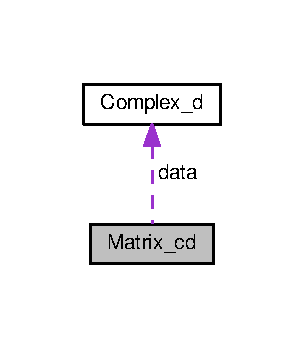
\includegraphics[width=146pt]{structMatrix__cd__coll__graph}
\end{center}
\end{figure}
\subsection*{Public Attributes}
\begin{DoxyCompactItemize}
\item 
M\+\_\+data\+\_\+type \hyperlink{structMatrix__cd_a258625d86cd44986cb352e84b7d5509d}{data\+\_\+type}
\item 
unsigned int \hyperlink{structMatrix__cd_a327b0893124ef84c447dcb9d08d14403}{row}
\item 
unsigned int \hyperlink{structMatrix__cd_a4b92706967cff4acd04999c4fc2ba8d6}{column}
\item 
\hyperlink{structComplex__d}{Complex\+\_\+d} $\ast$ \hyperlink{structMatrix__cd_ad754acb46b524029b61d1894c65aeace}{data}
\item 
M\+\_\+\+Property \hyperlink{structMatrix__cd_a346b2397657fec70767d3bbdd210a129}{prop}
\end{DoxyCompactItemize}


\subsection{Detailed Description}
complex double matrix type 

\subsection{Member Data Documentation}
\index{Matrix\+\_\+cd@{Matrix\+\_\+cd}!column@{column}}
\index{column@{column}!Matrix\+\_\+cd@{Matrix\+\_\+cd}}
\subsubsection[{\texorpdfstring{column}{column}}]{\setlength{\rightskip}{0pt plus 5cm}unsigned int Matrix\+\_\+cd\+::column}\hypertarget{structMatrix__cd_a4b92706967cff4acd04999c4fc2ba8d6}{}\label{structMatrix__cd_a4b92706967cff4acd04999c4fc2ba8d6}
number of columns of the matrix \index{Matrix\+\_\+cd@{Matrix\+\_\+cd}!data@{data}}
\index{data@{data}!Matrix\+\_\+cd@{Matrix\+\_\+cd}}
\subsubsection[{\texorpdfstring{data}{data}}]{\setlength{\rightskip}{0pt plus 5cm}{\bf Complex\+\_\+d}$\ast$ Matrix\+\_\+cd\+::data}\hypertarget{structMatrix__cd_ad754acb46b524029b61d1894c65aeace}{}\label{structMatrix__cd_ad754acb46b524029b61d1894c65aeace}
array containing the data \index{Matrix\+\_\+cd@{Matrix\+\_\+cd}!data\+\_\+type@{data\+\_\+type}}
\index{data\+\_\+type@{data\+\_\+type}!Matrix\+\_\+cd@{Matrix\+\_\+cd}}
\subsubsection[{\texorpdfstring{data\+\_\+type}{data_type}}]{\setlength{\rightskip}{0pt plus 5cm}M\+\_\+data\+\_\+type Matrix\+\_\+cd\+::data\+\_\+type}\hypertarget{structMatrix__cd_a258625d86cd44986cb352e84b7d5509d}{}\label{structMatrix__cd_a258625d86cd44986cb352e84b7d5509d}
type of data stored in the matrix -\/ used for verification \index{Matrix\+\_\+cd@{Matrix\+\_\+cd}!prop@{prop}}
\index{prop@{prop}!Matrix\+\_\+cd@{Matrix\+\_\+cd}}
\subsubsection[{\texorpdfstring{prop}{prop}}]{\setlength{\rightskip}{0pt plus 5cm}M\+\_\+\+Property Matrix\+\_\+cd\+::prop}\hypertarget{structMatrix__cd_a346b2397657fec70767d3bbdd210a129}{}\label{structMatrix__cd_a346b2397657fec70767d3bbdd210a129}
property of the matrix (for optimizations) \index{Matrix\+\_\+cd@{Matrix\+\_\+cd}!row@{row}}
\index{row@{row}!Matrix\+\_\+cd@{Matrix\+\_\+cd}}
\subsubsection[{\texorpdfstring{row}{row}}]{\setlength{\rightskip}{0pt plus 5cm}unsigned int Matrix\+\_\+cd\+::row}\hypertarget{structMatrix__cd_a327b0893124ef84c447dcb9d08d14403}{}\label{structMatrix__cd_a327b0893124ef84c447dcb9d08d14403}
number of rows of the matrix 

The documentation for this struct was generated from the following file\+:\begin{DoxyCompactItemize}
\item 
include/matrix\+\_\+type.\+h\end{DoxyCompactItemize}

\hypertarget{structMatrix__cf}{}\section{Matrix\+\_\+cf Struct Reference}
\label{structMatrix__cf}\index{Matrix\+\_\+cf@{Matrix\+\_\+cf}}


complex float matrix type  




{\ttfamily \#include $<$matrix\+\_\+type.\+h$>$}



Collaboration diagram for Matrix\+\_\+cf\+:\nopagebreak
\begin{figure}[H]
\begin{center}
\leavevmode
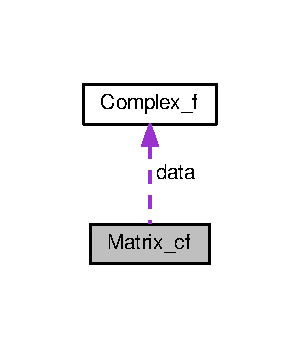
\includegraphics[width=144pt]{structMatrix__cf__coll__graph}
\end{center}
\end{figure}
\subsection*{Public Attributes}
\begin{DoxyCompactItemize}
\item 
M\+\_\+data\+\_\+type \hyperlink{structMatrix__cf_a93b82c3bbbc41c942eaa7891944a1015}{data\+\_\+type}
\item 
unsigned int \hyperlink{structMatrix__cf_a78fd97baf2f96f5277a90752322fd5a0}{row}
\item 
unsigned int \hyperlink{structMatrix__cf_ac0522815facf90db76974c3db9645927}{column}
\item 
\hyperlink{structComplex__f}{Complex\+\_\+f} $\ast$ \hyperlink{structMatrix__cf_a987beffa87c0ed47d1c7b23159c8fd31}{data}
\item 
M\+\_\+\+Property \hyperlink{structMatrix__cf_ae5e94ddc0ac8bd8bebfed98f3da07484}{prop}
\end{DoxyCompactItemize}


\subsection{Detailed Description}
complex float matrix type 

\subsection{Member Data Documentation}
\index{Matrix\+\_\+cf@{Matrix\+\_\+cf}!column@{column}}
\index{column@{column}!Matrix\+\_\+cf@{Matrix\+\_\+cf}}
\subsubsection[{\texorpdfstring{column}{column}}]{\setlength{\rightskip}{0pt plus 5cm}unsigned int Matrix\+\_\+cf\+::column}\hypertarget{structMatrix__cf_ac0522815facf90db76974c3db9645927}{}\label{structMatrix__cf_ac0522815facf90db76974c3db9645927}
number of columns of the matrix \index{Matrix\+\_\+cf@{Matrix\+\_\+cf}!data@{data}}
\index{data@{data}!Matrix\+\_\+cf@{Matrix\+\_\+cf}}
\subsubsection[{\texorpdfstring{data}{data}}]{\setlength{\rightskip}{0pt plus 5cm}{\bf Complex\+\_\+f}$\ast$ Matrix\+\_\+cf\+::data}\hypertarget{structMatrix__cf_a987beffa87c0ed47d1c7b23159c8fd31}{}\label{structMatrix__cf_a987beffa87c0ed47d1c7b23159c8fd31}
array containing the data \index{Matrix\+\_\+cf@{Matrix\+\_\+cf}!data\+\_\+type@{data\+\_\+type}}
\index{data\+\_\+type@{data\+\_\+type}!Matrix\+\_\+cf@{Matrix\+\_\+cf}}
\subsubsection[{\texorpdfstring{data\+\_\+type}{data_type}}]{\setlength{\rightskip}{0pt plus 5cm}M\+\_\+data\+\_\+type Matrix\+\_\+cf\+::data\+\_\+type}\hypertarget{structMatrix__cf_a93b82c3bbbc41c942eaa7891944a1015}{}\label{structMatrix__cf_a93b82c3bbbc41c942eaa7891944a1015}
type of data stored in the matrix -\/ used for verification \index{Matrix\+\_\+cf@{Matrix\+\_\+cf}!prop@{prop}}
\index{prop@{prop}!Matrix\+\_\+cf@{Matrix\+\_\+cf}}
\subsubsection[{\texorpdfstring{prop}{prop}}]{\setlength{\rightskip}{0pt plus 5cm}M\+\_\+\+Property Matrix\+\_\+cf\+::prop}\hypertarget{structMatrix__cf_ae5e94ddc0ac8bd8bebfed98f3da07484}{}\label{structMatrix__cf_ae5e94ddc0ac8bd8bebfed98f3da07484}
property of the matrix (for optimizations) \index{Matrix\+\_\+cf@{Matrix\+\_\+cf}!row@{row}}
\index{row@{row}!Matrix\+\_\+cf@{Matrix\+\_\+cf}}
\subsubsection[{\texorpdfstring{row}{row}}]{\setlength{\rightskip}{0pt plus 5cm}unsigned int Matrix\+\_\+cf\+::row}\hypertarget{structMatrix__cf_a78fd97baf2f96f5277a90752322fd5a0}{}\label{structMatrix__cf_a78fd97baf2f96f5277a90752322fd5a0}
number of rows of the matrix 

The documentation for this struct was generated from the following file\+:\begin{DoxyCompactItemize}
\item 
include/matrix\+\_\+type.\+h\end{DoxyCompactItemize}

\hypertarget{structMatrix__d}{}\section{Matrix\+\_\+d Struct Reference}
\label{structMatrix__d}\index{Matrix\+\_\+d@{Matrix\+\_\+d}}


double precision matrix type  




{\ttfamily \#include $<$matrix\+\_\+type.\+h$>$}

\subsection*{Public Attributes}
\begin{DoxyCompactItemize}
\item 
M\+\_\+data\+\_\+type \hyperlink{structMatrix__d_abd54be0a1d23b49811055d9c06690c5d}{data\+\_\+type}
\item 
unsigned int \hyperlink{structMatrix__d_ad4e549017d2d1c5dd83e76788de8a89d}{row}
\item 
unsigned int \hyperlink{structMatrix__d_afa4d9db2998b2fb84aa14db7ba8ae54f}{column}
\item 
double $\ast$ \hyperlink{structMatrix__d_a6a9f862ced230c4b29277846ed436c90}{data}
\item 
M\+\_\+\+Property \hyperlink{structMatrix__d_af7a8caafdd655171e1c6a9b1f532aa9a}{prop}
\end{DoxyCompactItemize}


\subsection{Detailed Description}
double precision matrix type 

\subsection{Member Data Documentation}
\index{Matrix\+\_\+d@{Matrix\+\_\+d}!column@{column}}
\index{column@{column}!Matrix\+\_\+d@{Matrix\+\_\+d}}
\subsubsection[{\texorpdfstring{column}{column}}]{\setlength{\rightskip}{0pt plus 5cm}unsigned int Matrix\+\_\+d\+::column}\hypertarget{structMatrix__d_afa4d9db2998b2fb84aa14db7ba8ae54f}{}\label{structMatrix__d_afa4d9db2998b2fb84aa14db7ba8ae54f}
number of columns of the matrix \index{Matrix\+\_\+d@{Matrix\+\_\+d}!data@{data}}
\index{data@{data}!Matrix\+\_\+d@{Matrix\+\_\+d}}
\subsubsection[{\texorpdfstring{data}{data}}]{\setlength{\rightskip}{0pt plus 5cm}double$\ast$ Matrix\+\_\+d\+::data}\hypertarget{structMatrix__d_a6a9f862ced230c4b29277846ed436c90}{}\label{structMatrix__d_a6a9f862ced230c4b29277846ed436c90}
array containing the data \index{Matrix\+\_\+d@{Matrix\+\_\+d}!data\+\_\+type@{data\+\_\+type}}
\index{data\+\_\+type@{data\+\_\+type}!Matrix\+\_\+d@{Matrix\+\_\+d}}
\subsubsection[{\texorpdfstring{data\+\_\+type}{data_type}}]{\setlength{\rightskip}{0pt plus 5cm}M\+\_\+data\+\_\+type Matrix\+\_\+d\+::data\+\_\+type}\hypertarget{structMatrix__d_abd54be0a1d23b49811055d9c06690c5d}{}\label{structMatrix__d_abd54be0a1d23b49811055d9c06690c5d}
type of data stored in the matrix -\/ used for verification \index{Matrix\+\_\+d@{Matrix\+\_\+d}!prop@{prop}}
\index{prop@{prop}!Matrix\+\_\+d@{Matrix\+\_\+d}}
\subsubsection[{\texorpdfstring{prop}{prop}}]{\setlength{\rightskip}{0pt plus 5cm}M\+\_\+\+Property Matrix\+\_\+d\+::prop}\hypertarget{structMatrix__d_af7a8caafdd655171e1c6a9b1f532aa9a}{}\label{structMatrix__d_af7a8caafdd655171e1c6a9b1f532aa9a}
property of the matrix (for optimizations) \index{Matrix\+\_\+d@{Matrix\+\_\+d}!row@{row}}
\index{row@{row}!Matrix\+\_\+d@{Matrix\+\_\+d}}
\subsubsection[{\texorpdfstring{row}{row}}]{\setlength{\rightskip}{0pt plus 5cm}unsigned int Matrix\+\_\+d\+::row}\hypertarget{structMatrix__d_ad4e549017d2d1c5dd83e76788de8a89d}{}\label{structMatrix__d_ad4e549017d2d1c5dd83e76788de8a89d}
number of rows of the matrix 

The documentation for this struct was generated from the following file\+:\begin{DoxyCompactItemize}
\item 
include/matrix\+\_\+type.\+h\end{DoxyCompactItemize}

\hypertarget{structMatrix__f}{}\section{Matrix\+\_\+f Struct Reference}
\label{structMatrix__f}\index{Matrix\+\_\+f@{Matrix\+\_\+f}}


floating point matrix type  




{\ttfamily \#include $<$matrix\+\_\+type.\+h$>$}

\subsection*{Public Attributes}
\begin{DoxyCompactItemize}
\item 
M\+\_\+data\+\_\+type \hyperlink{structMatrix__f_a208178d3dfeaa5adab42b96aff8c97d5}{data\+\_\+type}
\item 
unsigned int \hyperlink{structMatrix__f_a1105833a934acf7f2a07b154c1733acf}{row}
\item 
unsigned int \hyperlink{structMatrix__f_a2dff146309a2461f46463286f2b99ffc}{column}
\item 
float $\ast$ \hyperlink{structMatrix__f_aad17369cd1b7acebc55379d862e821c2}{data}
\item 
M\+\_\+\+Property \hyperlink{structMatrix__f_a0f8b87b8012ab2ffa92fbe55b1009d71}{prop}
\end{DoxyCompactItemize}


\subsection{Detailed Description}
floating point matrix type 

\subsection{Member Data Documentation}
\index{Matrix\+\_\+f@{Matrix\+\_\+f}!column@{column}}
\index{column@{column}!Matrix\+\_\+f@{Matrix\+\_\+f}}
\subsubsection[{\texorpdfstring{column}{column}}]{\setlength{\rightskip}{0pt plus 5cm}unsigned int Matrix\+\_\+f\+::column}\hypertarget{structMatrix__f_a2dff146309a2461f46463286f2b99ffc}{}\label{structMatrix__f_a2dff146309a2461f46463286f2b99ffc}
number of columns of the matrix \index{Matrix\+\_\+f@{Matrix\+\_\+f}!data@{data}}
\index{data@{data}!Matrix\+\_\+f@{Matrix\+\_\+f}}
\subsubsection[{\texorpdfstring{data}{data}}]{\setlength{\rightskip}{0pt plus 5cm}float$\ast$ Matrix\+\_\+f\+::data}\hypertarget{structMatrix__f_aad17369cd1b7acebc55379d862e821c2}{}\label{structMatrix__f_aad17369cd1b7acebc55379d862e821c2}
array containing the data \index{Matrix\+\_\+f@{Matrix\+\_\+f}!data\+\_\+type@{data\+\_\+type}}
\index{data\+\_\+type@{data\+\_\+type}!Matrix\+\_\+f@{Matrix\+\_\+f}}
\subsubsection[{\texorpdfstring{data\+\_\+type}{data_type}}]{\setlength{\rightskip}{0pt plus 5cm}M\+\_\+data\+\_\+type Matrix\+\_\+f\+::data\+\_\+type}\hypertarget{structMatrix__f_a208178d3dfeaa5adab42b96aff8c97d5}{}\label{structMatrix__f_a208178d3dfeaa5adab42b96aff8c97d5}
type of data stored in the matrix -\/ used for verification \index{Matrix\+\_\+f@{Matrix\+\_\+f}!prop@{prop}}
\index{prop@{prop}!Matrix\+\_\+f@{Matrix\+\_\+f}}
\subsubsection[{\texorpdfstring{prop}{prop}}]{\setlength{\rightskip}{0pt plus 5cm}M\+\_\+\+Property Matrix\+\_\+f\+::prop}\hypertarget{structMatrix__f_a0f8b87b8012ab2ffa92fbe55b1009d71}{}\label{structMatrix__f_a0f8b87b8012ab2ffa92fbe55b1009d71}
property of the matrix (for optimizations) \index{Matrix\+\_\+f@{Matrix\+\_\+f}!row@{row}}
\index{row@{row}!Matrix\+\_\+f@{Matrix\+\_\+f}}
\subsubsection[{\texorpdfstring{row}{row}}]{\setlength{\rightskip}{0pt plus 5cm}unsigned int Matrix\+\_\+f\+::row}\hypertarget{structMatrix__f_a1105833a934acf7f2a07b154c1733acf}{}\label{structMatrix__f_a1105833a934acf7f2a07b154c1733acf}
number of rows of the matrix 

The documentation for this struct was generated from the following file\+:\begin{DoxyCompactItemize}
\item 
include/matrix\+\_\+type.\+h\end{DoxyCompactItemize}

\hypertarget{structMatrix__i}{}\section{Matrix\+\_\+i Struct Reference}
\label{structMatrix__i}\index{Matrix\+\_\+i@{Matrix\+\_\+i}}


integer matrix type  




{\ttfamily \#include $<$matrix\+\_\+type.\+h$>$}

\subsection*{Public Attributes}
\begin{DoxyCompactItemize}
\item 
M\+\_\+data\+\_\+type \hyperlink{structMatrix__i_a099b6cf6ea02b60b50fafa042e48c063}{data\+\_\+type}
\item 
unsigned int \hyperlink{structMatrix__i_a9fc27d070aaebd0e2d7198a62f7b25d6}{row}
\item 
unsigned int \hyperlink{structMatrix__i_ae8f97821a7cb3ea2c6b4daa452f65c02}{column}
\item 
int $\ast$ \hyperlink{structMatrix__i_a0fe0365ed38d16792c645305c5662f53}{data}
\item 
M\+\_\+\+Property \hyperlink{structMatrix__i_a8b30ae67887da20fe1d7fdd51ebc3ecb}{prop}
\end{DoxyCompactItemize}


\subsection{Detailed Description}
integer matrix type 

\subsection{Member Data Documentation}
\index{Matrix\+\_\+i@{Matrix\+\_\+i}!column@{column}}
\index{column@{column}!Matrix\+\_\+i@{Matrix\+\_\+i}}
\subsubsection[{\texorpdfstring{column}{column}}]{\setlength{\rightskip}{0pt plus 5cm}unsigned int Matrix\+\_\+i\+::column}\hypertarget{structMatrix__i_ae8f97821a7cb3ea2c6b4daa452f65c02}{}\label{structMatrix__i_ae8f97821a7cb3ea2c6b4daa452f65c02}
number of columns of the matrix \index{Matrix\+\_\+i@{Matrix\+\_\+i}!data@{data}}
\index{data@{data}!Matrix\+\_\+i@{Matrix\+\_\+i}}
\subsubsection[{\texorpdfstring{data}{data}}]{\setlength{\rightskip}{0pt plus 5cm}int$\ast$ Matrix\+\_\+i\+::data}\hypertarget{structMatrix__i_a0fe0365ed38d16792c645305c5662f53}{}\label{structMatrix__i_a0fe0365ed38d16792c645305c5662f53}
array containing the data \index{Matrix\+\_\+i@{Matrix\+\_\+i}!data\+\_\+type@{data\+\_\+type}}
\index{data\+\_\+type@{data\+\_\+type}!Matrix\+\_\+i@{Matrix\+\_\+i}}
\subsubsection[{\texorpdfstring{data\+\_\+type}{data_type}}]{\setlength{\rightskip}{0pt plus 5cm}M\+\_\+data\+\_\+type Matrix\+\_\+i\+::data\+\_\+type}\hypertarget{structMatrix__i_a099b6cf6ea02b60b50fafa042e48c063}{}\label{structMatrix__i_a099b6cf6ea02b60b50fafa042e48c063}
type of data stored in the matrix -\/ used for verification \index{Matrix\+\_\+i@{Matrix\+\_\+i}!prop@{prop}}
\index{prop@{prop}!Matrix\+\_\+i@{Matrix\+\_\+i}}
\subsubsection[{\texorpdfstring{prop}{prop}}]{\setlength{\rightskip}{0pt plus 5cm}M\+\_\+\+Property Matrix\+\_\+i\+::prop}\hypertarget{structMatrix__i_a8b30ae67887da20fe1d7fdd51ebc3ecb}{}\label{structMatrix__i_a8b30ae67887da20fe1d7fdd51ebc3ecb}
property of the matrix (for optimizations) \index{Matrix\+\_\+i@{Matrix\+\_\+i}!row@{row}}
\index{row@{row}!Matrix\+\_\+i@{Matrix\+\_\+i}}
\subsubsection[{\texorpdfstring{row}{row}}]{\setlength{\rightskip}{0pt plus 5cm}unsigned int Matrix\+\_\+i\+::row}\hypertarget{structMatrix__i_a9fc27d070aaebd0e2d7198a62f7b25d6}{}\label{structMatrix__i_a9fc27d070aaebd0e2d7198a62f7b25d6}
number of rows of the matrix 

The documentation for this struct was generated from the following file\+:\begin{DoxyCompactItemize}
\item 
matrix\+\_\+type.\+h\end{DoxyCompactItemize}

\chapter{File Documentation}
\hypertarget{complex__d_8c}{}\section{source/complex\+\_\+d.c File Reference}
\label{complex__d_8c}\index{source/complex\+\_\+d.\+c@{source/complex\+\_\+d.\+c}}
{\ttfamily \#include $<$stdio.\+h$>$}\\*
{\ttfamily \#include $<$stdlib.\+h$>$}\\*
{\ttfamily \#include $<$math.\+h$>$}\\*
{\ttfamily \#include \char`\"{}../include/complex\+\_\+d.\+h\char`\"{}}\\*
Include dependency graph for complex\+\_\+d.\+c\+:
\nopagebreak
\begin{figure}[H]
\begin{center}
\leavevmode
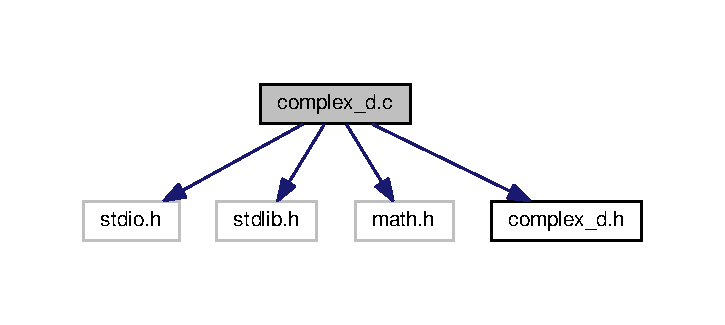
\includegraphics[width=350pt]{complex__d_8c__incl}
\end{center}
\end{figure}
\subsection*{Functions}
\begin{DoxyCompactItemize}
\item 
int \hyperlink{complex__d_8c_a410d1fb6ecb863dced8eae062b6819ae}{equals\+\_\+d} (double a, double b, double precis)
\begin{DoxyCompactList}\small\item\em test the equality of two doubles relatively to a precision \end{DoxyCompactList}\item 
int \hyperlink{complex__d_8c_adcf616a76b82a6814443352eda851dd9}{is\+Null\+\_\+d} (\hyperlink{structComplex__d}{Complex\+\_\+d} a)
\begin{DoxyCompactList}\small\item\em test if a complex is N\+U\+LL relatively to a precision \end{DoxyCompactList}\item 
\hyperlink{structComplex__d}{Complex\+\_\+d} \hyperlink{complex__d_8c_a6ab5931e3760650c97f8cd91eae5ec98}{conjugateD} (\hyperlink{structComplex__d}{Complex\+\_\+d} c)
\begin{DoxyCompactList}\small\item\em conjugateD computes the conjugate of a complex \end{DoxyCompactList}\item 
\hyperlink{structComplex__d}{Complex\+\_\+d} \hyperlink{complex__d_8c_a6033654f35e0e520cd852b9d2c0c00d3}{addD} (\hyperlink{structComplex__d}{Complex\+\_\+d} a, \hyperlink{structComplex__d}{Complex\+\_\+d} b)
\begin{DoxyCompactList}\small\item\em addD add two complexes \end{DoxyCompactList}\item 
\hyperlink{structComplex__d}{Complex\+\_\+d} \hyperlink{complex__d_8c_a5db14373c0c0eb91f28d518faa9c24cc}{subD} (\hyperlink{structComplex__d}{Complex\+\_\+d} a, \hyperlink{structComplex__d}{Complex\+\_\+d} b)
\begin{DoxyCompactList}\small\item\em subD substract two complexes (a-\/b) \end{DoxyCompactList}\item 
\hyperlink{structComplex__d}{Complex\+\_\+d} \hyperlink{complex__d_8c_a52d29ba6af386de1f57288864dceb97b}{scaleD} (\hyperlink{structComplex__d}{Complex\+\_\+d} a, double c)
\begin{DoxyCompactList}\small\item\em scaleD multiply a complex by a constant \end{DoxyCompactList}\item 
\hyperlink{structComplex__d}{Complex\+\_\+d} \hyperlink{complex__d_8c_a570534360c43b7bfd09dff1c1bfcc15a}{multiplyD} (\hyperlink{structComplex__d}{Complex\+\_\+d} a, \hyperlink{structComplex__d}{Complex\+\_\+d} b)
\begin{DoxyCompactList}\small\item\em multiplyD multiply two complexes \end{DoxyCompactList}\item 
\hyperlink{structComplex__d}{Complex\+\_\+d} \hyperlink{complex__d_8c_a8c9dc9ae5499b8770456306768908d67}{divD} (\hyperlink{structComplex__d}{Complex\+\_\+d} a, \hyperlink{structComplex__d}{Complex\+\_\+d} b)
\begin{DoxyCompactList}\small\item\em divD divide two complexes (a/b) \end{DoxyCompactList}\item 
\hyperlink{structComplex__d}{Complex\+\_\+d} \hyperlink{complex__d_8c_a45be7d0c6d3bce5608312e7968342b95}{invD} (\hyperlink{structComplex__d}{Complex\+\_\+d} a)
\begin{DoxyCompactList}\small\item\em invD compute the inverse of a complex \end{DoxyCompactList}\item 
\hyperlink{structComplex__d}{Complex\+\_\+d} \hyperlink{complex__d_8c_a54566d94a5cf745c4e6d9e35df555983}{multiply\+By\+ConjD} (\hyperlink{structComplex__d}{Complex\+\_\+d} a)
\begin{DoxyCompactList}\small\item\em multiply\+By\+ConjD multiply a complex by it\textquotesingle{}s conjugate \end{DoxyCompactList}\item 
double \hyperlink{complex__d_8c_abec8399c803b374893649400e77f12e3}{gainD} (\hyperlink{structComplex__d}{Complex\+\_\+d} a)
\begin{DoxyCompactList}\small\item\em gainD compute the gain of a complex \end{DoxyCompactList}\item 
\hyperlink{structComplex__d}{Complex\+\_\+d} \hyperlink{complex__d_8c_ac5473583db7db01b4bdc6add24d50b20}{create\+Nul\+ComplexD} (void)
\begin{DoxyCompactList}\small\item\em create\+Nul\+ComplexD create a complex 0 + 0$\ast$i \end{DoxyCompactList}\item 
\hyperlink{structComplex__d}{Complex\+\_\+d} \hyperlink{complex__d_8c_ad578ab4068a3eaec4069176a740711b3}{create\+Unitary\+ComplexD} (void)
\begin{DoxyCompactList}\small\item\em create\+Unitary\+ComplexD create a complex 1 + 1$\ast$i \end{DoxyCompactList}\item 
\hyperlink{structComplex__d}{Complex\+\_\+d} \hyperlink{complex__d_8c_ad7fb9b177d271669a68cabbb1c963732}{create\+Random\+ComplexD} (void)
\begin{DoxyCompactList}\small\item\em create\+Random\+ComplexD create a random complex \end{DoxyCompactList}\item 
\hyperlink{structComplex__d}{Complex\+\_\+d} \hyperlink{complex__d_8c_ac18d884c91c84217cab8ed87b0512db2}{create\+ComplexD} (double re, double im)
\begin{DoxyCompactList}\small\item\em creat\+ComplexD create a complex by receiving real and imaginary part \end{DoxyCompactList}\item 
void \hyperlink{complex__d_8c_acb49a177e60ea9d661664e15d661d30d}{print\+ComplexD} (\hyperlink{structComplex__d}{Complex\+\_\+d} a)\hypertarget{complex__d_8c_acb49a177e60ea9d661664e15d661d30d}{}\label{complex__d_8c_acb49a177e60ea9d661664e15d661d30d}

\begin{DoxyCompactList}\small\item\em printf a complex \end{DoxyCompactList}\end{DoxyCompactItemize}


\subsection{Detailed Description}
to handle basic complexes functions \begin{DoxyAuthor}{Author}
Nicolas Sourbier 
\end{DoxyAuthor}
\begin{DoxyDate}{Date}
10/09/2018 
\end{DoxyDate}


\subsection{Function Documentation}
\index{complex\+\_\+d.\+c@{complex\+\_\+d.\+c}!addD@{addD}}
\index{addD@{addD}!complex\+\_\+d.\+c@{complex\+\_\+d.\+c}}
\subsubsection[{\texorpdfstring{add\+D(\+Complex\+\_\+d a, Complex\+\_\+d b)}{addD(Complex_d a, Complex_d b)}}]{\setlength{\rightskip}{0pt plus 5cm}{\bf Complex\+\_\+d} addD (
\begin{DoxyParamCaption}
\item[{{\bf Complex\+\_\+d}}]{a, }
\item[{{\bf Complex\+\_\+d}}]{b}
\end{DoxyParamCaption}
)}\hypertarget{complex__d_8c_a6033654f35e0e520cd852b9d2c0c00d3}{}\label{complex__d_8c_a6033654f35e0e520cd852b9d2c0c00d3}


addD add two complexes 


\begin{DoxyParams}{Parameters}
{\em a} & the first operand \\
\hline
{\em b} & the complex to add to the first one \\
\hline
\end{DoxyParams}
\begin{DoxyReturn}{Returns}
the sum of the two complexes 
\end{DoxyReturn}
\index{complex\+\_\+d.\+c@{complex\+\_\+d.\+c}!conjugateD@{conjugateD}}
\index{conjugateD@{conjugateD}!complex\+\_\+d.\+c@{complex\+\_\+d.\+c}}
\subsubsection[{\texorpdfstring{conjugate\+D(\+Complex\+\_\+d c)}{conjugateD(Complex_d c)}}]{\setlength{\rightskip}{0pt plus 5cm}{\bf Complex\+\_\+d} conjugateD (
\begin{DoxyParamCaption}
\item[{{\bf Complex\+\_\+d}}]{c}
\end{DoxyParamCaption}
)}\hypertarget{complex__d_8c_a6ab5931e3760650c97f8cd91eae5ec98}{}\label{complex__d_8c_a6ab5931e3760650c97f8cd91eae5ec98}


conjugateD computes the conjugate of a complex 


\begin{DoxyParams}{Parameters}
{\em c} & the complex we want to know the conjugate \\
\hline
\end{DoxyParams}
\begin{DoxyReturn}{Returns}
a new complex containing the conjugate of the one given in param 
\end{DoxyReturn}
\index{complex\+\_\+d.\+c@{complex\+\_\+d.\+c}!create\+ComplexD@{create\+ComplexD}}
\index{create\+ComplexD@{create\+ComplexD}!complex\+\_\+d.\+c@{complex\+\_\+d.\+c}}
\subsubsection[{\texorpdfstring{create\+Complex\+D(double re, double im)}{createComplexD(double re, double im)}}]{\setlength{\rightskip}{0pt plus 5cm}{\bf Complex\+\_\+d} create\+ComplexD (
\begin{DoxyParamCaption}
\item[{double}]{re, }
\item[{double}]{im}
\end{DoxyParamCaption}
)}\hypertarget{complex__d_8c_ac18d884c91c84217cab8ed87b0512db2}{}\label{complex__d_8c_ac18d884c91c84217cab8ed87b0512db2}


creat\+ComplexD create a complex by receiving real and imaginary part 

\begin{DoxyReturn}{Returns}
a random complex 
\end{DoxyReturn}
\index{complex\+\_\+d.\+c@{complex\+\_\+d.\+c}!create\+Nul\+ComplexD@{create\+Nul\+ComplexD}}
\index{create\+Nul\+ComplexD@{create\+Nul\+ComplexD}!complex\+\_\+d.\+c@{complex\+\_\+d.\+c}}
\subsubsection[{\texorpdfstring{create\+Nul\+Complex\+D(void)}{createNulComplexD(void)}}]{\setlength{\rightskip}{0pt plus 5cm}{\bf Complex\+\_\+d} create\+Nul\+ComplexD (
\begin{DoxyParamCaption}
\item[{void}]{}
\end{DoxyParamCaption}
)}\hypertarget{complex__d_8c_ac5473583db7db01b4bdc6add24d50b20}{}\label{complex__d_8c_ac5473583db7db01b4bdc6add24d50b20}


create\+Nul\+ComplexD create a complex 0 + 0$\ast$i 

\begin{DoxyReturn}{Returns}
a nul complex 
\end{DoxyReturn}
\index{complex\+\_\+d.\+c@{complex\+\_\+d.\+c}!create\+Random\+ComplexD@{create\+Random\+ComplexD}}
\index{create\+Random\+ComplexD@{create\+Random\+ComplexD}!complex\+\_\+d.\+c@{complex\+\_\+d.\+c}}
\subsubsection[{\texorpdfstring{create\+Random\+Complex\+D(void)}{createRandomComplexD(void)}}]{\setlength{\rightskip}{0pt plus 5cm}{\bf Complex\+\_\+d} create\+Random\+ComplexD (
\begin{DoxyParamCaption}
\item[{void}]{}
\end{DoxyParamCaption}
)}\hypertarget{complex__d_8c_ad7fb9b177d271669a68cabbb1c963732}{}\label{complex__d_8c_ad7fb9b177d271669a68cabbb1c963732}


create\+Random\+ComplexD create a random complex 

\begin{DoxyReturn}{Returns}
a random complex 
\end{DoxyReturn}
\index{complex\+\_\+d.\+c@{complex\+\_\+d.\+c}!create\+Unitary\+ComplexD@{create\+Unitary\+ComplexD}}
\index{create\+Unitary\+ComplexD@{create\+Unitary\+ComplexD}!complex\+\_\+d.\+c@{complex\+\_\+d.\+c}}
\subsubsection[{\texorpdfstring{create\+Unitary\+Complex\+D(void)}{createUnitaryComplexD(void)}}]{\setlength{\rightskip}{0pt plus 5cm}{\bf Complex\+\_\+d} create\+Unitary\+ComplexD (
\begin{DoxyParamCaption}
\item[{void}]{}
\end{DoxyParamCaption}
)}\hypertarget{complex__d_8c_ad578ab4068a3eaec4069176a740711b3}{}\label{complex__d_8c_ad578ab4068a3eaec4069176a740711b3}


create\+Unitary\+ComplexD create a complex 1 + 1$\ast$i 

\begin{DoxyReturn}{Returns}
a complex with a real an imaginary part of 1 
\end{DoxyReturn}
\index{complex\+\_\+d.\+c@{complex\+\_\+d.\+c}!divD@{divD}}
\index{divD@{divD}!complex\+\_\+d.\+c@{complex\+\_\+d.\+c}}
\subsubsection[{\texorpdfstring{div\+D(\+Complex\+\_\+d a, Complex\+\_\+d b)}{divD(Complex_d a, Complex_d b)}}]{\setlength{\rightskip}{0pt plus 5cm}{\bf Complex\+\_\+d} divD (
\begin{DoxyParamCaption}
\item[{{\bf Complex\+\_\+d}}]{a, }
\item[{{\bf Complex\+\_\+d}}]{b}
\end{DoxyParamCaption}
)}\hypertarget{complex__d_8c_a8c9dc9ae5499b8770456306768908d67}{}\label{complex__d_8c_a8c9dc9ae5499b8770456306768908d67}


divD divide two complexes (a/b) 

\begin{DoxyReturn}{Returns}
the quotient of the two 
\end{DoxyReturn}
\index{complex\+\_\+d.\+c@{complex\+\_\+d.\+c}!equals\+\_\+d@{equals\+\_\+d}}
\index{equals\+\_\+d@{equals\+\_\+d}!complex\+\_\+d.\+c@{complex\+\_\+d.\+c}}
\subsubsection[{\texorpdfstring{equals\+\_\+d(double a, double b, double precis)}{equals_d(double a, double b, double precis)}}]{\setlength{\rightskip}{0pt plus 5cm}int equals\+\_\+d (
\begin{DoxyParamCaption}
\item[{double}]{a, }
\item[{double}]{b, }
\item[{double}]{precis}
\end{DoxyParamCaption}
)}\hypertarget{complex__d_8c_a410d1fb6ecb863dced8eae062b6819ae}{}\label{complex__d_8c_a410d1fb6ecb863dced8eae062b6819ae}


test the equality of two doubles relatively to a precision 


\begin{DoxyParams}{Parameters}
{\em a} & and \\
\hline
{\em b} & the doubles to compare. \\
\hline
{\em precis} & the precision of the comparison \\
\hline
\end{DoxyParams}
\begin{DoxyReturn}{Returns}
1 if equal, 0 otherwise 
\end{DoxyReturn}
\index{complex\+\_\+d.\+c@{complex\+\_\+d.\+c}!gainD@{gainD}}
\index{gainD@{gainD}!complex\+\_\+d.\+c@{complex\+\_\+d.\+c}}
\subsubsection[{\texorpdfstring{gain\+D(\+Complex\+\_\+d a)}{gainD(Complex_d a)}}]{\setlength{\rightskip}{0pt plus 5cm}double gainD (
\begin{DoxyParamCaption}
\item[{{\bf Complex\+\_\+d}}]{a}
\end{DoxyParamCaption}
)}\hypertarget{complex__d_8c_abec8399c803b374893649400e77f12e3}{}\label{complex__d_8c_abec8399c803b374893649400e77f12e3}


gainD compute the gain of a complex 


\begin{DoxyParams}{Parameters}
{\em a} & the complex we want to know the gain \\
\hline
\end{DoxyParams}
\begin{DoxyReturn}{Returns}
the gain of the complex 
\end{DoxyReturn}
\index{complex\+\_\+d.\+c@{complex\+\_\+d.\+c}!invD@{invD}}
\index{invD@{invD}!complex\+\_\+d.\+c@{complex\+\_\+d.\+c}}
\subsubsection[{\texorpdfstring{inv\+D(\+Complex\+\_\+d a)}{invD(Complex_d a)}}]{\setlength{\rightskip}{0pt plus 5cm}{\bf Complex\+\_\+d} invD (
\begin{DoxyParamCaption}
\item[{{\bf Complex\+\_\+d}}]{a}
\end{DoxyParamCaption}
)}\hypertarget{complex__d_8c_a45be7d0c6d3bce5608312e7968342b95}{}\label{complex__d_8c_a45be7d0c6d3bce5608312e7968342b95}


invD compute the inverse of a complex 


\begin{DoxyParams}{Parameters}
{\em a} & the complex to invert \\
\hline
\end{DoxyParams}
\begin{DoxyReturn}{Returns}
the inverted complex 
\end{DoxyReturn}
\index{complex\+\_\+d.\+c@{complex\+\_\+d.\+c}!is\+Null\+\_\+d@{is\+Null\+\_\+d}}
\index{is\+Null\+\_\+d@{is\+Null\+\_\+d}!complex\+\_\+d.\+c@{complex\+\_\+d.\+c}}
\subsubsection[{\texorpdfstring{is\+Null\+\_\+d(\+Complex\+\_\+d a)}{isNull_d(Complex_d a)}}]{\setlength{\rightskip}{0pt plus 5cm}int is\+Null\+\_\+d (
\begin{DoxyParamCaption}
\item[{{\bf Complex\+\_\+d}}]{a}
\end{DoxyParamCaption}
)}\hypertarget{complex__d_8c_adcf616a76b82a6814443352eda851dd9}{}\label{complex__d_8c_adcf616a76b82a6814443352eda851dd9}


test if a complex is N\+U\+LL relatively to a precision 


\begin{DoxyParams}{Parameters}
{\em a} & and b, the doubles to compare \\
\hline
\end{DoxyParams}
\begin{DoxyReturn}{Returns}
1 if equal, 0 otherwise 
\end{DoxyReturn}
\index{complex\+\_\+d.\+c@{complex\+\_\+d.\+c}!multiply\+By\+ConjD@{multiply\+By\+ConjD}}
\index{multiply\+By\+ConjD@{multiply\+By\+ConjD}!complex\+\_\+d.\+c@{complex\+\_\+d.\+c}}
\subsubsection[{\texorpdfstring{multiply\+By\+Conj\+D(\+Complex\+\_\+d a)}{multiplyByConjD(Complex_d a)}}]{\setlength{\rightskip}{0pt plus 5cm}{\bf Complex\+\_\+d} multiply\+By\+ConjD (
\begin{DoxyParamCaption}
\item[{{\bf Complex\+\_\+d}}]{a}
\end{DoxyParamCaption}
)}\hypertarget{complex__d_8c_a54566d94a5cf745c4e6d9e35df555983}{}\label{complex__d_8c_a54566d94a5cf745c4e6d9e35df555983}


multiply\+By\+ConjD multiply a complex by it\textquotesingle{}s conjugate 


\begin{DoxyParams}{Parameters}
{\em a} & the complex to multiply \\
\hline
\end{DoxyParams}
\begin{DoxyReturn}{Returns}
the product of the complex and it\textquotesingle{}s conjugate 
\end{DoxyReturn}
\index{complex\+\_\+d.\+c@{complex\+\_\+d.\+c}!multiplyD@{multiplyD}}
\index{multiplyD@{multiplyD}!complex\+\_\+d.\+c@{complex\+\_\+d.\+c}}
\subsubsection[{\texorpdfstring{multiply\+D(\+Complex\+\_\+d a, Complex\+\_\+d b)}{multiplyD(Complex_d a, Complex_d b)}}]{\setlength{\rightskip}{0pt plus 5cm}{\bf Complex\+\_\+d} multiplyD (
\begin{DoxyParamCaption}
\item[{{\bf Complex\+\_\+d}}]{a, }
\item[{{\bf Complex\+\_\+d}}]{b}
\end{DoxyParamCaption}
)}\hypertarget{complex__d_8c_a570534360c43b7bfd09dff1c1bfcc15a}{}\label{complex__d_8c_a570534360c43b7bfd09dff1c1bfcc15a}


multiplyD multiply two complexes 

\begin{DoxyReturn}{Returns}
the product of a and b 
\end{DoxyReturn}
\index{complex\+\_\+d.\+c@{complex\+\_\+d.\+c}!scaleD@{scaleD}}
\index{scaleD@{scaleD}!complex\+\_\+d.\+c@{complex\+\_\+d.\+c}}
\subsubsection[{\texorpdfstring{scale\+D(\+Complex\+\_\+d a, double c)}{scaleD(Complex_d a, double c)}}]{\setlength{\rightskip}{0pt plus 5cm}{\bf Complex\+\_\+d} scaleD (
\begin{DoxyParamCaption}
\item[{{\bf Complex\+\_\+d}}]{a, }
\item[{double}]{c}
\end{DoxyParamCaption}
)}\hypertarget{complex__d_8c_a52d29ba6af386de1f57288864dceb97b}{}\label{complex__d_8c_a52d29ba6af386de1f57288864dceb97b}


scaleD multiply a complex by a constant 

\begin{DoxyReturn}{Returns}
the product of a and c 
\end{DoxyReturn}
\index{complex\+\_\+d.\+c@{complex\+\_\+d.\+c}!subD@{subD}}
\index{subD@{subD}!complex\+\_\+d.\+c@{complex\+\_\+d.\+c}}
\subsubsection[{\texorpdfstring{sub\+D(\+Complex\+\_\+d a, Complex\+\_\+d b)}{subD(Complex_d a, Complex_d b)}}]{\setlength{\rightskip}{0pt plus 5cm}{\bf Complex\+\_\+d} subD (
\begin{DoxyParamCaption}
\item[{{\bf Complex\+\_\+d}}]{a, }
\item[{{\bf Complex\+\_\+d}}]{b}
\end{DoxyParamCaption}
)}\hypertarget{complex__d_8c_a5db14373c0c0eb91f28d518faa9c24cc}{}\label{complex__d_8c_a5db14373c0c0eb91f28d518faa9c24cc}


subD substract two complexes (a-\/b) 


\begin{DoxyParams}{Parameters}
{\em a} & the fist operand \\
\hline
{\em b} & the complex we want to substract \\
\hline
\end{DoxyParams}
\begin{DoxyReturn}{Returns}
the difference of the two 
\end{DoxyReturn}

\hypertarget{complex__f_8c}{}\section{source/complex\+\_\+f.c File Reference}
\label{complex__f_8c}\index{source/complex\+\_\+f.\+c@{source/complex\+\_\+f.\+c}}
{\ttfamily \#include \char`\"{}../include/complex\+\_\+f.\+h\char`\"{}}\\*
Include dependency graph for complex\+\_\+f.\+c\+:
\nopagebreak
\begin{figure}[H]
\begin{center}
\leavevmode
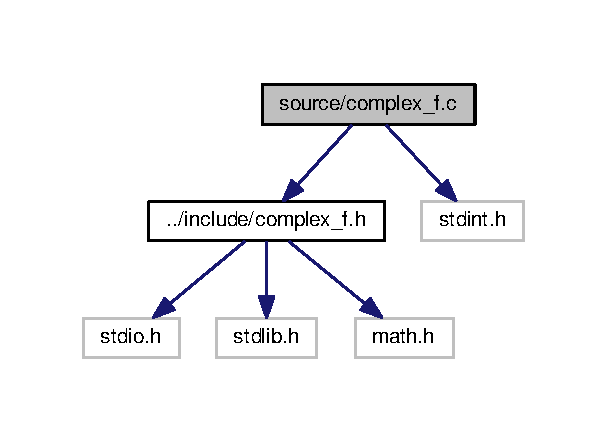
\includegraphics[width=258pt]{complex__f_8c__incl}
\end{center}
\end{figure}
\subsection*{Functions}
\begin{DoxyCompactItemize}
\item 
int \hyperlink{complex__f_8c_ae8d5115ead472e2bcbe978f146766274}{equals\+\_\+f} (float a, float b, float precis)
\begin{DoxyCompactList}\small\item\em test the equality of two floats relatively to a precision \end{DoxyCompactList}\item 
int \hyperlink{complex__f_8c_aa956ba70c67f43af6f2fb11a8f9d8248}{is\+Null\+\_\+f} (\hyperlink{structComplex__f}{Complex\+\_\+f} a)
\begin{DoxyCompactList}\small\item\em test if a complex is N\+U\+LL relatively to a precision \end{DoxyCompactList}\item 
\hyperlink{structComplex__f}{Complex\+\_\+f} \hyperlink{complex__f_8c_a3301aa4f26a5a781576428a8de2552b6}{conjugateF} (\hyperlink{structComplex__f}{Complex\+\_\+f} c)
\begin{DoxyCompactList}\small\item\em conjugateF computes the conjugate of a complex \end{DoxyCompactList}\item 
\hyperlink{structComplex__f}{Complex\+\_\+f} \hyperlink{complex__f_8c_ac4432be4524cb2d9a4272703ee26a285}{addF} (\hyperlink{structComplex__f}{Complex\+\_\+f} a, \hyperlink{structComplex__f}{Complex\+\_\+f} b)
\begin{DoxyCompactList}\small\item\em addF add two complexes \end{DoxyCompactList}\item 
\hyperlink{structComplex__f}{Complex\+\_\+f} \hyperlink{complex__f_8c_af097998e4898e6407ce54ed0da7280fb}{subF} (\hyperlink{structComplex__f}{Complex\+\_\+f} a, \hyperlink{structComplex__f}{Complex\+\_\+f} b)
\begin{DoxyCompactList}\small\item\em subF substract two complexes (a-\/b) \end{DoxyCompactList}\item 
\hyperlink{structComplex__f}{Complex\+\_\+f} \hyperlink{complex__f_8c_af7c74a571a7d93993389961b39ab125b}{scaleF} (\hyperlink{structComplex__f}{Complex\+\_\+f} a, float c)
\begin{DoxyCompactList}\small\item\em scaleF multiply a complex by a constant \end{DoxyCompactList}\item 
\hyperlink{structComplex__f}{Complex\+\_\+f} \hyperlink{complex__f_8c_ac068ed59ed029d889bc5328383c4ef83}{multiplyF} (\hyperlink{structComplex__f}{Complex\+\_\+f} a, \hyperlink{structComplex__f}{Complex\+\_\+f} b)
\begin{DoxyCompactList}\small\item\em multiplyF multiply two complexes \end{DoxyCompactList}\item 
\hyperlink{structComplex__f}{Complex\+\_\+f} \hyperlink{complex__f_8c_a9ff571018104b2884b663170e2150529}{divF} (\hyperlink{structComplex__f}{Complex\+\_\+f} a, \hyperlink{structComplex__f}{Complex\+\_\+f} b)
\begin{DoxyCompactList}\small\item\em divF divide two complexes (a/b) \end{DoxyCompactList}\item 
\hyperlink{structComplex__f}{Complex\+\_\+f} \hyperlink{complex__f_8c_a7364dda425aef124dda1f89f8b90d51d}{invF} (\hyperlink{structComplex__f}{Complex\+\_\+f} a)
\begin{DoxyCompactList}\small\item\em invF compute the inverse of a complex \end{DoxyCompactList}\item 
\hyperlink{structComplex__f}{Complex\+\_\+f} \hyperlink{complex__f_8c_ac14f07fc64e02dfe2bf7fc49ea281a10}{multiply\+By\+ConjF} (\hyperlink{structComplex__f}{Complex\+\_\+f} a)
\begin{DoxyCompactList}\small\item\em multiply\+By\+ConjF multiply a complex by it\textquotesingle{}s conjugate \end{DoxyCompactList}\item 
float \hyperlink{complex__f_8c_a9bfe41c65910e65f180972038e46881c}{gainF} (\hyperlink{structComplex__f}{Complex\+\_\+f} a)
\begin{DoxyCompactList}\small\item\em gainF compute the gain of a complex \end{DoxyCompactList}\item 
\hyperlink{structComplex__f}{Complex\+\_\+f} \hyperlink{complex__f_8c_a9ae6e848a8ae74ba0a132b4bdeee49fa}{create\+Nul\+ComplexF} (void)
\begin{DoxyCompactList}\small\item\em create\+Nul\+ComplexF create a complex 0 + 0$\ast$i \end{DoxyCompactList}\item 
\hyperlink{structComplex__f}{Complex\+\_\+f} \hyperlink{complex__f_8c_a4d3670cdd83a0e55d28c390476804f63}{create\+Unitary\+ComplexF} (void)
\begin{DoxyCompactList}\small\item\em create\+Unitary\+ComplexF create a complex 1 + 1$\ast$i \end{DoxyCompactList}\item 
\hyperlink{structComplex__f}{Complex\+\_\+f} \hyperlink{complex__f_8c_a04fb1df1f2eb4b9a2dde1e40ac565d4a}{create\+Random\+ComplexF} (void)
\begin{DoxyCompactList}\small\item\em create\+Random\+ComplexF create a random complex \end{DoxyCompactList}\item 
\hyperlink{structComplex__f}{Complex\+\_\+f} \hyperlink{complex__f_8c_a5c7b3c84b75536ccacada45b40f045b0}{create\+ComplexF} (float re, float im)
\begin{DoxyCompactList}\small\item\em creat\+ComplexF create a complex by receiving real and imaginary part \end{DoxyCompactList}\item 
void \hyperlink{complex__f_8c_aa9aa28014d061f3819017e9fa7befe8a}{print\+ComplexF} (\hyperlink{structComplex__f}{Complex\+\_\+f} a)\hypertarget{complex__f_8c_aa9aa28014d061f3819017e9fa7befe8a}{}\label{complex__f_8c_aa9aa28014d061f3819017e9fa7befe8a}

\begin{DoxyCompactList}\small\item\em printf a complex \end{DoxyCompactList}\end{DoxyCompactItemize}


\subsection{Detailed Description}
to handle basic complexes functions \begin{DoxyAuthor}{Author}
Nicolas Sourbier 
\end{DoxyAuthor}
\begin{DoxyDate}{Date}
10/09/2018 
\end{DoxyDate}


\subsection{Function Documentation}
\index{complex\+\_\+f.\+c@{complex\+\_\+f.\+c}!addF@{addF}}
\index{addF@{addF}!complex\+\_\+f.\+c@{complex\+\_\+f.\+c}}
\subsubsection[{\texorpdfstring{add\+F(\+Complex\+\_\+f a, Complex\+\_\+f b)}{addF(Complex_f a, Complex_f b)}}]{\setlength{\rightskip}{0pt plus 5cm}{\bf Complex\+\_\+f} addF (
\begin{DoxyParamCaption}
\item[{{\bf Complex\+\_\+f}}]{a, }
\item[{{\bf Complex\+\_\+f}}]{b}
\end{DoxyParamCaption}
)}\hypertarget{complex__f_8c_ac4432be4524cb2d9a4272703ee26a285}{}\label{complex__f_8c_ac4432be4524cb2d9a4272703ee26a285}


addF add two complexes 


\begin{DoxyParams}{Parameters}
{\em a} & the first operand \\
\hline
{\em b} & the complex to add to the first one \\
\hline
\end{DoxyParams}
\begin{DoxyReturn}{Returns}
the sum of the two complexes 
\end{DoxyReturn}
\index{complex\+\_\+f.\+c@{complex\+\_\+f.\+c}!conjugateF@{conjugateF}}
\index{conjugateF@{conjugateF}!complex\+\_\+f.\+c@{complex\+\_\+f.\+c}}
\subsubsection[{\texorpdfstring{conjugate\+F(\+Complex\+\_\+f c)}{conjugateF(Complex_f c)}}]{\setlength{\rightskip}{0pt plus 5cm}{\bf Complex\+\_\+f} conjugateF (
\begin{DoxyParamCaption}
\item[{{\bf Complex\+\_\+f}}]{c}
\end{DoxyParamCaption}
)}\hypertarget{complex__f_8c_a3301aa4f26a5a781576428a8de2552b6}{}\label{complex__f_8c_a3301aa4f26a5a781576428a8de2552b6}


conjugateF computes the conjugate of a complex 


\begin{DoxyParams}{Parameters}
{\em c} & the complex we want to know the conjugate \\
\hline
\end{DoxyParams}
\begin{DoxyReturn}{Returns}
a new complex containing the conjugate of the one given in param 
\end{DoxyReturn}
\index{complex\+\_\+f.\+c@{complex\+\_\+f.\+c}!create\+ComplexF@{create\+ComplexF}}
\index{create\+ComplexF@{create\+ComplexF}!complex\+\_\+f.\+c@{complex\+\_\+f.\+c}}
\subsubsection[{\texorpdfstring{create\+Complex\+F(float re, float im)}{createComplexF(float re, float im)}}]{\setlength{\rightskip}{0pt plus 5cm}{\bf Complex\+\_\+f} create\+ComplexF (
\begin{DoxyParamCaption}
\item[{float}]{re, }
\item[{float}]{im}
\end{DoxyParamCaption}
)}\hypertarget{complex__f_8c_a5c7b3c84b75536ccacada45b40f045b0}{}\label{complex__f_8c_a5c7b3c84b75536ccacada45b40f045b0}


creat\+ComplexF create a complex by receiving real and imaginary part 

\begin{DoxyReturn}{Returns}
a random complex 
\end{DoxyReturn}
\index{complex\+\_\+f.\+c@{complex\+\_\+f.\+c}!create\+Nul\+ComplexF@{create\+Nul\+ComplexF}}
\index{create\+Nul\+ComplexF@{create\+Nul\+ComplexF}!complex\+\_\+f.\+c@{complex\+\_\+f.\+c}}
\subsubsection[{\texorpdfstring{create\+Nul\+Complex\+F(void)}{createNulComplexF(void)}}]{\setlength{\rightskip}{0pt plus 5cm}{\bf Complex\+\_\+f} create\+Nul\+ComplexF (
\begin{DoxyParamCaption}
\item[{void}]{}
\end{DoxyParamCaption}
)}\hypertarget{complex__f_8c_a9ae6e848a8ae74ba0a132b4bdeee49fa}{}\label{complex__f_8c_a9ae6e848a8ae74ba0a132b4bdeee49fa}


create\+Nul\+ComplexF create a complex 0 + 0$\ast$i 

\begin{DoxyReturn}{Returns}
a nul complex 
\end{DoxyReturn}
\index{complex\+\_\+f.\+c@{complex\+\_\+f.\+c}!create\+Random\+ComplexF@{create\+Random\+ComplexF}}
\index{create\+Random\+ComplexF@{create\+Random\+ComplexF}!complex\+\_\+f.\+c@{complex\+\_\+f.\+c}}
\subsubsection[{\texorpdfstring{create\+Random\+Complex\+F(void)}{createRandomComplexF(void)}}]{\setlength{\rightskip}{0pt plus 5cm}{\bf Complex\+\_\+f} create\+Random\+ComplexF (
\begin{DoxyParamCaption}
\item[{void}]{}
\end{DoxyParamCaption}
)}\hypertarget{complex__f_8c_a04fb1df1f2eb4b9a2dde1e40ac565d4a}{}\label{complex__f_8c_a04fb1df1f2eb4b9a2dde1e40ac565d4a}


create\+Random\+ComplexF create a random complex 

\begin{DoxyReturn}{Returns}
a random complex 
\end{DoxyReturn}
\index{complex\+\_\+f.\+c@{complex\+\_\+f.\+c}!create\+Unitary\+ComplexF@{create\+Unitary\+ComplexF}}
\index{create\+Unitary\+ComplexF@{create\+Unitary\+ComplexF}!complex\+\_\+f.\+c@{complex\+\_\+f.\+c}}
\subsubsection[{\texorpdfstring{create\+Unitary\+Complex\+F(void)}{createUnitaryComplexF(void)}}]{\setlength{\rightskip}{0pt plus 5cm}{\bf Complex\+\_\+f} create\+Unitary\+ComplexF (
\begin{DoxyParamCaption}
\item[{void}]{}
\end{DoxyParamCaption}
)}\hypertarget{complex__f_8c_a4d3670cdd83a0e55d28c390476804f63}{}\label{complex__f_8c_a4d3670cdd83a0e55d28c390476804f63}


create\+Unitary\+ComplexF create a complex 1 + 1$\ast$i 

\begin{DoxyReturn}{Returns}
a complex with a real an imaginary part of 1 
\end{DoxyReturn}
\index{complex\+\_\+f.\+c@{complex\+\_\+f.\+c}!divF@{divF}}
\index{divF@{divF}!complex\+\_\+f.\+c@{complex\+\_\+f.\+c}}
\subsubsection[{\texorpdfstring{div\+F(\+Complex\+\_\+f a, Complex\+\_\+f b)}{divF(Complex_f a, Complex_f b)}}]{\setlength{\rightskip}{0pt plus 5cm}{\bf Complex\+\_\+f} divF (
\begin{DoxyParamCaption}
\item[{{\bf Complex\+\_\+f}}]{a, }
\item[{{\bf Complex\+\_\+f}}]{b}
\end{DoxyParamCaption}
)}\hypertarget{complex__f_8c_a9ff571018104b2884b663170e2150529}{}\label{complex__f_8c_a9ff571018104b2884b663170e2150529}


divF divide two complexes (a/b) 

\begin{DoxyReturn}{Returns}
the quotient of the two 
\end{DoxyReturn}
\index{complex\+\_\+f.\+c@{complex\+\_\+f.\+c}!equals\+\_\+f@{equals\+\_\+f}}
\index{equals\+\_\+f@{equals\+\_\+f}!complex\+\_\+f.\+c@{complex\+\_\+f.\+c}}
\subsubsection[{\texorpdfstring{equals\+\_\+f(float a, float b, float precis)}{equals_f(float a, float b, float precis)}}]{\setlength{\rightskip}{0pt plus 5cm}int equals\+\_\+f (
\begin{DoxyParamCaption}
\item[{float}]{a, }
\item[{float}]{b, }
\item[{float}]{precis}
\end{DoxyParamCaption}
)}\hypertarget{complex__f_8c_ae8d5115ead472e2bcbe978f146766274}{}\label{complex__f_8c_ae8d5115ead472e2bcbe978f146766274}


test the equality of two floats relatively to a precision 


\begin{DoxyParams}{Parameters}
{\em a} & and \\
\hline
{\em b} & the floats to compare. \\
\hline
{\em precis} & the precision of the comparison \\
\hline
\end{DoxyParams}
\begin{DoxyReturn}{Returns}
1 if equal, 0 otherwise 
\end{DoxyReturn}
\index{complex\+\_\+f.\+c@{complex\+\_\+f.\+c}!gainF@{gainF}}
\index{gainF@{gainF}!complex\+\_\+f.\+c@{complex\+\_\+f.\+c}}
\subsubsection[{\texorpdfstring{gain\+F(\+Complex\+\_\+f a)}{gainF(Complex_f a)}}]{\setlength{\rightskip}{0pt plus 5cm}float gainF (
\begin{DoxyParamCaption}
\item[{{\bf Complex\+\_\+f}}]{a}
\end{DoxyParamCaption}
)}\hypertarget{complex__f_8c_a9bfe41c65910e65f180972038e46881c}{}\label{complex__f_8c_a9bfe41c65910e65f180972038e46881c}


gainF compute the gain of a complex 


\begin{DoxyParams}{Parameters}
{\em a} & the complex we want to know the gain \\
\hline
\end{DoxyParams}
\begin{DoxyReturn}{Returns}
the gain of the complex 
\end{DoxyReturn}
\index{complex\+\_\+f.\+c@{complex\+\_\+f.\+c}!invF@{invF}}
\index{invF@{invF}!complex\+\_\+f.\+c@{complex\+\_\+f.\+c}}
\subsubsection[{\texorpdfstring{inv\+F(\+Complex\+\_\+f a)}{invF(Complex_f a)}}]{\setlength{\rightskip}{0pt plus 5cm}{\bf Complex\+\_\+f} invF (
\begin{DoxyParamCaption}
\item[{{\bf Complex\+\_\+f}}]{a}
\end{DoxyParamCaption}
)}\hypertarget{complex__f_8c_a7364dda425aef124dda1f89f8b90d51d}{}\label{complex__f_8c_a7364dda425aef124dda1f89f8b90d51d}


invF compute the inverse of a complex 


\begin{DoxyParams}{Parameters}
{\em a} & the complex to invert \\
\hline
\end{DoxyParams}
\begin{DoxyReturn}{Returns}
the inverted complex 
\end{DoxyReturn}
\index{complex\+\_\+f.\+c@{complex\+\_\+f.\+c}!is\+Null\+\_\+f@{is\+Null\+\_\+f}}
\index{is\+Null\+\_\+f@{is\+Null\+\_\+f}!complex\+\_\+f.\+c@{complex\+\_\+f.\+c}}
\subsubsection[{\texorpdfstring{is\+Null\+\_\+f(\+Complex\+\_\+f a)}{isNull_f(Complex_f a)}}]{\setlength{\rightskip}{0pt plus 5cm}int is\+Null\+\_\+f (
\begin{DoxyParamCaption}
\item[{{\bf Complex\+\_\+f}}]{a}
\end{DoxyParamCaption}
)}\hypertarget{complex__f_8c_aa956ba70c67f43af6f2fb11a8f9d8248}{}\label{complex__f_8c_aa956ba70c67f43af6f2fb11a8f9d8248}


test if a complex is N\+U\+LL relatively to a precision 

\begin{DoxyReturn}{Returns}
1 if null, 0 otherwise 
\end{DoxyReturn}
\index{complex\+\_\+f.\+c@{complex\+\_\+f.\+c}!multiply\+By\+ConjF@{multiply\+By\+ConjF}}
\index{multiply\+By\+ConjF@{multiply\+By\+ConjF}!complex\+\_\+f.\+c@{complex\+\_\+f.\+c}}
\subsubsection[{\texorpdfstring{multiply\+By\+Conj\+F(\+Complex\+\_\+f a)}{multiplyByConjF(Complex_f a)}}]{\setlength{\rightskip}{0pt plus 5cm}{\bf Complex\+\_\+f} multiply\+By\+ConjF (
\begin{DoxyParamCaption}
\item[{{\bf Complex\+\_\+f}}]{a}
\end{DoxyParamCaption}
)}\hypertarget{complex__f_8c_ac14f07fc64e02dfe2bf7fc49ea281a10}{}\label{complex__f_8c_ac14f07fc64e02dfe2bf7fc49ea281a10}


multiply\+By\+ConjF multiply a complex by it\textquotesingle{}s conjugate 


\begin{DoxyParams}{Parameters}
{\em a} & the complex to multiply \\
\hline
\end{DoxyParams}
\begin{DoxyReturn}{Returns}
the product of the complex and it\textquotesingle{}s conjugate 
\end{DoxyReturn}
\index{complex\+\_\+f.\+c@{complex\+\_\+f.\+c}!multiplyF@{multiplyF}}
\index{multiplyF@{multiplyF}!complex\+\_\+f.\+c@{complex\+\_\+f.\+c}}
\subsubsection[{\texorpdfstring{multiply\+F(\+Complex\+\_\+f a, Complex\+\_\+f b)}{multiplyF(Complex_f a, Complex_f b)}}]{\setlength{\rightskip}{0pt plus 5cm}{\bf Complex\+\_\+f} multiplyF (
\begin{DoxyParamCaption}
\item[{{\bf Complex\+\_\+f}}]{a, }
\item[{{\bf Complex\+\_\+f}}]{b}
\end{DoxyParamCaption}
)}\hypertarget{complex__f_8c_ac068ed59ed029d889bc5328383c4ef83}{}\label{complex__f_8c_ac068ed59ed029d889bc5328383c4ef83}


multiplyF multiply two complexes 

\begin{DoxyReturn}{Returns}
the product of a and b 
\end{DoxyReturn}
\index{complex\+\_\+f.\+c@{complex\+\_\+f.\+c}!scaleF@{scaleF}}
\index{scaleF@{scaleF}!complex\+\_\+f.\+c@{complex\+\_\+f.\+c}}
\subsubsection[{\texorpdfstring{scale\+F(\+Complex\+\_\+f a, float c)}{scaleF(Complex_f a, float c)}}]{\setlength{\rightskip}{0pt plus 5cm}{\bf Complex\+\_\+f} scaleF (
\begin{DoxyParamCaption}
\item[{{\bf Complex\+\_\+f}}]{a, }
\item[{float}]{c}
\end{DoxyParamCaption}
)}\hypertarget{complex__f_8c_af7c74a571a7d93993389961b39ab125b}{}\label{complex__f_8c_af7c74a571a7d93993389961b39ab125b}


scaleF multiply a complex by a constant 

\begin{DoxyReturn}{Returns}
the product of a and c 
\end{DoxyReturn}
\index{complex\+\_\+f.\+c@{complex\+\_\+f.\+c}!subF@{subF}}
\index{subF@{subF}!complex\+\_\+f.\+c@{complex\+\_\+f.\+c}}
\subsubsection[{\texorpdfstring{sub\+F(\+Complex\+\_\+f a, Complex\+\_\+f b)}{subF(Complex_f a, Complex_f b)}}]{\setlength{\rightskip}{0pt plus 5cm}{\bf Complex\+\_\+f} subF (
\begin{DoxyParamCaption}
\item[{{\bf Complex\+\_\+f}}]{a, }
\item[{{\bf Complex\+\_\+f}}]{b}
\end{DoxyParamCaption}
)}\hypertarget{complex__f_8c_af097998e4898e6407ce54ed0da7280fb}{}\label{complex__f_8c_af097998e4898e6407ce54ed0da7280fb}


subF substract two complexes (a-\/b) 


\begin{DoxyParams}{Parameters}
{\em a} & the fist operand \\
\hline
{\em b} & the complex we want to substract \\
\hline
\end{DoxyParams}
\begin{DoxyReturn}{Returns}
the difference of the two 
\end{DoxyReturn}

\hypertarget{matrixcd_8c}{}\section{matrixcd.\+c File Reference}
\label{matrixcd_8c}\index{matrixcd.\+c@{matrixcd.\+c}}
{\ttfamily \#include $<$stdlib.\+h$>$}\\*
{\ttfamily \#include $<$stdio.\+h$>$}\\*
{\ttfamily \#include $<$math.\+h$>$}\\*
{\ttfamily \#include \char`\"{}matrixcd.\+h\char`\"{}}\\*
{\ttfamily \#include \char`\"{}errno.\+h\char`\"{}}\\*
{\ttfamily \#include $<$omp.\+h$>$}\\*
Include dependency graph for matrixcd.\+c\+:\nopagebreak
\begin{figure}[H]
\begin{center}
\leavevmode
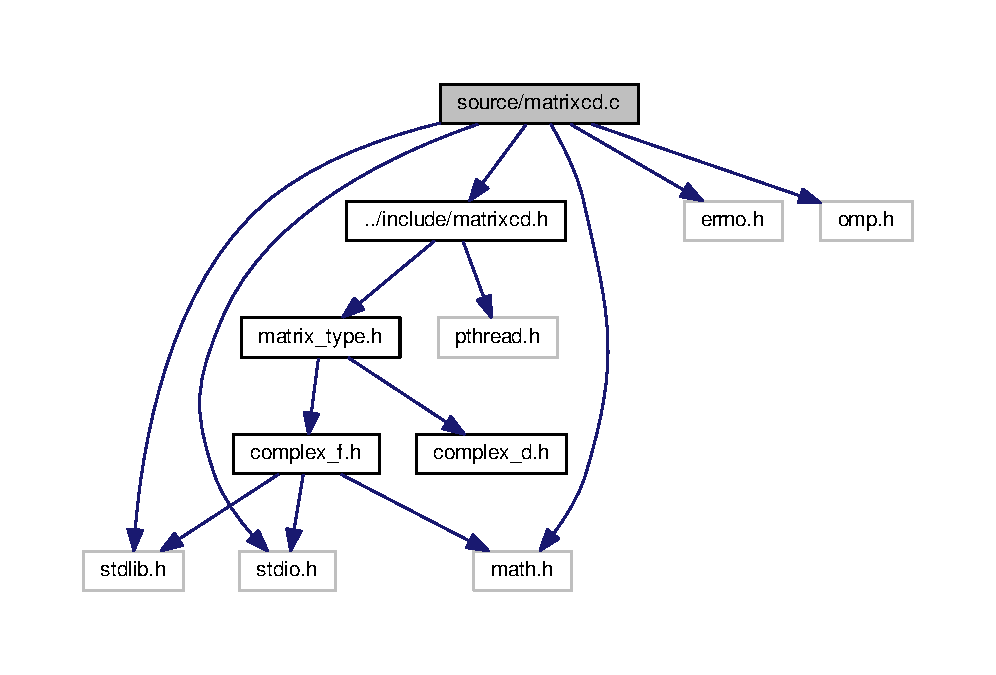
\includegraphics[width=350pt]{matrixcd_8c__incl}
\end{center}
\end{figure}
\subsection*{Functions}
\begin{DoxyCompactItemize}
\item 
void \hyperlink{matrixcd_8c_a8cfe8319ad972882983e40c741bf472e}{print\+Matrix\+CD} (\hyperlink{structMatrix__cd}{Matrix\+\_\+cd} $\ast$a)
\begin{DoxyCompactList}\small\item\em print\+Matrix\+CD display a matrix of \hyperlink{structComplex__d}{Complex\+\_\+d} (usefull for testing) \end{DoxyCompactList}\item 
\hyperlink{structMatrix__cd}{Matrix\+\_\+cd} $\ast$ \hyperlink{matrixcd_8c_a66d35f28fe68c6e02e00028dd65c1d13}{matrix\+Alloc\+CD} (unsigned int rows, unsigned int column)
\begin{DoxyCompactList}\small\item\em matrix\+Alloc\+CD allocate memory for a matrix and initialize it to zero \end{DoxyCompactList}\item 
\hyperlink{structMatrix__cd}{Matrix\+\_\+cd} $\ast$ \hyperlink{matrixcd_8c_aed7ef611733ec971dbfa0e5ac5406ea9}{create\+Random\+Matrix\+CD} (unsigned int rows, unsigned int column)
\begin{DoxyCompactList}\small\item\em create\+Random\+Matrix initialize a random Matrix \end{DoxyCompactList}\item 
void \hyperlink{matrixcd_8c_a5b78f1966b0d2ecf6d3965adc3fcc1cd}{create\+Zero\+Matrix\+CD} (\hyperlink{structMatrix__cd}{Matrix\+\_\+cd} $\ast$J)
\begin{DoxyCompactList}\small\item\em create\+Random\+Matrix initialize a random Matrix \end{DoxyCompactList}\item 
\hyperlink{structMatrix__cd}{Matrix\+\_\+cd} $\ast$ \hyperlink{matrixcd_8c_a9e635491820e7d52dce0d1cadae8fe63}{create\+Test\+Vector\+CD} (unsigned int type)
\begin{DoxyCompactList}\small\item\em create\+Test\+Vector initialize a known vector of size 3\+:1 \end{DoxyCompactList}\item 
void \hyperlink{matrixcd_8c_ae75e700f3b7d09eb844e98f525c2a29e}{create\+Identity\+CD} (\hyperlink{structMatrix__cd}{Matrix\+\_\+cd} $\ast$I)
\begin{DoxyCompactList}\small\item\em create\+Identity\+CD compute the identoty matrix \end{DoxyCompactList}\item 
void \hyperlink{matrixcd_8c_a4cbd12beeab6aaacbf3e4cb467736eed}{free\+Matrix\+CD} (\hyperlink{structMatrix__cd}{Matrix\+\_\+cd} $\ast$A)
\begin{DoxyCompactList}\small\item\em free\+Matrix\+CD free a \hyperlink{structComplex__d}{Complex\+\_\+d} matrix \end{DoxyCompactList}\item 
\hyperlink{structComplex__d}{Complex\+\_\+d} \hyperlink{matrixcd_8c_adaa2d4b812e3ef2108861f30fa328e80}{matrix\+Get\+CD} (\hyperlink{structMatrix__cd}{Matrix\+\_\+cd} $\ast$A, unsigned int i, unsigned int j)
\begin{DoxyCompactList}\small\item\em matrix\+Get\+CD access a specified data of a matrix \end{DoxyCompactList}\item 
void \hyperlink{matrixcd_8c_ac9163e08a5087b566e27cceb5c3c5860}{matrix\+Set\+CD} (\hyperlink{structMatrix__cd}{Matrix\+\_\+cd} $\ast$A, unsigned int i, unsigned int j, const \hyperlink{structComplex__d}{Complex\+\_\+d} c)
\begin{DoxyCompactList}\small\item\em matrix\+Set\+CD set the value of a specified data \end{DoxyCompactList}\item 
void \hyperlink{matrixcd_8c_a665f67f289f63b0dfc0b49a2bb8299e4}{scale\+Matrix\+CD} (\hyperlink{structMatrix__cd}{Matrix\+\_\+cd} $\ast$a, const \hyperlink{structComplex__d}{Complex\+\_\+d} c)
\begin{DoxyCompactList}\small\item\em scale\+Matrix\+CD multiply each data by a constant () \end{DoxyCompactList}\item 
void \hyperlink{matrixcd_8c_a282196989f79b8c5b51bf7f5b06d1a69}{add\+Matrix\+CD} (\hyperlink{structMatrix__cd}{Matrix\+\_\+cd} $\ast$a, \hyperlink{structMatrix__cd}{Matrix\+\_\+cd} $\ast$b)
\begin{DoxyCompactList}\small\item\em add\+Matrix\+CD compute A = A+B \end{DoxyCompactList}\item 
void \hyperlink{matrixcd_8c_a7a10fe5bc61d35cbf5c2e29214ec401e}{add\+Matrix\+T\+CD} (\hyperlink{structMatrix__cd}{Matrix\+\_\+cd} $\ast$a, \hyperlink{structMatrix__cd}{Matrix\+\_\+cd} $\ast$b)
\begin{DoxyCompactList}\small\item\em add\+Matrix\+T\+CD compute A = A+\+BT BT being the transposed matrix of B \end{DoxyCompactList}\item 
void \hyperlink{matrixcd_8c_a1231119363733931d70aac9e36a67f88}{sub\+Matrix\+CD} (\hyperlink{structMatrix__cd}{Matrix\+\_\+cd} $\ast$a, \hyperlink{structMatrix__cd}{Matrix\+\_\+cd} $\ast$b)
\begin{DoxyCompactList}\small\item\em sub\+Matrix\+CD compute A = A-\/B \end{DoxyCompactList}\item 
void \hyperlink{matrixcd_8c_a4a0ff321f98d46e58093a44dc85d08ef}{mul\+Matrix\+CD} (\hyperlink{structMatrix__cd}{Matrix\+\_\+cd} $\ast$a, \hyperlink{structMatrix__cd}{Matrix\+\_\+cd} $\ast$b, \hyperlink{structMatrix__cd}{Matrix\+\_\+cd} $\ast$c)
\begin{DoxyCompactList}\small\item\em compute C = A$\ast$B \end{DoxyCompactList}\item 
void \hyperlink{matrixcd_8c_a0a72a56c77e9fbfc642d7c5687446548}{mat\+Ref\+CD} (\hyperlink{structMatrix__cd}{Matrix\+\_\+cd} $\ast$A)
\begin{DoxyCompactList}\small\item\em mat\+Norm\+CD take the first matrix A value as a reference (ie\+: 1) and scale the other value accoarding to that \end{DoxyCompactList}\item 
void \hyperlink{matrixcd_8c_aa487c335f64ebf80d9c0c0bc8cfbf326}{scale\+Line\+CD} (\hyperlink{structMatrix__cd}{Matrix\+\_\+cd} $\ast$a, unsigned int i, \hyperlink{structComplex__d}{Complex\+\_\+d} f)
\begin{DoxyCompactList}\small\item\em scale\+Line\+CD multiply a line with a \end{DoxyCompactList}\item 
int \hyperlink{matrixcd_8c_ad679b5d98a2361b8e9c03dfc20989d84}{sub\+X\+Lines\+CD} (\hyperlink{structMatrix__cd}{Matrix\+\_\+cd} $\ast$a, unsigned int i, unsigned int i2, \hyperlink{structComplex__d}{Complex\+\_\+d} f)
\begin{DoxyCompactList}\small\item\em sub\+X\+Lines\+CD computes line i -\/ f$\ast$line i2 and store it into line i \end{DoxyCompactList}\item 
void \hyperlink{matrixcd_8c_a47d09cce5e664c00080b5575b8919678}{mul\+Add\+Scale\+Matrix\+CD} (\hyperlink{structMatrix__cd}{Matrix\+\_\+cd} $\ast$result, \hyperlink{structMatrix__cd}{Matrix\+\_\+cd} $\ast$mul1, \hyperlink{structMatrix__cd}{Matrix\+\_\+cd} $\ast$mul2, \hyperlink{structMatrix__cd}{Matrix\+\_\+cd} $\ast$add, \hyperlink{structComplex__d}{Complex\+\_\+d} l, \hyperlink{structComplex__d}{Complex\+\_\+d} s)
\begin{DoxyCompactList}\small\item\em compute result = s$\ast$(mul1$\ast$mul2 + l$\ast$add) \end{DoxyCompactList}\item 
int \hyperlink{matrixcd_8c_aad7adc6a01dfa9d9ec2107abbfed80eb}{is\+Diag\+CD} (\hyperlink{structMatrix__cd}{Matrix\+\_\+cd} $\ast$a)
\begin{DoxyCompactList}\small\item\em checks if the matrix is diagonal and sets its flag if necessary \end{DoxyCompactList}\item 
int \hyperlink{matrixcd_8c_aceb93ede73dda9f4cf4e809d1697a972}{is\+Tri\+U\+CD} (\hyperlink{structMatrix__cd}{Matrix\+\_\+cd} $\ast$a)
\begin{DoxyCompactList}\small\item\em checks if the matrix is triangular UP and sets its flag if necessary \end{DoxyCompactList}\item 
int \hyperlink{matrixcd_8c_a4431b747a67df9288a1fa635746fece4}{is\+Tri\+L\+CD} (\hyperlink{structMatrix__cd}{Matrix\+\_\+cd} $\ast$a)
\begin{DoxyCompactList}\small\item\em checks if the matrix is triangular Low and sets its flag if necessary \end{DoxyCompactList}\item 
int \hyperlink{matrixcd_8c_a23c9874e32512d08db7d97691bb7059b}{is\+Sparse\+CD} (\hyperlink{structMatrix__cd}{Matrix\+\_\+cd} $\ast$a)
\begin{DoxyCompactList}\small\item\em checks if the sparcity of the matrix is superior to 2/3 (allows compression) \end{DoxyCompactList}\end{DoxyCompactItemize}


\subsection{Detailed Description}
to handle matrix operations for complex doubles \begin{DoxyAuthor}{Author}
Nicolas Sourbier 
\end{DoxyAuthor}
\begin{DoxyDate}{Date}
10/09/2018 
\end{DoxyDate}


\subsection{Function Documentation}
\index{matrixcd.\+c@{matrixcd.\+c}!add\+Matrix\+CD@{add\+Matrix\+CD}}
\index{add\+Matrix\+CD@{add\+Matrix\+CD}!matrixcd.\+c@{matrixcd.\+c}}
\subsubsection[{\texorpdfstring{add\+Matrix\+C\+D(\+Matrix\+\_\+cd $\ast$a, Matrix\+\_\+cd $\ast$b)}{addMatrixCD(Matrix_cd *a, Matrix_cd *b)}}]{\setlength{\rightskip}{0pt plus 5cm}void add\+Matrix\+CD (
\begin{DoxyParamCaption}
\item[{{\bf Matrix\+\_\+cd} $\ast$}]{a, }
\item[{{\bf Matrix\+\_\+cd} $\ast$}]{b}
\end{DoxyParamCaption}
)}\hypertarget{matrixcd_8c_a282196989f79b8c5b51bf7f5b06d1a69}{}\label{matrixcd_8c_a282196989f79b8c5b51bf7f5b06d1a69}


add\+Matrix\+CD compute A = A+B 


\begin{DoxyParams}{Parameters}
{\em a} & matrix \\
\hline
{\em b} & matrix \\
\hline
\end{DoxyParams}
\index{matrixcd.\+c@{matrixcd.\+c}!add\+Matrix\+T\+CD@{add\+Matrix\+T\+CD}}
\index{add\+Matrix\+T\+CD@{add\+Matrix\+T\+CD}!matrixcd.\+c@{matrixcd.\+c}}
\subsubsection[{\texorpdfstring{add\+Matrix\+T\+C\+D(\+Matrix\+\_\+cd $\ast$a, Matrix\+\_\+cd $\ast$b)}{addMatrixTCD(Matrix_cd *a, Matrix_cd *b)}}]{\setlength{\rightskip}{0pt plus 5cm}void add\+Matrix\+T\+CD (
\begin{DoxyParamCaption}
\item[{{\bf Matrix\+\_\+cd} $\ast$}]{a, }
\item[{{\bf Matrix\+\_\+cd} $\ast$}]{b}
\end{DoxyParamCaption}
)}\hypertarget{matrixcd_8c_a7a10fe5bc61d35cbf5c2e29214ec401e}{}\label{matrixcd_8c_a7a10fe5bc61d35cbf5c2e29214ec401e}


add\+Matrix\+T\+CD compute A = A+\+BT BT being the transposed matrix of B 


\begin{DoxyParams}{Parameters}
{\em a} & matrix \\
\hline
{\em b} & matrix \\
\hline
\end{DoxyParams}
\index{matrixcd.\+c@{matrixcd.\+c}!create\+Identity\+CD@{create\+Identity\+CD}}
\index{create\+Identity\+CD@{create\+Identity\+CD}!matrixcd.\+c@{matrixcd.\+c}}
\subsubsection[{\texorpdfstring{create\+Identity\+C\+D(\+Matrix\+\_\+cd $\ast$\+I)}{createIdentityCD(Matrix_cd *I)}}]{\setlength{\rightskip}{0pt plus 5cm}void create\+Identity\+CD (
\begin{DoxyParamCaption}
\item[{{\bf Matrix\+\_\+cd} $\ast$}]{id}
\end{DoxyParamCaption}
)}\hypertarget{matrixcd_8c_ae75e700f3b7d09eb844e98f525c2a29e}{}\label{matrixcd_8c_ae75e700f3b7d09eb844e98f525c2a29e}


create\+Identity\+CD compute the identoty matrix 


\begin{DoxyParams}{Parameters}
{\em id} & A pointer to store the result \\
\hline
\end{DoxyParams}
\index{matrixcd.\+c@{matrixcd.\+c}!create\+Random\+Matrix\+CD@{create\+Random\+Matrix\+CD}}
\index{create\+Random\+Matrix\+CD@{create\+Random\+Matrix\+CD}!matrixcd.\+c@{matrixcd.\+c}}
\subsubsection[{\texorpdfstring{create\+Random\+Matrix\+C\+D(unsigned int rows, unsigned int column)}{createRandomMatrixCD(unsigned int rows, unsigned int column)}}]{\setlength{\rightskip}{0pt plus 5cm}{\bf Matrix\+\_\+cd}$\ast$ create\+Random\+Matrix\+CD (
\begin{DoxyParamCaption}
\item[{unsigned int}]{rows, }
\item[{unsigned int}]{column}
\end{DoxyParamCaption}
)}\hypertarget{matrixcd_8c_aed7ef611733ec971dbfa0e5ac5406ea9}{}\label{matrixcd_8c_aed7ef611733ec971dbfa0e5ac5406ea9}


create\+Random\+Matrix initialize a random Matrix 


\begin{DoxyParams}{Parameters}
{\em rows} & number of rows \\
\hline
{\em column} & number of columns \\
\hline
\end{DoxyParams}
\begin{DoxyReturn}{Returns}
the random matrix 
\end{DoxyReturn}
\index{matrixcd.\+c@{matrixcd.\+c}!create\+Test\+Vector\+CD@{create\+Test\+Vector\+CD}}
\index{create\+Test\+Vector\+CD@{create\+Test\+Vector\+CD}!matrixcd.\+c@{matrixcd.\+c}}
\subsubsection[{\texorpdfstring{create\+Test\+Vector\+C\+D(unsigned int type)}{createTestVectorCD(unsigned int type)}}]{\setlength{\rightskip}{0pt plus 5cm}{\bf Matrix\+\_\+cd}$\ast$ create\+Test\+Vector\+CD (
\begin{DoxyParamCaption}
\item[{unsigned int}]{type}
\end{DoxyParamCaption}
)}\hypertarget{matrixcd_8c_a9e635491820e7d52dce0d1cadae8fe63}{}\label{matrixcd_8c_a9e635491820e7d52dce0d1cadae8fe63}


create\+Test\+Vector initialize a known vector of size 3\+:1 


\begin{DoxyParams}{Parameters}
{\em type} & (1 or 2) you\textquotesingle{}ve got choice between two test vectors \\
\hline
\end{DoxyParams}
\begin{DoxyReturn}{Returns}
the random matrix 
\end{DoxyReturn}
\index{matrixcd.\+c@{matrixcd.\+c}!create\+Zero\+Matrix\+CD@{create\+Zero\+Matrix\+CD}}
\index{create\+Zero\+Matrix\+CD@{create\+Zero\+Matrix\+CD}!matrixcd.\+c@{matrixcd.\+c}}
\subsubsection[{\texorpdfstring{create\+Zero\+Matrix\+C\+D(\+Matrix\+\_\+cd $\ast$\+J)}{createZeroMatrixCD(Matrix_cd *J)}}]{\setlength{\rightskip}{0pt plus 5cm}void create\+Zero\+Matrix\+CD (
\begin{DoxyParamCaption}
\item[{{\bf Matrix\+\_\+cd} $\ast$}]{J}
\end{DoxyParamCaption}
)}\hypertarget{matrixcd_8c_a5b78f1966b0d2ecf6d3965adc3fcc1cd}{}\label{matrixcd_8c_a5b78f1966b0d2ecf6d3965adc3fcc1cd}


create\+Random\+Matrix initialize a random Matrix 


\begin{DoxyParams}{Parameters}
{\em J} & a matrix to fill with zeros \\
\hline
\end{DoxyParams}
\begin{DoxyReturn}{Returns}
the random matrix 
\end{DoxyReturn}
\index{matrixcd.\+c@{matrixcd.\+c}!free\+Matrix\+CD@{free\+Matrix\+CD}}
\index{free\+Matrix\+CD@{free\+Matrix\+CD}!matrixcd.\+c@{matrixcd.\+c}}
\subsubsection[{\texorpdfstring{free\+Matrix\+C\+D(\+Matrix\+\_\+cd $\ast$\+A)}{freeMatrixCD(Matrix_cd *A)}}]{\setlength{\rightskip}{0pt plus 5cm}void free\+Matrix\+CD (
\begin{DoxyParamCaption}
\item[{{\bf Matrix\+\_\+cd} $\ast$}]{A}
\end{DoxyParamCaption}
)}\hypertarget{matrixcd_8c_a4cbd12beeab6aaacbf3e4cb467736eed}{}\label{matrixcd_8c_a4cbd12beeab6aaacbf3e4cb467736eed}


free\+Matrix\+CD free a \hyperlink{structComplex__d}{Complex\+\_\+d} matrix 


\begin{DoxyParams}{Parameters}
{\em A} & the matrix to free \\
\hline
\end{DoxyParams}
\index{matrixcd.\+c@{matrixcd.\+c}!is\+Diag\+CD@{is\+Diag\+CD}}
\index{is\+Diag\+CD@{is\+Diag\+CD}!matrixcd.\+c@{matrixcd.\+c}}
\subsubsection[{\texorpdfstring{is\+Diag\+C\+D(\+Matrix\+\_\+cd $\ast$a)}{isDiagCD(Matrix_cd *a)}}]{\setlength{\rightskip}{0pt plus 5cm}int is\+Diag\+CD (
\begin{DoxyParamCaption}
\item[{{\bf Matrix\+\_\+cd} $\ast$}]{a}
\end{DoxyParamCaption}
)}\hypertarget{matrixcd_8c_aad7adc6a01dfa9d9ec2107abbfed80eb}{}\label{matrixcd_8c_aad7adc6a01dfa9d9ec2107abbfed80eb}


checks if the matrix is diagonal and sets its flag if necessary 


\begin{DoxyParams}{Parameters}
{\em a} & the matrix to test returns 1 if diag, 0 otherwise \\
\hline
\end{DoxyParams}
\index{matrixcd.\+c@{matrixcd.\+c}!is\+Sparse\+CD@{is\+Sparse\+CD}}
\index{is\+Sparse\+CD@{is\+Sparse\+CD}!matrixcd.\+c@{matrixcd.\+c}}
\subsubsection[{\texorpdfstring{is\+Sparse\+C\+D(\+Matrix\+\_\+cd $\ast$a)}{isSparseCD(Matrix_cd *a)}}]{\setlength{\rightskip}{0pt plus 5cm}int is\+Sparse\+CD (
\begin{DoxyParamCaption}
\item[{{\bf Matrix\+\_\+cd} $\ast$}]{a}
\end{DoxyParamCaption}
)}\hypertarget{matrixcd_8c_a23c9874e32512d08db7d97691bb7059b}{}\label{matrixcd_8c_a23c9874e32512d08db7d97691bb7059b}


checks if the sparcity of the matrix is superior to 2/3 (allows compression) 


\begin{DoxyParams}{Parameters}
{\em a} & the matrix to test returns 1 if diag, 0 otherwise \\
\hline
\end{DoxyParams}
\index{matrixcd.\+c@{matrixcd.\+c}!is\+Tri\+L\+CD@{is\+Tri\+L\+CD}}
\index{is\+Tri\+L\+CD@{is\+Tri\+L\+CD}!matrixcd.\+c@{matrixcd.\+c}}
\subsubsection[{\texorpdfstring{is\+Tri\+L\+C\+D(\+Matrix\+\_\+cd $\ast$a)}{isTriLCD(Matrix_cd *a)}}]{\setlength{\rightskip}{0pt plus 5cm}int is\+Tri\+L\+CD (
\begin{DoxyParamCaption}
\item[{{\bf Matrix\+\_\+cd} $\ast$}]{a}
\end{DoxyParamCaption}
)}\hypertarget{matrixcd_8c_a4431b747a67df9288a1fa635746fece4}{}\label{matrixcd_8c_a4431b747a67df9288a1fa635746fece4}


checks if the matrix is triangular Low and sets its flag if necessary 


\begin{DoxyParams}{Parameters}
{\em a} & the matrix to test returns 1 if diag, 0 otherwise \\
\hline
\end{DoxyParams}
\index{matrixcd.\+c@{matrixcd.\+c}!is\+Tri\+U\+CD@{is\+Tri\+U\+CD}}
\index{is\+Tri\+U\+CD@{is\+Tri\+U\+CD}!matrixcd.\+c@{matrixcd.\+c}}
\subsubsection[{\texorpdfstring{is\+Tri\+U\+C\+D(\+Matrix\+\_\+cd $\ast$a)}{isTriUCD(Matrix_cd *a)}}]{\setlength{\rightskip}{0pt plus 5cm}int is\+Tri\+U\+CD (
\begin{DoxyParamCaption}
\item[{{\bf Matrix\+\_\+cd} $\ast$}]{a}
\end{DoxyParamCaption}
)}\hypertarget{matrixcd_8c_aceb93ede73dda9f4cf4e809d1697a972}{}\label{matrixcd_8c_aceb93ede73dda9f4cf4e809d1697a972}


checks if the matrix is triangular UP and sets its flag if necessary 


\begin{DoxyParams}{Parameters}
{\em a} & the matrix to test returns 1 if diag, 0 otherwise \\
\hline
\end{DoxyParams}
\index{matrixcd.\+c@{matrixcd.\+c}!mat\+Ref\+CD@{mat\+Ref\+CD}}
\index{mat\+Ref\+CD@{mat\+Ref\+CD}!matrixcd.\+c@{matrixcd.\+c}}
\subsubsection[{\texorpdfstring{mat\+Ref\+C\+D(\+Matrix\+\_\+cd $\ast$\+A)}{matRefCD(Matrix_cd *A)}}]{\setlength{\rightskip}{0pt plus 5cm}void mat\+Ref\+CD (
\begin{DoxyParamCaption}
\item[{{\bf Matrix\+\_\+cd} $\ast$}]{A}
\end{DoxyParamCaption}
)}\hypertarget{matrixcd_8c_a0a72a56c77e9fbfc642d7c5687446548}{}\label{matrixcd_8c_a0a72a56c77e9fbfc642d7c5687446548}


mat\+Norm\+CD take the first matrix A value as a reference (ie\+: 1) and scale the other value accoarding to that 


\begin{DoxyParams}{Parameters}
{\em A} & the matrix that we want to \char`\"{}norm\char`\"{} \\
\hline
\end{DoxyParams}
\index{matrixcd.\+c@{matrixcd.\+c}!matrix\+Alloc\+CD@{matrix\+Alloc\+CD}}
\index{matrix\+Alloc\+CD@{matrix\+Alloc\+CD}!matrixcd.\+c@{matrixcd.\+c}}
\subsubsection[{\texorpdfstring{matrix\+Alloc\+C\+D(unsigned int rows, unsigned int column)}{matrixAllocCD(unsigned int rows, unsigned int column)}}]{\setlength{\rightskip}{0pt plus 5cm}{\bf Matrix\+\_\+cd}$\ast$ matrix\+Alloc\+CD (
\begin{DoxyParamCaption}
\item[{unsigned int}]{rows, }
\item[{unsigned int}]{column}
\end{DoxyParamCaption}
)}\hypertarget{matrixcd_8c_a66d35f28fe68c6e02e00028dd65c1d13}{}\label{matrixcd_8c_a66d35f28fe68c6e02e00028dd65c1d13}


matrix\+Alloc\+CD allocate memory for a matrix and initialize it to zero 


\begin{DoxyParams}{Parameters}
{\em rows} & number of rows \\
\hline
{\em column} & number of columns \\
\hline
\end{DoxyParams}
\begin{DoxyReturn}{Returns}
the allocated matrix if no errors occured, N\+U\+LL if not 
\end{DoxyReturn}
\index{matrixcd.\+c@{matrixcd.\+c}!matrix\+Get\+CD@{matrix\+Get\+CD}}
\index{matrix\+Get\+CD@{matrix\+Get\+CD}!matrixcd.\+c@{matrixcd.\+c}}
\subsubsection[{\texorpdfstring{matrix\+Get\+C\+D(\+Matrix\+\_\+cd $\ast$\+A, unsigned int i, unsigned int j)}{matrixGetCD(Matrix_cd *A, unsigned int i, unsigned int j)}}]{\setlength{\rightskip}{0pt plus 5cm}{\bf Complex\+\_\+d} matrix\+Get\+CD (
\begin{DoxyParamCaption}
\item[{{\bf Matrix\+\_\+cd} $\ast$}]{A, }
\item[{unsigned int}]{i, }
\item[{unsigned int}]{j}
\end{DoxyParamCaption}
)}\hypertarget{matrixcd_8c_adaa2d4b812e3ef2108861f30fa328e80}{}\label{matrixcd_8c_adaa2d4b812e3ef2108861f30fa328e80}


matrix\+Get\+CD access a specified data of a matrix 


\begin{DoxyParams}{Parameters}
{\em A} & the matrix \\
\hline
{\em i} & the index of rows \\
\hline
{\em j} & the index on columns \\
\hline
\end{DoxyParams}
\begin{DoxyReturn}{Returns}
the data A(i,j) 
\end{DoxyReturn}
\begin{DoxyWarning}{Warning}
if the matrix in parameter is N\+U\+LL, returns 0 
\end{DoxyWarning}
\index{matrixcd.\+c@{matrixcd.\+c}!matrix\+Set\+CD@{matrix\+Set\+CD}}
\index{matrix\+Set\+CD@{matrix\+Set\+CD}!matrixcd.\+c@{matrixcd.\+c}}
\subsubsection[{\texorpdfstring{matrix\+Set\+C\+D(\+Matrix\+\_\+cd $\ast$\+A, unsigned int i, unsigned int j, const Complex\+\_\+d c)}{matrixSetCD(Matrix_cd *A, unsigned int i, unsigned int j, const Complex_d c)}}]{\setlength{\rightskip}{0pt plus 5cm}void matrix\+Set\+CD (
\begin{DoxyParamCaption}
\item[{{\bf Matrix\+\_\+cd} $\ast$}]{A, }
\item[{unsigned int}]{i, }
\item[{unsigned int}]{j, }
\item[{const {\bf Complex\+\_\+d}}]{c}
\end{DoxyParamCaption}
)}\hypertarget{matrixcd_8c_ac9163e08a5087b566e27cceb5c3c5860}{}\label{matrixcd_8c_ac9163e08a5087b566e27cceb5c3c5860}


matrix\+Set\+CD set the value of a specified data 


\begin{DoxyParams}{Parameters}
{\em A} & the matrix \\
\hline
{\em i} & the index on rows \\
\hline
{\em j} & the index on columns \\
\hline
{\em c} & the to set at A(i,j) \\
\hline
\end{DoxyParams}
\index{matrixcd.\+c@{matrixcd.\+c}!mul\+Add\+Scale\+Matrix\+CD@{mul\+Add\+Scale\+Matrix\+CD}}
\index{mul\+Add\+Scale\+Matrix\+CD@{mul\+Add\+Scale\+Matrix\+CD}!matrixcd.\+c@{matrixcd.\+c}}
\subsubsection[{\texorpdfstring{mul\+Add\+Scale\+Matrix\+C\+D(\+Matrix\+\_\+cd $\ast$result, Matrix\+\_\+cd $\ast$mul1, Matrix\+\_\+cd $\ast$mul2, Matrix\+\_\+cd $\ast$add, Complex\+\_\+d l, Complex\+\_\+d s)}{mulAddScaleMatrixCD(Matrix_cd *result, Matrix_cd *mul1, Matrix_cd *mul2, Matrix_cd *add, Complex_d l, Complex_d s)}}]{\setlength{\rightskip}{0pt plus 5cm}void mul\+Add\+Scale\+Matrix\+CD (
\begin{DoxyParamCaption}
\item[{{\bf Matrix\+\_\+cd} $\ast$}]{result, }
\item[{{\bf Matrix\+\_\+cd} $\ast$}]{mul1, }
\item[{{\bf Matrix\+\_\+cd} $\ast$}]{mul2, }
\item[{{\bf Matrix\+\_\+cd} $\ast$}]{add, }
\item[{{\bf Complex\+\_\+d}}]{l, }
\item[{{\bf Complex\+\_\+d}}]{s}
\end{DoxyParamCaption}
)}\hypertarget{matrixcd_8c_a47d09cce5e664c00080b5575b8919678}{}\label{matrixcd_8c_a47d09cce5e664c00080b5575b8919678}


compute result = s$\ast$(mul1$\ast$mul2 + l$\ast$add) 


\begin{DoxyParams}{Parameters}
{\em result} & a matrix to store the result \\
\hline
{\em mul1} & \& \\
\hline
{\em mul2} & matrices to multiply \\
\hline
{\em add} & a matrix to add to the previous product \\
\hline
{\em l} & a \hyperlink{structComplex__d}{Complex\+\_\+d} to scale the add matrix \\
\hline
{\em s} & a \hyperlink{structComplex__d}{Complex\+\_\+d} to scale the result doesn\textquotesingle{}t use optimisations related to the matrix properties \\
\hline
\end{DoxyParams}
\index{matrixcd.\+c@{matrixcd.\+c}!mul\+Matrix\+CD@{mul\+Matrix\+CD}}
\index{mul\+Matrix\+CD@{mul\+Matrix\+CD}!matrixcd.\+c@{matrixcd.\+c}}
\subsubsection[{\texorpdfstring{mul\+Matrix\+C\+D(\+Matrix\+\_\+cd $\ast$a, Matrix\+\_\+cd $\ast$b, Matrix\+\_\+cd $\ast$c)}{mulMatrixCD(Matrix_cd *a, Matrix_cd *b, Matrix_cd *c)}}]{\setlength{\rightskip}{0pt plus 5cm}void mul\+Matrix\+CD (
\begin{DoxyParamCaption}
\item[{{\bf Matrix\+\_\+cd} $\ast$}]{a, }
\item[{{\bf Matrix\+\_\+cd} $\ast$}]{b, }
\item[{{\bf Matrix\+\_\+cd} $\ast$}]{c}
\end{DoxyParamCaption}
)}\hypertarget{matrixcd_8c_a4a0ff321f98d46e58093a44dc85d08ef}{}\label{matrixcd_8c_a4a0ff321f98d46e58093a44dc85d08ef}


compute C = A$\ast$B 


\begin{DoxyParams}{Parameters}
{\em a} & matrix \\
\hline
{\em b} & matrix \\
\hline
{\em c} & a matrix to store the result \\
\hline
\end{DoxyParams}
\index{matrixcd.\+c@{matrixcd.\+c}!print\+Matrix\+CD@{print\+Matrix\+CD}}
\index{print\+Matrix\+CD@{print\+Matrix\+CD}!matrixcd.\+c@{matrixcd.\+c}}
\subsubsection[{\texorpdfstring{print\+Matrix\+C\+D(\+Matrix\+\_\+cd $\ast$a)}{printMatrixCD(Matrix_cd *a)}}]{\setlength{\rightskip}{0pt plus 5cm}void print\+Matrix\+CD (
\begin{DoxyParamCaption}
\item[{{\bf Matrix\+\_\+cd} $\ast$}]{a}
\end{DoxyParamCaption}
)}\hypertarget{matrixcd_8c_a8cfe8319ad972882983e40c741bf472e}{}\label{matrixcd_8c_a8cfe8319ad972882983e40c741bf472e}


print\+Matrix\+CD display a matrix of \hyperlink{structComplex__d}{Complex\+\_\+d} (usefull for testing) 


\begin{DoxyParams}{Parameters}
{\em a} & the matrix to display \\
\hline
\end{DoxyParams}
\index{matrixcd.\+c@{matrixcd.\+c}!scale\+Line\+CD@{scale\+Line\+CD}}
\index{scale\+Line\+CD@{scale\+Line\+CD}!matrixcd.\+c@{matrixcd.\+c}}
\subsubsection[{\texorpdfstring{scale\+Line\+C\+D(\+Matrix\+\_\+cd $\ast$a, unsigned int i, Complex\+\_\+d f)}{scaleLineCD(Matrix_cd *a, unsigned int i, Complex_d f)}}]{\setlength{\rightskip}{0pt plus 5cm}void scale\+Line\+CD (
\begin{DoxyParamCaption}
\item[{{\bf Matrix\+\_\+cd} $\ast$}]{a, }
\item[{unsigned int}]{i, }
\item[{{\bf Complex\+\_\+d}}]{f}
\end{DoxyParamCaption}
)}\hypertarget{matrixcd_8c_aa487c335f64ebf80d9c0c0bc8cfbf326}{}\label{matrixcd_8c_aa487c335f64ebf80d9c0c0bc8cfbf326}


scale\+Line\+CD multiply a line with a 


\begin{DoxyParams}{Parameters}
{\em a} & the matrix \\
\hline
{\em i} & the index of the line we want to scale \\
\hline
{\em f} & the that will scale the line \\
\hline
\end{DoxyParams}
\index{matrixcd.\+c@{matrixcd.\+c}!scale\+Matrix\+CD@{scale\+Matrix\+CD}}
\index{scale\+Matrix\+CD@{scale\+Matrix\+CD}!matrixcd.\+c@{matrixcd.\+c}}
\subsubsection[{\texorpdfstring{scale\+Matrix\+C\+D(\+Matrix\+\_\+cd $\ast$a, const Complex\+\_\+d c)}{scaleMatrixCD(Matrix_cd *a, const Complex_d c)}}]{\setlength{\rightskip}{0pt plus 5cm}void scale\+Matrix\+CD (
\begin{DoxyParamCaption}
\item[{{\bf Matrix\+\_\+cd} $\ast$}]{a, }
\item[{const {\bf Complex\+\_\+d}}]{c}
\end{DoxyParamCaption}
)}\hypertarget{matrixcd_8c_a665f67f289f63b0dfc0b49a2bb8299e4}{}\label{matrixcd_8c_a665f67f289f63b0dfc0b49a2bb8299e4}


scale\+Matrix\+CD multiply each data by a constant () 


\begin{DoxyParams}{Parameters}
{\em a} & the matrix to scale \\
\hline
{\em c} & the \\
\hline
\end{DoxyParams}
\index{matrixcd.\+c@{matrixcd.\+c}!sub\+Matrix\+CD@{sub\+Matrix\+CD}}
\index{sub\+Matrix\+CD@{sub\+Matrix\+CD}!matrixcd.\+c@{matrixcd.\+c}}
\subsubsection[{\texorpdfstring{sub\+Matrix\+C\+D(\+Matrix\+\_\+cd $\ast$a, Matrix\+\_\+cd $\ast$b)}{subMatrixCD(Matrix_cd *a, Matrix_cd *b)}}]{\setlength{\rightskip}{0pt plus 5cm}void sub\+Matrix\+CD (
\begin{DoxyParamCaption}
\item[{{\bf Matrix\+\_\+cd} $\ast$}]{a, }
\item[{{\bf Matrix\+\_\+cd} $\ast$}]{b}
\end{DoxyParamCaption}
)}\hypertarget{matrixcd_8c_a1231119363733931d70aac9e36a67f88}{}\label{matrixcd_8c_a1231119363733931d70aac9e36a67f88}


sub\+Matrix\+CD compute A = A-\/B 


\begin{DoxyParams}{Parameters}
{\em a} & matrix \\
\hline
{\em b} & matrix \\
\hline
\end{DoxyParams}
\index{matrixcd.\+c@{matrixcd.\+c}!sub\+X\+Lines\+CD@{sub\+X\+Lines\+CD}}
\index{sub\+X\+Lines\+CD@{sub\+X\+Lines\+CD}!matrixcd.\+c@{matrixcd.\+c}}
\subsubsection[{\texorpdfstring{sub\+X\+Lines\+C\+D(\+Matrix\+\_\+cd $\ast$a, unsigned int i, unsigned int i2, Complex\+\_\+d f)}{subXLinesCD(Matrix_cd *a, unsigned int i, unsigned int i2, Complex_d f)}}]{\setlength{\rightskip}{0pt plus 5cm}int sub\+X\+Lines\+CD (
\begin{DoxyParamCaption}
\item[{{\bf Matrix\+\_\+cd} $\ast$}]{a, }
\item[{unsigned int}]{i, }
\item[{unsigned int}]{i2, }
\item[{{\bf Complex\+\_\+d}}]{f}
\end{DoxyParamCaption}
)}\hypertarget{matrixcd_8c_ad679b5d98a2361b8e9c03dfc20989d84}{}\label{matrixcd_8c_ad679b5d98a2361b8e9c03dfc20989d84}


sub\+X\+Lines\+CD computes line i -\/ f$\ast$line i2 and store it into line i 


\begin{DoxyParams}{Parameters}
{\em a} & the matrix \\
\hline
{\em i} & the index of the line to update \\
\hline
{\em i2} & the index of the \char`\"{}reference\char`\"{} line \\
\hline
{\em f} & a to scale the matrix \\
\hline
\end{DoxyParams}

\hypertarget{matrixcf_8c}{}\section{matrixcf.\+c File Reference}
\label{matrixcf_8c}\index{matrixcf.\+c@{matrixcf.\+c}}
{\ttfamily \#include $<$stdlib.\+h$>$}\\*
{\ttfamily \#include $<$stdio.\+h$>$}\\*
{\ttfamily \#include $<$math.\+h$>$}\\*
{\ttfamily \#include \char`\"{}matrixcf.\+h\char`\"{}}\\*
{\ttfamily \#include \char`\"{}errno.\+h\char`\"{}}\\*
{\ttfamily \#include $<$omp.\+h$>$}\\*
Include dependency graph for matrixcf.\+c\+:\nopagebreak
\begin{figure}[H]
\begin{center}
\leavevmode
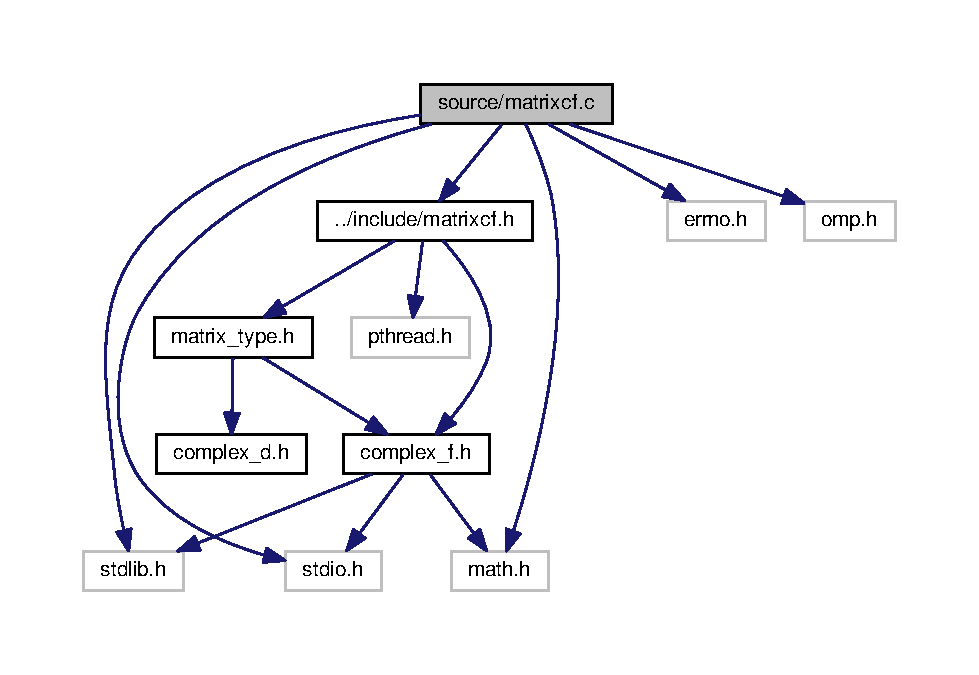
\includegraphics[width=350pt]{matrixcf_8c__incl}
\end{center}
\end{figure}
\subsection*{Functions}
\begin{DoxyCompactItemize}
\item 
void \hyperlink{matrixcf_8c_a442e1077e0c8060c0fdb9f86de1534a9}{print\+Matrix\+CF} (\hyperlink{structMatrix__cf}{Matrix\+\_\+cf} $\ast$a)
\begin{DoxyCompactList}\small\item\em print\+Matrix\+CF display a matrix of \hyperlink{structComplex__f}{Complex\+\_\+f} (usefull for testing) \end{DoxyCompactList}\item 
\hyperlink{structMatrix__cf}{Matrix\+\_\+cf} $\ast$ \hyperlink{matrixcf_8c_a39e7a96197ea705a3691639ce475f5a5}{matrix\+Alloc\+CF} (unsigned int rows, unsigned int column)
\begin{DoxyCompactList}\small\item\em matrix\+Alloc\+CF allocate memory for a matrix and initialize it to zero \end{DoxyCompactList}\item 
\hyperlink{structMatrix__cf}{Matrix\+\_\+cf} $\ast$ \hyperlink{matrixcf_8c_a8db1179a10a7f134d7c63397a6c031b1}{create\+Random\+Matrix\+CF} (unsigned int rows, unsigned int column)
\begin{DoxyCompactList}\small\item\em create\+Random\+Matrix initialize a random Matrix \end{DoxyCompactList}\item 
void \hyperlink{matrixcf_8c_a3d6e512a8597edac8d6d060da8dce93b}{create\+Zero\+Matrix\+CF} (\hyperlink{structMatrix__cf}{Matrix\+\_\+cf} $\ast$J)
\begin{DoxyCompactList}\small\item\em create\+Random\+Matrix initialize a random Matrix \end{DoxyCompactList}\item 
\hyperlink{structMatrix__cf}{Matrix\+\_\+cf} $\ast$ \hyperlink{matrixcf_8c_a8856240cb751ea0059fd0a493f40e358}{create\+Test\+Vector\+CF} (unsigned int type)
\begin{DoxyCompactList}\small\item\em create\+Test\+Vector initialize a known vector of size 3\+:1 \end{DoxyCompactList}\item 
void \hyperlink{matrixcf_8c_ac0c72559d97199f25cda818c603005d4}{create\+Identity\+CF} (\hyperlink{structMatrix__cf}{Matrix\+\_\+cf} $\ast$I)
\begin{DoxyCompactList}\small\item\em create\+Identity\+CF compute the identoty matrix \end{DoxyCompactList}\item 
void \hyperlink{matrixcf_8c_a3dc1b7b64de877b4c5ed94e77faef6b5}{free\+Matrix\+CF} (\hyperlink{structMatrix__cf}{Matrix\+\_\+cf} $\ast$A)
\begin{DoxyCompactList}\small\item\em free\+Matrix\+CF free a \hyperlink{structComplex__f}{Complex\+\_\+f} matrix \end{DoxyCompactList}\item 
\hyperlink{structComplex__f}{Complex\+\_\+f} \hyperlink{matrixcf_8c_ae9ce7ec96f11928ce01ac46edaacf09b}{matrix\+Get\+CF} (\hyperlink{structMatrix__cf}{Matrix\+\_\+cf} $\ast$A, unsigned int i, unsigned int j)
\begin{DoxyCompactList}\small\item\em matrix\+Get\+CF access a specified data of a matrix \end{DoxyCompactList}\item 
void \hyperlink{matrixcf_8c_abb32dd6231976a0dbda098df6dd3386f}{matrix\+Set\+CF} (\hyperlink{structMatrix__cf}{Matrix\+\_\+cf} $\ast$A, unsigned int i, unsigned int j, const \hyperlink{structComplex__f}{Complex\+\_\+f} c)
\begin{DoxyCompactList}\small\item\em matrix\+Set\+CF set the value of a specified data \end{DoxyCompactList}\item 
void \hyperlink{matrixcf_8c_a4ed28ec9b93a048f236a5440dd126dad}{scale\+Matrix\+CF} (\hyperlink{structMatrix__cf}{Matrix\+\_\+cf} $\ast$a, const \hyperlink{structComplex__f}{Complex\+\_\+f} c)
\begin{DoxyCompactList}\small\item\em scale\+Matrix\+CF multiply each data by a constant () \end{DoxyCompactList}\item 
void \hyperlink{matrixcf_8c_a23d12aacfcc8c0c22953955b9de082a3}{add\+Matrix\+CF} (\hyperlink{structMatrix__cf}{Matrix\+\_\+cf} $\ast$a, \hyperlink{structMatrix__cf}{Matrix\+\_\+cf} $\ast$b)
\begin{DoxyCompactList}\small\item\em add\+Matrix\+CF compute A = A+B \end{DoxyCompactList}\item 
void \hyperlink{matrixcf_8c_acb2f4bca1c5a589a83dd21b0847de0f7}{add\+Matrix\+T\+CF} (\hyperlink{structMatrix__cf}{Matrix\+\_\+cf} $\ast$a, \hyperlink{structMatrix__cf}{Matrix\+\_\+cf} $\ast$b)
\begin{DoxyCompactList}\small\item\em add\+Matrix\+T\+CF compute A = A+\+BT BT being the transposed matrix of B \end{DoxyCompactList}\item 
void \hyperlink{matrixcf_8c_a94030ea97022060031fe3bd7b19fb507}{sub\+Matrix\+CF} (\hyperlink{structMatrix__cf}{Matrix\+\_\+cf} $\ast$a, \hyperlink{structMatrix__cf}{Matrix\+\_\+cf} $\ast$b)
\begin{DoxyCompactList}\small\item\em sub\+Matrix\+CF compute A = A-\/B \end{DoxyCompactList}\item 
void \hyperlink{matrixcf_8c_a9c7a762d9828fdf2b62075ed047f448b}{mul\+Matrix\+CF} (\hyperlink{structMatrix__cf}{Matrix\+\_\+cf} $\ast$a, \hyperlink{structMatrix__cf}{Matrix\+\_\+cf} $\ast$b, \hyperlink{structMatrix__cf}{Matrix\+\_\+cf} $\ast$c)
\begin{DoxyCompactList}\small\item\em compute C = A$\ast$B \end{DoxyCompactList}\item 
void \hyperlink{matrixcf_8c_ad81900663e5a729a4d887adee1c84988}{mat\+Ref\+CF} (\hyperlink{structMatrix__cf}{Matrix\+\_\+cf} $\ast$A)
\begin{DoxyCompactList}\small\item\em mat\+Norm\+CF take the first matrix A value as a reference (ie\+: 1) and scale the other value accoarding to that \end{DoxyCompactList}\item 
void \hyperlink{matrixcf_8c_aa44e9f047fc84250a45cbf3a3764f82a}{scale\+Line\+CF} (\hyperlink{structMatrix__cf}{Matrix\+\_\+cf} $\ast$a, unsigned int i, \hyperlink{structComplex__f}{Complex\+\_\+f} f)
\begin{DoxyCompactList}\small\item\em scale\+Line\+CF multiply a line with a \end{DoxyCompactList}\item 
int \hyperlink{matrixcf_8c_aeb31172c90e1dcb05d800c882edc56b3}{sub\+X\+Lines\+CF} (\hyperlink{structMatrix__cf}{Matrix\+\_\+cf} $\ast$a, unsigned int i, unsigned int i2, \hyperlink{structComplex__f}{Complex\+\_\+f} f)
\begin{DoxyCompactList}\small\item\em sub\+X\+Lines\+CF computes line i -\/ f$\ast$line i2 and store it into line i \end{DoxyCompactList}\item 
void \hyperlink{matrixcf_8c_a5cef9887dfd2d47c071cd3f31c675a02}{mul\+Add\+Scale\+Matrix\+CF} (\hyperlink{structMatrix__cf}{Matrix\+\_\+cf} $\ast$result, \hyperlink{structMatrix__cf}{Matrix\+\_\+cf} $\ast$mul1, \hyperlink{structMatrix__cf}{Matrix\+\_\+cf} $\ast$mul2, \hyperlink{structMatrix__cf}{Matrix\+\_\+cf} $\ast$add, \hyperlink{structComplex__f}{Complex\+\_\+f} l, \hyperlink{structComplex__f}{Complex\+\_\+f} s)
\begin{DoxyCompactList}\small\item\em compute result = s$\ast$(mul1$\ast$mul2 + l$\ast$add) \end{DoxyCompactList}\item 
int \hyperlink{matrixcf_8c_abeca90708a85d20182cbb2d13246a00e}{is\+Diag\+CF} (\hyperlink{structMatrix__cf}{Matrix\+\_\+cf} $\ast$a)
\begin{DoxyCompactList}\small\item\em checks if the matrix is diagonal and sets its flag if necessary \end{DoxyCompactList}\item 
int \hyperlink{matrixcf_8c_a732a17ecf7aafb58a1ab69ff615ab29e}{is\+Tri\+U\+CF} (\hyperlink{structMatrix__cf}{Matrix\+\_\+cf} $\ast$a)
\begin{DoxyCompactList}\small\item\em checks if the matrix is triangular UP and sets its flag if necessary \end{DoxyCompactList}\item 
int \hyperlink{matrixcf_8c_a6f46250582fce6ed2ab46e1b039f8efe}{is\+Tri\+L\+CF} (\hyperlink{structMatrix__cf}{Matrix\+\_\+cf} $\ast$a)
\begin{DoxyCompactList}\small\item\em checks if the matrix is triangular Low and sets its flag if necessary \end{DoxyCompactList}\item 
int \hyperlink{matrixcf_8c_a41cf0fc850e431af2f492fa8682cfc5c}{is\+Sparse\+CF} (\hyperlink{structMatrix__cf}{Matrix\+\_\+cf} $\ast$a)
\begin{DoxyCompactList}\small\item\em checks if the sparcity of the matrix is superior to 2/3 (allows compression) \end{DoxyCompactList}\end{DoxyCompactItemize}


\subsection{Detailed Description}
to handle matrix operations for complex float \begin{DoxyAuthor}{Author}
Nicolas Sourbier 
\end{DoxyAuthor}
\begin{DoxyDate}{Date}
10/09/2018 
\end{DoxyDate}


\subsection{Function Documentation}
\index{matrixcf.\+c@{matrixcf.\+c}!add\+Matrix\+CF@{add\+Matrix\+CF}}
\index{add\+Matrix\+CF@{add\+Matrix\+CF}!matrixcf.\+c@{matrixcf.\+c}}
\subsubsection[{\texorpdfstring{add\+Matrix\+C\+F(\+Matrix\+\_\+cf $\ast$a, Matrix\+\_\+cf $\ast$b)}{addMatrixCF(Matrix_cf *a, Matrix_cf *b)}}]{\setlength{\rightskip}{0pt plus 5cm}void add\+Matrix\+CF (
\begin{DoxyParamCaption}
\item[{{\bf Matrix\+\_\+cf} $\ast$}]{a, }
\item[{{\bf Matrix\+\_\+cf} $\ast$}]{b}
\end{DoxyParamCaption}
)}\hypertarget{matrixcf_8c_a23d12aacfcc8c0c22953955b9de082a3}{}\label{matrixcf_8c_a23d12aacfcc8c0c22953955b9de082a3}


add\+Matrix\+CF compute A = A+B 


\begin{DoxyParams}{Parameters}
{\em a} & matrix \\
\hline
{\em b} & matrix \\
\hline
\end{DoxyParams}
\index{matrixcf.\+c@{matrixcf.\+c}!add\+Matrix\+T\+CF@{add\+Matrix\+T\+CF}}
\index{add\+Matrix\+T\+CF@{add\+Matrix\+T\+CF}!matrixcf.\+c@{matrixcf.\+c}}
\subsubsection[{\texorpdfstring{add\+Matrix\+T\+C\+F(\+Matrix\+\_\+cf $\ast$a, Matrix\+\_\+cf $\ast$b)}{addMatrixTCF(Matrix_cf *a, Matrix_cf *b)}}]{\setlength{\rightskip}{0pt plus 5cm}void add\+Matrix\+T\+CF (
\begin{DoxyParamCaption}
\item[{{\bf Matrix\+\_\+cf} $\ast$}]{a, }
\item[{{\bf Matrix\+\_\+cf} $\ast$}]{b}
\end{DoxyParamCaption}
)}\hypertarget{matrixcf_8c_acb2f4bca1c5a589a83dd21b0847de0f7}{}\label{matrixcf_8c_acb2f4bca1c5a589a83dd21b0847de0f7}


add\+Matrix\+T\+CF compute A = A+\+BT BT being the transposed matrix of B 


\begin{DoxyParams}{Parameters}
{\em a} & matrix \\
\hline
{\em b} & matrix \\
\hline
\end{DoxyParams}
\index{matrixcf.\+c@{matrixcf.\+c}!create\+Identity\+CF@{create\+Identity\+CF}}
\index{create\+Identity\+CF@{create\+Identity\+CF}!matrixcf.\+c@{matrixcf.\+c}}
\subsubsection[{\texorpdfstring{create\+Identity\+C\+F(\+Matrix\+\_\+cf $\ast$\+I)}{createIdentityCF(Matrix_cf *I)}}]{\setlength{\rightskip}{0pt plus 5cm}void create\+Identity\+CF (
\begin{DoxyParamCaption}
\item[{{\bf Matrix\+\_\+cf} $\ast$}]{id}
\end{DoxyParamCaption}
)}\hypertarget{matrixcf_8c_ac0c72559d97199f25cda818c603005d4}{}\label{matrixcf_8c_ac0c72559d97199f25cda818c603005d4}


create\+Identity\+CF compute the identoty matrix 


\begin{DoxyParams}{Parameters}
{\em id} & A pointer to store the result \\
\hline
\end{DoxyParams}
\index{matrixcf.\+c@{matrixcf.\+c}!create\+Random\+Matrix\+CF@{create\+Random\+Matrix\+CF}}
\index{create\+Random\+Matrix\+CF@{create\+Random\+Matrix\+CF}!matrixcf.\+c@{matrixcf.\+c}}
\subsubsection[{\texorpdfstring{create\+Random\+Matrix\+C\+F(unsigned int rows, unsigned int column)}{createRandomMatrixCF(unsigned int rows, unsigned int column)}}]{\setlength{\rightskip}{0pt plus 5cm}{\bf Matrix\+\_\+cf}$\ast$ create\+Random\+Matrix\+CF (
\begin{DoxyParamCaption}
\item[{unsigned int}]{rows, }
\item[{unsigned int}]{column}
\end{DoxyParamCaption}
)}\hypertarget{matrixcf_8c_a8db1179a10a7f134d7c63397a6c031b1}{}\label{matrixcf_8c_a8db1179a10a7f134d7c63397a6c031b1}


create\+Random\+Matrix initialize a random Matrix 


\begin{DoxyParams}{Parameters}
{\em rows} & number of rows \\
\hline
{\em column} & number of columns \\
\hline
\end{DoxyParams}
\begin{DoxyReturn}{Returns}
the random matrix 
\end{DoxyReturn}
\index{matrixcf.\+c@{matrixcf.\+c}!create\+Test\+Vector\+CF@{create\+Test\+Vector\+CF}}
\index{create\+Test\+Vector\+CF@{create\+Test\+Vector\+CF}!matrixcf.\+c@{matrixcf.\+c}}
\subsubsection[{\texorpdfstring{create\+Test\+Vector\+C\+F(unsigned int type)}{createTestVectorCF(unsigned int type)}}]{\setlength{\rightskip}{0pt plus 5cm}{\bf Matrix\+\_\+cf}$\ast$ create\+Test\+Vector\+CF (
\begin{DoxyParamCaption}
\item[{unsigned int}]{type}
\end{DoxyParamCaption}
)}\hypertarget{matrixcf_8c_a8856240cb751ea0059fd0a493f40e358}{}\label{matrixcf_8c_a8856240cb751ea0059fd0a493f40e358}


create\+Test\+Vector initialize a known vector of size 3\+:1 


\begin{DoxyParams}{Parameters}
{\em type} & (1 or 2) you can choose between two matrix \\
\hline
\end{DoxyParams}
\begin{DoxyReturn}{Returns}
the random matrix 
\end{DoxyReturn}
\index{matrixcf.\+c@{matrixcf.\+c}!create\+Zero\+Matrix\+CF@{create\+Zero\+Matrix\+CF}}
\index{create\+Zero\+Matrix\+CF@{create\+Zero\+Matrix\+CF}!matrixcf.\+c@{matrixcf.\+c}}
\subsubsection[{\texorpdfstring{create\+Zero\+Matrix\+C\+F(\+Matrix\+\_\+cf $\ast$\+J)}{createZeroMatrixCF(Matrix_cf *J)}}]{\setlength{\rightskip}{0pt plus 5cm}void create\+Zero\+Matrix\+CF (
\begin{DoxyParamCaption}
\item[{{\bf Matrix\+\_\+cf} $\ast$}]{J}
\end{DoxyParamCaption}
)}\hypertarget{matrixcf_8c_a3d6e512a8597edac8d6d060da8dce93b}{}\label{matrixcf_8c_a3d6e512a8597edac8d6d060da8dce93b}


create\+Random\+Matrix initialize a random Matrix 


\begin{DoxyParams}{Parameters}
{\em J} & a matrix to fill with zeros \\
\hline
\end{DoxyParams}
\begin{DoxyReturn}{Returns}
the random matrix 
\end{DoxyReturn}
\index{matrixcf.\+c@{matrixcf.\+c}!free\+Matrix\+CF@{free\+Matrix\+CF}}
\index{free\+Matrix\+CF@{free\+Matrix\+CF}!matrixcf.\+c@{matrixcf.\+c}}
\subsubsection[{\texorpdfstring{free\+Matrix\+C\+F(\+Matrix\+\_\+cf $\ast$\+A)}{freeMatrixCF(Matrix_cf *A)}}]{\setlength{\rightskip}{0pt plus 5cm}void free\+Matrix\+CF (
\begin{DoxyParamCaption}
\item[{{\bf Matrix\+\_\+cf} $\ast$}]{A}
\end{DoxyParamCaption}
)}\hypertarget{matrixcf_8c_a3dc1b7b64de877b4c5ed94e77faef6b5}{}\label{matrixcf_8c_a3dc1b7b64de877b4c5ed94e77faef6b5}


free\+Matrix\+CF free a \hyperlink{structComplex__f}{Complex\+\_\+f} matrix 


\begin{DoxyParams}{Parameters}
{\em A} & the matrix to free \\
\hline
\end{DoxyParams}
\index{matrixcf.\+c@{matrixcf.\+c}!is\+Diag\+CF@{is\+Diag\+CF}}
\index{is\+Diag\+CF@{is\+Diag\+CF}!matrixcf.\+c@{matrixcf.\+c}}
\subsubsection[{\texorpdfstring{is\+Diag\+C\+F(\+Matrix\+\_\+cf $\ast$a)}{isDiagCF(Matrix_cf *a)}}]{\setlength{\rightskip}{0pt plus 5cm}int is\+Diag\+CF (
\begin{DoxyParamCaption}
\item[{{\bf Matrix\+\_\+cf} $\ast$}]{a}
\end{DoxyParamCaption}
)}\hypertarget{matrixcf_8c_abeca90708a85d20182cbb2d13246a00e}{}\label{matrixcf_8c_abeca90708a85d20182cbb2d13246a00e}


checks if the matrix is diagonal and sets its flag if necessary 


\begin{DoxyParams}{Parameters}
{\em a} & the matrix to test returns 1 if diag, 0 otherwise \\
\hline
\end{DoxyParams}
\index{matrixcf.\+c@{matrixcf.\+c}!is\+Sparse\+CF@{is\+Sparse\+CF}}
\index{is\+Sparse\+CF@{is\+Sparse\+CF}!matrixcf.\+c@{matrixcf.\+c}}
\subsubsection[{\texorpdfstring{is\+Sparse\+C\+F(\+Matrix\+\_\+cf $\ast$a)}{isSparseCF(Matrix_cf *a)}}]{\setlength{\rightskip}{0pt plus 5cm}int is\+Sparse\+CF (
\begin{DoxyParamCaption}
\item[{{\bf Matrix\+\_\+cf} $\ast$}]{a}
\end{DoxyParamCaption}
)}\hypertarget{matrixcf_8c_a41cf0fc850e431af2f492fa8682cfc5c}{}\label{matrixcf_8c_a41cf0fc850e431af2f492fa8682cfc5c}


checks if the sparcity of the matrix is superior to 2/3 (allows compression) 


\begin{DoxyParams}{Parameters}
{\em a} & the matrix to test returns 1 if diag, 0 otherwise \\
\hline
\end{DoxyParams}
\index{matrixcf.\+c@{matrixcf.\+c}!is\+Tri\+L\+CF@{is\+Tri\+L\+CF}}
\index{is\+Tri\+L\+CF@{is\+Tri\+L\+CF}!matrixcf.\+c@{matrixcf.\+c}}
\subsubsection[{\texorpdfstring{is\+Tri\+L\+C\+F(\+Matrix\+\_\+cf $\ast$a)}{isTriLCF(Matrix_cf *a)}}]{\setlength{\rightskip}{0pt plus 5cm}int is\+Tri\+L\+CF (
\begin{DoxyParamCaption}
\item[{{\bf Matrix\+\_\+cf} $\ast$}]{a}
\end{DoxyParamCaption}
)}\hypertarget{matrixcf_8c_a6f46250582fce6ed2ab46e1b039f8efe}{}\label{matrixcf_8c_a6f46250582fce6ed2ab46e1b039f8efe}


checks if the matrix is triangular Low and sets its flag if necessary 


\begin{DoxyParams}{Parameters}
{\em a} & the matrix to test returns 1 if diag, 0 otherwise \\
\hline
\end{DoxyParams}
\index{matrixcf.\+c@{matrixcf.\+c}!is\+Tri\+U\+CF@{is\+Tri\+U\+CF}}
\index{is\+Tri\+U\+CF@{is\+Tri\+U\+CF}!matrixcf.\+c@{matrixcf.\+c}}
\subsubsection[{\texorpdfstring{is\+Tri\+U\+C\+F(\+Matrix\+\_\+cf $\ast$a)}{isTriUCF(Matrix_cf *a)}}]{\setlength{\rightskip}{0pt plus 5cm}int is\+Tri\+U\+CF (
\begin{DoxyParamCaption}
\item[{{\bf Matrix\+\_\+cf} $\ast$}]{a}
\end{DoxyParamCaption}
)}\hypertarget{matrixcf_8c_a732a17ecf7aafb58a1ab69ff615ab29e}{}\label{matrixcf_8c_a732a17ecf7aafb58a1ab69ff615ab29e}


checks if the matrix is triangular UP and sets its flag if necessary 


\begin{DoxyParams}{Parameters}
{\em a} & the matrix to test returns 1 if diag, 0 otherwise \\
\hline
\end{DoxyParams}
\index{matrixcf.\+c@{matrixcf.\+c}!mat\+Ref\+CF@{mat\+Ref\+CF}}
\index{mat\+Ref\+CF@{mat\+Ref\+CF}!matrixcf.\+c@{matrixcf.\+c}}
\subsubsection[{\texorpdfstring{mat\+Ref\+C\+F(\+Matrix\+\_\+cf $\ast$\+A)}{matRefCF(Matrix_cf *A)}}]{\setlength{\rightskip}{0pt plus 5cm}void mat\+Ref\+CF (
\begin{DoxyParamCaption}
\item[{{\bf Matrix\+\_\+cf} $\ast$}]{A}
\end{DoxyParamCaption}
)}\hypertarget{matrixcf_8c_ad81900663e5a729a4d887adee1c84988}{}\label{matrixcf_8c_ad81900663e5a729a4d887adee1c84988}


mat\+Norm\+CF take the first matrix A value as a reference (ie\+: 1) and scale the other value accoarding to that 


\begin{DoxyParams}{Parameters}
{\em A} & the matrix that we want to \char`\"{}norm\char`\"{} \\
\hline
\end{DoxyParams}
\index{matrixcf.\+c@{matrixcf.\+c}!matrix\+Alloc\+CF@{matrix\+Alloc\+CF}}
\index{matrix\+Alloc\+CF@{matrix\+Alloc\+CF}!matrixcf.\+c@{matrixcf.\+c}}
\subsubsection[{\texorpdfstring{matrix\+Alloc\+C\+F(unsigned int rows, unsigned int column)}{matrixAllocCF(unsigned int rows, unsigned int column)}}]{\setlength{\rightskip}{0pt plus 5cm}{\bf Matrix\+\_\+cf}$\ast$ matrix\+Alloc\+CF (
\begin{DoxyParamCaption}
\item[{unsigned int}]{rows, }
\item[{unsigned int}]{column}
\end{DoxyParamCaption}
)}\hypertarget{matrixcf_8c_a39e7a96197ea705a3691639ce475f5a5}{}\label{matrixcf_8c_a39e7a96197ea705a3691639ce475f5a5}


matrix\+Alloc\+CF allocate memory for a matrix and initialize it to zero 


\begin{DoxyParams}{Parameters}
{\em rows} & number of rows \\
\hline
{\em column} & number of columns \\
\hline
\end{DoxyParams}
\begin{DoxyReturn}{Returns}
the allocated matrix if no errors occured, N\+U\+LL if not 
\end{DoxyReturn}
\index{matrixcf.\+c@{matrixcf.\+c}!matrix\+Get\+CF@{matrix\+Get\+CF}}
\index{matrix\+Get\+CF@{matrix\+Get\+CF}!matrixcf.\+c@{matrixcf.\+c}}
\subsubsection[{\texorpdfstring{matrix\+Get\+C\+F(\+Matrix\+\_\+cf $\ast$\+A, unsigned int i, unsigned int j)}{matrixGetCF(Matrix_cf *A, unsigned int i, unsigned int j)}}]{\setlength{\rightskip}{0pt plus 5cm}{\bf Complex\+\_\+f} matrix\+Get\+CF (
\begin{DoxyParamCaption}
\item[{{\bf Matrix\+\_\+cf} $\ast$}]{A, }
\item[{unsigned int}]{i, }
\item[{unsigned int}]{j}
\end{DoxyParamCaption}
)}\hypertarget{matrixcf_8c_ae9ce7ec96f11928ce01ac46edaacf09b}{}\label{matrixcf_8c_ae9ce7ec96f11928ce01ac46edaacf09b}


matrix\+Get\+CF access a specified data of a matrix 


\begin{DoxyParams}{Parameters}
{\em A} & the matrix \\
\hline
{\em i} & the index of rows \\
\hline
{\em j} & the index on columns \\
\hline
\end{DoxyParams}
\begin{DoxyReturn}{Returns}
the data A(i,j) 
\end{DoxyReturn}
\begin{DoxyWarning}{Warning}
if the matrix in parameter is N\+U\+LL, returns 0 
\end{DoxyWarning}
\index{matrixcf.\+c@{matrixcf.\+c}!matrix\+Set\+CF@{matrix\+Set\+CF}}
\index{matrix\+Set\+CF@{matrix\+Set\+CF}!matrixcf.\+c@{matrixcf.\+c}}
\subsubsection[{\texorpdfstring{matrix\+Set\+C\+F(\+Matrix\+\_\+cf $\ast$\+A, unsigned int i, unsigned int j, const Complex\+\_\+f c)}{matrixSetCF(Matrix_cf *A, unsigned int i, unsigned int j, const Complex_f c)}}]{\setlength{\rightskip}{0pt plus 5cm}void matrix\+Set\+CF (
\begin{DoxyParamCaption}
\item[{{\bf Matrix\+\_\+cf} $\ast$}]{A, }
\item[{unsigned int}]{i, }
\item[{unsigned int}]{j, }
\item[{const {\bf Complex\+\_\+f}}]{c}
\end{DoxyParamCaption}
)}\hypertarget{matrixcf_8c_abb32dd6231976a0dbda098df6dd3386f}{}\label{matrixcf_8c_abb32dd6231976a0dbda098df6dd3386f}


matrix\+Set\+CF set the value of a specified data 


\begin{DoxyParams}{Parameters}
{\em A} & the matrix \\
\hline
{\em i} & the index on rows \\
\hline
{\em j} & the index on columns \\
\hline
{\em c} & the to set at A(i,j) \\
\hline
\end{DoxyParams}
\index{matrixcf.\+c@{matrixcf.\+c}!mul\+Add\+Scale\+Matrix\+CF@{mul\+Add\+Scale\+Matrix\+CF}}
\index{mul\+Add\+Scale\+Matrix\+CF@{mul\+Add\+Scale\+Matrix\+CF}!matrixcf.\+c@{matrixcf.\+c}}
\subsubsection[{\texorpdfstring{mul\+Add\+Scale\+Matrix\+C\+F(\+Matrix\+\_\+cf $\ast$result, Matrix\+\_\+cf $\ast$mul1, Matrix\+\_\+cf $\ast$mul2, Matrix\+\_\+cf $\ast$add, Complex\+\_\+f l, Complex\+\_\+f s)}{mulAddScaleMatrixCF(Matrix_cf *result, Matrix_cf *mul1, Matrix_cf *mul2, Matrix_cf *add, Complex_f l, Complex_f s)}}]{\setlength{\rightskip}{0pt plus 5cm}void mul\+Add\+Scale\+Matrix\+CF (
\begin{DoxyParamCaption}
\item[{{\bf Matrix\+\_\+cf} $\ast$}]{result, }
\item[{{\bf Matrix\+\_\+cf} $\ast$}]{mul1, }
\item[{{\bf Matrix\+\_\+cf} $\ast$}]{mul2, }
\item[{{\bf Matrix\+\_\+cf} $\ast$}]{add, }
\item[{{\bf Complex\+\_\+f}}]{l, }
\item[{{\bf Complex\+\_\+f}}]{s}
\end{DoxyParamCaption}
)}\hypertarget{matrixcf_8c_a5cef9887dfd2d47c071cd3f31c675a02}{}\label{matrixcf_8c_a5cef9887dfd2d47c071cd3f31c675a02}


compute result = s$\ast$(mul1$\ast$mul2 + l$\ast$add) 


\begin{DoxyParams}{Parameters}
{\em result} & a matrix to store the result \\
\hline
{\em mul1} & \& \\
\hline
{\em mul2} & matrices to multiply \\
\hline
{\em add} & a matrix to add to the previous product \\
\hline
{\em l} & a \hyperlink{structComplex__f}{Complex\+\_\+f} to scale the add matrix \\
\hline
{\em s} & a \hyperlink{structComplex__f}{Complex\+\_\+f} to scale the result doesn\textquotesingle{}t use optimisations related to the matrix properties \\
\hline
\end{DoxyParams}
\index{matrixcf.\+c@{matrixcf.\+c}!mul\+Matrix\+CF@{mul\+Matrix\+CF}}
\index{mul\+Matrix\+CF@{mul\+Matrix\+CF}!matrixcf.\+c@{matrixcf.\+c}}
\subsubsection[{\texorpdfstring{mul\+Matrix\+C\+F(\+Matrix\+\_\+cf $\ast$a, Matrix\+\_\+cf $\ast$b, Matrix\+\_\+cf $\ast$c)}{mulMatrixCF(Matrix_cf *a, Matrix_cf *b, Matrix_cf *c)}}]{\setlength{\rightskip}{0pt plus 5cm}void mul\+Matrix\+CF (
\begin{DoxyParamCaption}
\item[{{\bf Matrix\+\_\+cf} $\ast$}]{a, }
\item[{{\bf Matrix\+\_\+cf} $\ast$}]{b, }
\item[{{\bf Matrix\+\_\+cf} $\ast$}]{c}
\end{DoxyParamCaption}
)}\hypertarget{matrixcf_8c_a9c7a762d9828fdf2b62075ed047f448b}{}\label{matrixcf_8c_a9c7a762d9828fdf2b62075ed047f448b}


compute C = A$\ast$B 


\begin{DoxyParams}{Parameters}
{\em a} & matrix \\
\hline
{\em b} & matrix \\
\hline
{\em c} & a matrix to store the result \\
\hline
\end{DoxyParams}
\index{matrixcf.\+c@{matrixcf.\+c}!print\+Matrix\+CF@{print\+Matrix\+CF}}
\index{print\+Matrix\+CF@{print\+Matrix\+CF}!matrixcf.\+c@{matrixcf.\+c}}
\subsubsection[{\texorpdfstring{print\+Matrix\+C\+F(\+Matrix\+\_\+cf $\ast$a)}{printMatrixCF(Matrix_cf *a)}}]{\setlength{\rightskip}{0pt plus 5cm}void print\+Matrix\+CF (
\begin{DoxyParamCaption}
\item[{{\bf Matrix\+\_\+cf} $\ast$}]{a}
\end{DoxyParamCaption}
)}\hypertarget{matrixcf_8c_a442e1077e0c8060c0fdb9f86de1534a9}{}\label{matrixcf_8c_a442e1077e0c8060c0fdb9f86de1534a9}


print\+Matrix\+CF display a matrix of \hyperlink{structComplex__f}{Complex\+\_\+f} (usefull for testing) 


\begin{DoxyParams}{Parameters}
{\em a} & the matrix to display \\
\hline
\end{DoxyParams}
\index{matrixcf.\+c@{matrixcf.\+c}!scale\+Line\+CF@{scale\+Line\+CF}}
\index{scale\+Line\+CF@{scale\+Line\+CF}!matrixcf.\+c@{matrixcf.\+c}}
\subsubsection[{\texorpdfstring{scale\+Line\+C\+F(\+Matrix\+\_\+cf $\ast$a, unsigned int i, Complex\+\_\+f f)}{scaleLineCF(Matrix_cf *a, unsigned int i, Complex_f f)}}]{\setlength{\rightskip}{0pt plus 5cm}void scale\+Line\+CF (
\begin{DoxyParamCaption}
\item[{{\bf Matrix\+\_\+cf} $\ast$}]{a, }
\item[{unsigned int}]{i, }
\item[{{\bf Complex\+\_\+f}}]{f}
\end{DoxyParamCaption}
)}\hypertarget{matrixcf_8c_aa44e9f047fc84250a45cbf3a3764f82a}{}\label{matrixcf_8c_aa44e9f047fc84250a45cbf3a3764f82a}


scale\+Line\+CF multiply a line with a 


\begin{DoxyParams}{Parameters}
{\em a} & the matrix \\
\hline
{\em i} & the index of the line we want to scale \\
\hline
{\em f} & the that will scale the line \\
\hline
\end{DoxyParams}
\index{matrixcf.\+c@{matrixcf.\+c}!scale\+Matrix\+CF@{scale\+Matrix\+CF}}
\index{scale\+Matrix\+CF@{scale\+Matrix\+CF}!matrixcf.\+c@{matrixcf.\+c}}
\subsubsection[{\texorpdfstring{scale\+Matrix\+C\+F(\+Matrix\+\_\+cf $\ast$a, const Complex\+\_\+f c)}{scaleMatrixCF(Matrix_cf *a, const Complex_f c)}}]{\setlength{\rightskip}{0pt plus 5cm}void scale\+Matrix\+CF (
\begin{DoxyParamCaption}
\item[{{\bf Matrix\+\_\+cf} $\ast$}]{a, }
\item[{const {\bf Complex\+\_\+f}}]{c}
\end{DoxyParamCaption}
)}\hypertarget{matrixcf_8c_a4ed28ec9b93a048f236a5440dd126dad}{}\label{matrixcf_8c_a4ed28ec9b93a048f236a5440dd126dad}


scale\+Matrix\+CF multiply each data by a constant () 


\begin{DoxyParams}{Parameters}
{\em a} & the matrix to scale \\
\hline
{\em c} & the \\
\hline
\end{DoxyParams}
\index{matrixcf.\+c@{matrixcf.\+c}!sub\+Matrix\+CF@{sub\+Matrix\+CF}}
\index{sub\+Matrix\+CF@{sub\+Matrix\+CF}!matrixcf.\+c@{matrixcf.\+c}}
\subsubsection[{\texorpdfstring{sub\+Matrix\+C\+F(\+Matrix\+\_\+cf $\ast$a, Matrix\+\_\+cf $\ast$b)}{subMatrixCF(Matrix_cf *a, Matrix_cf *b)}}]{\setlength{\rightskip}{0pt plus 5cm}void sub\+Matrix\+CF (
\begin{DoxyParamCaption}
\item[{{\bf Matrix\+\_\+cf} $\ast$}]{a, }
\item[{{\bf Matrix\+\_\+cf} $\ast$}]{b}
\end{DoxyParamCaption}
)}\hypertarget{matrixcf_8c_a94030ea97022060031fe3bd7b19fb507}{}\label{matrixcf_8c_a94030ea97022060031fe3bd7b19fb507}


sub\+Matrix\+CF compute A = A-\/B 


\begin{DoxyParams}{Parameters}
{\em a} & matrix \\
\hline
{\em b} & matrix \\
\hline
\end{DoxyParams}
\index{matrixcf.\+c@{matrixcf.\+c}!sub\+X\+Lines\+CF@{sub\+X\+Lines\+CF}}
\index{sub\+X\+Lines\+CF@{sub\+X\+Lines\+CF}!matrixcf.\+c@{matrixcf.\+c}}
\subsubsection[{\texorpdfstring{sub\+X\+Lines\+C\+F(\+Matrix\+\_\+cf $\ast$a, unsigned int i, unsigned int i2, Complex\+\_\+f f)}{subXLinesCF(Matrix_cf *a, unsigned int i, unsigned int i2, Complex_f f)}}]{\setlength{\rightskip}{0pt plus 5cm}int sub\+X\+Lines\+CF (
\begin{DoxyParamCaption}
\item[{{\bf Matrix\+\_\+cf} $\ast$}]{a, }
\item[{unsigned int}]{i, }
\item[{unsigned int}]{i2, }
\item[{{\bf Complex\+\_\+f}}]{f}
\end{DoxyParamCaption}
)}\hypertarget{matrixcf_8c_aeb31172c90e1dcb05d800c882edc56b3}{}\label{matrixcf_8c_aeb31172c90e1dcb05d800c882edc56b3}


sub\+X\+Lines\+CF computes line i -\/ f$\ast$line i2 and store it into line i 


\begin{DoxyParams}{Parameters}
{\em a} & the matrix \\
\hline
{\em i} & the index of the line to update \\
\hline
{\em i2} & the index of the \char`\"{}reference\char`\"{} line \\
\hline
{\em f} & a to scale the matrix \\
\hline
\end{DoxyParams}

\hypertarget{matrixd_8c}{}\section{matrixd.\+c File Reference}
\label{matrixd_8c}\index{matrixd.\+c@{matrixd.\+c}}
{\ttfamily \#include $<$stdlib.\+h$>$}\\*
{\ttfamily \#include $<$stdio.\+h$>$}\\*
{\ttfamily \#include $<$math.\+h$>$}\\*
{\ttfamily \#include \char`\"{}matrixd.\+h\char`\"{}}\\*
{\ttfamily \#include \char`\"{}errno.\+h\char`\"{}}\\*
{\ttfamily \#include $<$omp.\+h$>$}\\*
Include dependency graph for matrixd.\+c\+:\nopagebreak
\begin{figure}[H]
\begin{center}
\leavevmode
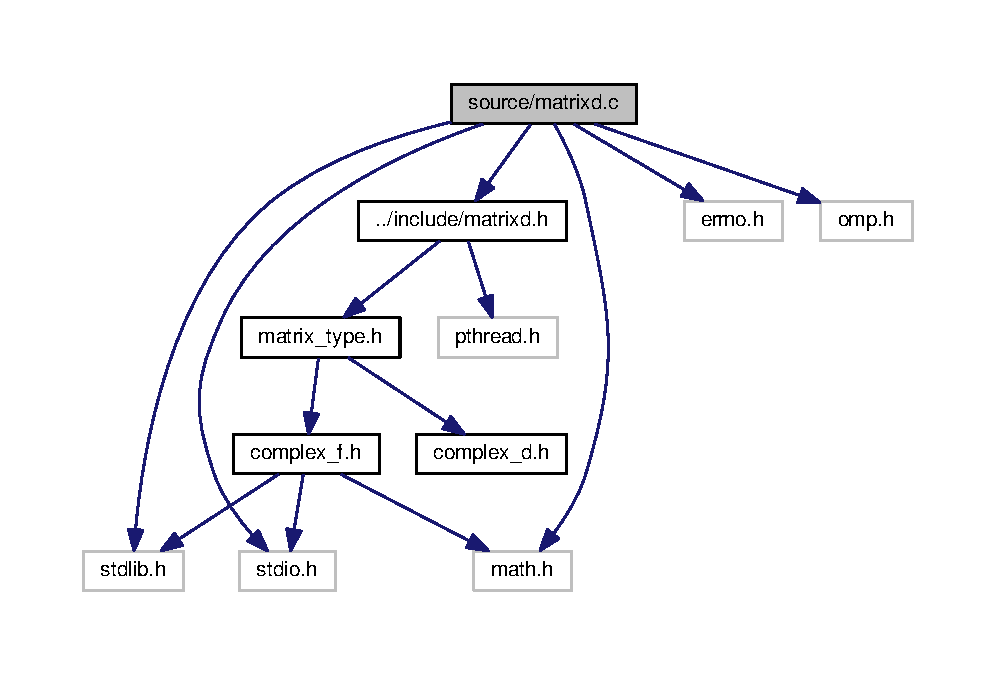
\includegraphics[width=350pt]{matrixd_8c__incl}
\end{center}
\end{figure}
\subsection*{Functions}
\begin{DoxyCompactItemize}
\item 
void \hyperlink{matrixd_8c_aeebf82147e41165a72a1faf5b6f58cbe}{print\+MatrixD} (\hyperlink{structMatrix__d}{Matrix\+\_\+d} $\ast$a)
\begin{DoxyCompactList}\small\item\em print\+MatrixD display a matrix of doubles (usefull for testing) \end{DoxyCompactList}\item 
\hyperlink{structMatrix__d}{Matrix\+\_\+d} $\ast$ \hyperlink{matrixd_8c_a6ff76857b26a8b0fc0eca59bfa849e9a}{matrix\+AllocD} (unsigned int rows, unsigned int column)
\begin{DoxyCompactList}\small\item\em matrix\+AllocD allocate memory for a matrix and initialize it to zero \end{DoxyCompactList}\item 
\hyperlink{structMatrix__d}{Matrix\+\_\+d} $\ast$ \hyperlink{matrixd_8c_ae287aca00d0e858d465407e27505fc86}{create\+Random\+MatrixD} (unsigned int rows, unsigned int column)
\begin{DoxyCompactList}\small\item\em create\+Random\+Matrix initialize a random Matrix \end{DoxyCompactList}\item 
void \hyperlink{matrixd_8c_ac2640483bc926409d0700755b0af5045}{create\+Zero\+MatrixD} (\hyperlink{structMatrix__d}{Matrix\+\_\+d} $\ast$J)
\begin{DoxyCompactList}\small\item\em create\+Random\+Matrix initialize a random Matrix \end{DoxyCompactList}\item 
\hyperlink{structMatrix__d}{Matrix\+\_\+d} $\ast$ \hyperlink{matrixd_8c_adce723f460015224445701f0e393826c}{create\+Test\+VectorD} (unsigned int type)
\begin{DoxyCompactList}\small\item\em create\+Test\+Vector initialize a known vector of size 3\+:1 \end{DoxyCompactList}\item 
void \hyperlink{matrixd_8c_a35dbcfdd7d0125570b4ef3857b351cf2}{create\+IdentityD} (\hyperlink{structMatrix__d}{Matrix\+\_\+d} $\ast$I)
\begin{DoxyCompactList}\small\item\em create\+IdentityD compute the identoty matrix \end{DoxyCompactList}\item 
void \hyperlink{matrixd_8c_aefcf2f0617929d1f004820a0b2ce55fd}{free\+MatrixD} (\hyperlink{structMatrix__d}{Matrix\+\_\+d} $\ast$A)
\begin{DoxyCompactList}\small\item\em free\+MatrixD free a double matrix \end{DoxyCompactList}\item 
double \hyperlink{matrixd_8c_ac3d08df97e27595ae172dbfaa469da95}{matrix\+GetD} (\hyperlink{structMatrix__d}{Matrix\+\_\+d} $\ast$A, unsigned int i, unsigned int j)
\begin{DoxyCompactList}\small\item\em matrix\+GetD access a specified data of a matrix \end{DoxyCompactList}\item 
void \hyperlink{matrixd_8c_a76a5ff922a8c88a4f714c541536174ae}{matrix\+SetD} (\hyperlink{structMatrix__d}{Matrix\+\_\+d} $\ast$A, unsigned int i, unsigned int j, const double c)
\begin{DoxyCompactList}\small\item\em matrix\+SetD set the value of a specified data \end{DoxyCompactList}\item 
void \hyperlink{matrixd_8c_a26a3bae7e0207e93519cacc7f28b9f28}{scale\+MatrixD} (\hyperlink{structMatrix__d}{Matrix\+\_\+d} $\ast$a, const double c)
\begin{DoxyCompactList}\small\item\em scale\+MatrixD multiply each data by a constant () \end{DoxyCompactList}\item 
void \hyperlink{matrixd_8c_ac7de4dcf4c04dd88e30fde5bb6b5fe6f}{add\+MatrixD} (\hyperlink{structMatrix__d}{Matrix\+\_\+d} $\ast$a, \hyperlink{structMatrix__d}{Matrix\+\_\+d} $\ast$b)
\begin{DoxyCompactList}\small\item\em add\+MatrixD compute A = A+B \end{DoxyCompactList}\item 
void \hyperlink{matrixd_8c_a1b8b1198071dba9e22d084a422bc1dff}{add\+Matrix\+TD} (\hyperlink{structMatrix__d}{Matrix\+\_\+d} $\ast$a, \hyperlink{structMatrix__d}{Matrix\+\_\+d} $\ast$b)
\begin{DoxyCompactList}\small\item\em add\+Matrix\+TD compute A = A+\+BT BT being the transposed matrix of B \end{DoxyCompactList}\item 
void \hyperlink{matrixd_8c_a81d4470f1cac6438cb8b2b0efc9bb2b9}{sub\+MatrixD} (\hyperlink{structMatrix__d}{Matrix\+\_\+d} $\ast$a, \hyperlink{structMatrix__d}{Matrix\+\_\+d} $\ast$b)
\begin{DoxyCompactList}\small\item\em sub\+MatrixD compute A = A-\/B \end{DoxyCompactList}\item 
void \hyperlink{matrixd_8c_a69ab2ff6c56dfcda9f40cf34a1703395}{mul\+MatrixD} (\hyperlink{structMatrix__d}{Matrix\+\_\+d} $\ast$a, \hyperlink{structMatrix__d}{Matrix\+\_\+d} $\ast$b, \hyperlink{structMatrix__d}{Matrix\+\_\+d} $\ast$c)
\begin{DoxyCompactList}\small\item\em compute C = A$\ast$B \end{DoxyCompactList}\item 
void \hyperlink{matrixd_8c_af044608679902bc2f10ec41c73d1b9ba}{mat\+RefD} (\hyperlink{structMatrix__d}{Matrix\+\_\+d} $\ast$A)
\begin{DoxyCompactList}\small\item\em mat\+NormD take the first matrix A value as a reference (ie\+: 1) and scale the other value accoarding to that \end{DoxyCompactList}\item 
void \hyperlink{matrixd_8c_ac006431b140f4aa41241b200b1ae2160}{scale\+LineD} (\hyperlink{structMatrix__d}{Matrix\+\_\+d} $\ast$a, unsigned int i, double f)
\begin{DoxyCompactList}\small\item\em scale\+LineD multiply a line with a \end{DoxyCompactList}\item 
int \hyperlink{matrixd_8c_a7d2311a6678cfd6283c9fdbdb14e0c82}{sub\+X\+LinesD} (\hyperlink{structMatrix__d}{Matrix\+\_\+d} $\ast$a, unsigned int i, unsigned int i2, double f)
\begin{DoxyCompactList}\small\item\em sub\+X\+LinesD computes line i -\/ f$\ast$line i2 and store it into line i \end{DoxyCompactList}\item 
void \hyperlink{matrixd_8c_ad7aa0adf79e3a8db63d5bf42fcfb46d9}{mul\+Add\+Scale\+MatrixD} (\hyperlink{structMatrix__d}{Matrix\+\_\+d} $\ast$result, \hyperlink{structMatrix__d}{Matrix\+\_\+d} $\ast$mul1, \hyperlink{structMatrix__d}{Matrix\+\_\+d} $\ast$mul2, \hyperlink{structMatrix__d}{Matrix\+\_\+d} $\ast$add, double l, double s)
\begin{DoxyCompactList}\small\item\em compute result = s$\ast$(mul1$\ast$mul2 + l$\ast$add) \end{DoxyCompactList}\item 
int \hyperlink{matrixd_8c_ad40ecc4702d0b8006c74e5dc9d276bfa}{is\+DiagD} (\hyperlink{structMatrix__d}{Matrix\+\_\+d} $\ast$a)
\begin{DoxyCompactList}\small\item\em checks if the matrix is diagonal and sets its flag if necessary \end{DoxyCompactList}\item 
int \hyperlink{matrixd_8c_a395a85ba238f77a9d99379d7ccb17319}{is\+Tri\+UD} (\hyperlink{structMatrix__d}{Matrix\+\_\+d} $\ast$a)
\begin{DoxyCompactList}\small\item\em checks if the matrix is triangular UP and sets its flag if necessary \end{DoxyCompactList}\item 
int \hyperlink{matrixd_8c_ad2b735851078c82820cbfb6a8bdf50d7}{is\+Tri\+LD} (\hyperlink{structMatrix__d}{Matrix\+\_\+d} $\ast$a)
\begin{DoxyCompactList}\small\item\em checks if the matrix is triangular Low and sets its flag if necessary \end{DoxyCompactList}\item 
int \hyperlink{matrixd_8c_a8f670f030620d51be8576e58eb7c9938}{is\+SparseD} (\hyperlink{structMatrix__d}{Matrix\+\_\+d} $\ast$a)
\begin{DoxyCompactList}\small\item\em checks if the sparcity of the matrix is superior to 2/3 (allows compression) \end{DoxyCompactList}\end{DoxyCompactItemize}


\subsection{Detailed Description}
to handle matrix operations for doubles \begin{DoxyAuthor}{Author}
Nicolas Sourbier 
\end{DoxyAuthor}
\begin{DoxyDate}{Date}
10/09/2018
\end{DoxyDate}
to handle matrix operations for floats \begin{DoxyAuthor}{Author}
Nicolas Sourbier 
\end{DoxyAuthor}
\begin{DoxyDate}{Date}
10/09/2018 
\end{DoxyDate}


\subsection{Function Documentation}
\index{matrixd.\+c@{matrixd.\+c}!add\+MatrixD@{add\+MatrixD}}
\index{add\+MatrixD@{add\+MatrixD}!matrixd.\+c@{matrixd.\+c}}
\subsubsection[{\texorpdfstring{add\+Matrix\+D(\+Matrix\+\_\+d $\ast$a, Matrix\+\_\+d $\ast$b)}{addMatrixD(Matrix_d *a, Matrix_d *b)}}]{\setlength{\rightskip}{0pt plus 5cm}void add\+MatrixD (
\begin{DoxyParamCaption}
\item[{{\bf Matrix\+\_\+d} $\ast$}]{a, }
\item[{{\bf Matrix\+\_\+d} $\ast$}]{b}
\end{DoxyParamCaption}
)}\hypertarget{matrixd_8c_ac7de4dcf4c04dd88e30fde5bb6b5fe6f}{}\label{matrixd_8c_ac7de4dcf4c04dd88e30fde5bb6b5fe6f}


add\+MatrixD compute A = A+B 


\begin{DoxyParams}{Parameters}
{\em a} & matrix \\
\hline
{\em b} & matrix \\
\hline
\end{DoxyParams}
\index{matrixd.\+c@{matrixd.\+c}!add\+Matrix\+TD@{add\+Matrix\+TD}}
\index{add\+Matrix\+TD@{add\+Matrix\+TD}!matrixd.\+c@{matrixd.\+c}}
\subsubsection[{\texorpdfstring{add\+Matrix\+T\+D(\+Matrix\+\_\+d $\ast$a, Matrix\+\_\+d $\ast$b)}{addMatrixTD(Matrix_d *a, Matrix_d *b)}}]{\setlength{\rightskip}{0pt plus 5cm}void add\+Matrix\+TD (
\begin{DoxyParamCaption}
\item[{{\bf Matrix\+\_\+d} $\ast$}]{a, }
\item[{{\bf Matrix\+\_\+d} $\ast$}]{b}
\end{DoxyParamCaption}
)}\hypertarget{matrixd_8c_a1b8b1198071dba9e22d084a422bc1dff}{}\label{matrixd_8c_a1b8b1198071dba9e22d084a422bc1dff}


add\+Matrix\+TD compute A = A+\+BT BT being the transposed matrix of B 


\begin{DoxyParams}{Parameters}
{\em a} & matrix \\
\hline
{\em b} & matrix \\
\hline
\end{DoxyParams}
\index{matrixd.\+c@{matrixd.\+c}!create\+IdentityD@{create\+IdentityD}}
\index{create\+IdentityD@{create\+IdentityD}!matrixd.\+c@{matrixd.\+c}}
\subsubsection[{\texorpdfstring{create\+Identity\+D(\+Matrix\+\_\+d $\ast$\+I)}{createIdentityD(Matrix_d *I)}}]{\setlength{\rightskip}{0pt plus 5cm}void create\+IdentityD (
\begin{DoxyParamCaption}
\item[{{\bf Matrix\+\_\+d} $\ast$}]{id}
\end{DoxyParamCaption}
)}\hypertarget{matrixd_8c_a35dbcfdd7d0125570b4ef3857b351cf2}{}\label{matrixd_8c_a35dbcfdd7d0125570b4ef3857b351cf2}


create\+IdentityD compute the identoty matrix 


\begin{DoxyParams}{Parameters}
{\em id} & A pointer to store the result \\
\hline
\end{DoxyParams}
\index{matrixd.\+c@{matrixd.\+c}!create\+Random\+MatrixD@{create\+Random\+MatrixD}}
\index{create\+Random\+MatrixD@{create\+Random\+MatrixD}!matrixd.\+c@{matrixd.\+c}}
\subsubsection[{\texorpdfstring{create\+Random\+Matrix\+D(unsigned int rows, unsigned int column)}{createRandomMatrixD(unsigned int rows, unsigned int column)}}]{\setlength{\rightskip}{0pt plus 5cm}{\bf Matrix\+\_\+d}$\ast$ create\+Random\+MatrixD (
\begin{DoxyParamCaption}
\item[{unsigned int}]{rows, }
\item[{unsigned int}]{column}
\end{DoxyParamCaption}
)}\hypertarget{matrixd_8c_ae287aca00d0e858d465407e27505fc86}{}\label{matrixd_8c_ae287aca00d0e858d465407e27505fc86}


create\+Random\+Matrix initialize a random Matrix 


\begin{DoxyParams}{Parameters}
{\em rows} & number of rows \\
\hline
{\em column} & number of columns \\
\hline
\end{DoxyParams}
\begin{DoxyReturn}{Returns}
the random matrix 
\end{DoxyReturn}
\index{matrixd.\+c@{matrixd.\+c}!create\+Test\+VectorD@{create\+Test\+VectorD}}
\index{create\+Test\+VectorD@{create\+Test\+VectorD}!matrixd.\+c@{matrixd.\+c}}
\subsubsection[{\texorpdfstring{create\+Test\+Vector\+D(unsigned int type)}{createTestVectorD(unsigned int type)}}]{\setlength{\rightskip}{0pt plus 5cm}{\bf Matrix\+\_\+d}$\ast$ create\+Test\+VectorD (
\begin{DoxyParamCaption}
\item[{unsigned int}]{type}
\end{DoxyParamCaption}
)}\hypertarget{matrixd_8c_adce723f460015224445701f0e393826c}{}\label{matrixd_8c_adce723f460015224445701f0e393826c}


create\+Test\+Vector initialize a known vector of size 3\+:1 


\begin{DoxyParams}{Parameters}
{\em type} & (1 or 2) you can choose between two matrix \\
\hline
\end{DoxyParams}
\begin{DoxyReturn}{Returns}
the random matrix 
\end{DoxyReturn}
\index{matrixd.\+c@{matrixd.\+c}!create\+Zero\+MatrixD@{create\+Zero\+MatrixD}}
\index{create\+Zero\+MatrixD@{create\+Zero\+MatrixD}!matrixd.\+c@{matrixd.\+c}}
\subsubsection[{\texorpdfstring{create\+Zero\+Matrix\+D(\+Matrix\+\_\+d $\ast$\+J)}{createZeroMatrixD(Matrix_d *J)}}]{\setlength{\rightskip}{0pt plus 5cm}void create\+Zero\+MatrixD (
\begin{DoxyParamCaption}
\item[{{\bf Matrix\+\_\+d} $\ast$}]{J}
\end{DoxyParamCaption}
)}\hypertarget{matrixd_8c_ac2640483bc926409d0700755b0af5045}{}\label{matrixd_8c_ac2640483bc926409d0700755b0af5045}


create\+Random\+Matrix initialize a random Matrix 


\begin{DoxyParams}{Parameters}
{\em J} & a matrix to fill with zeros \\
\hline
\end{DoxyParams}
\begin{DoxyReturn}{Returns}
the random matrix 
\end{DoxyReturn}
\index{matrixd.\+c@{matrixd.\+c}!free\+MatrixD@{free\+MatrixD}}
\index{free\+MatrixD@{free\+MatrixD}!matrixd.\+c@{matrixd.\+c}}
\subsubsection[{\texorpdfstring{free\+Matrix\+D(\+Matrix\+\_\+d $\ast$\+A)}{freeMatrixD(Matrix_d *A)}}]{\setlength{\rightskip}{0pt plus 5cm}void free\+MatrixD (
\begin{DoxyParamCaption}
\item[{{\bf Matrix\+\_\+d} $\ast$}]{A}
\end{DoxyParamCaption}
)}\hypertarget{matrixd_8c_aefcf2f0617929d1f004820a0b2ce55fd}{}\label{matrixd_8c_aefcf2f0617929d1f004820a0b2ce55fd}


free\+MatrixD free a double matrix 


\begin{DoxyParams}{Parameters}
{\em A} & the matrix to free \\
\hline
\end{DoxyParams}
\index{matrixd.\+c@{matrixd.\+c}!is\+DiagD@{is\+DiagD}}
\index{is\+DiagD@{is\+DiagD}!matrixd.\+c@{matrixd.\+c}}
\subsubsection[{\texorpdfstring{is\+Diag\+D(\+Matrix\+\_\+d $\ast$a)}{isDiagD(Matrix_d *a)}}]{\setlength{\rightskip}{0pt plus 5cm}int is\+DiagD (
\begin{DoxyParamCaption}
\item[{{\bf Matrix\+\_\+d} $\ast$}]{a}
\end{DoxyParamCaption}
)}\hypertarget{matrixd_8c_ad40ecc4702d0b8006c74e5dc9d276bfa}{}\label{matrixd_8c_ad40ecc4702d0b8006c74e5dc9d276bfa}


checks if the matrix is diagonal and sets its flag if necessary 


\begin{DoxyParams}{Parameters}
{\em a} & the matrix to test returns 1 if diag, 0 otherwise \\
\hline
\end{DoxyParams}
\index{matrixd.\+c@{matrixd.\+c}!is\+SparseD@{is\+SparseD}}
\index{is\+SparseD@{is\+SparseD}!matrixd.\+c@{matrixd.\+c}}
\subsubsection[{\texorpdfstring{is\+Sparse\+D(\+Matrix\+\_\+d $\ast$a)}{isSparseD(Matrix_d *a)}}]{\setlength{\rightskip}{0pt plus 5cm}int is\+SparseD (
\begin{DoxyParamCaption}
\item[{{\bf Matrix\+\_\+d} $\ast$}]{a}
\end{DoxyParamCaption}
)}\hypertarget{matrixd_8c_a8f670f030620d51be8576e58eb7c9938}{}\label{matrixd_8c_a8f670f030620d51be8576e58eb7c9938}


checks if the sparcity of the matrix is superior to 2/3 (allows compression) 


\begin{DoxyParams}{Parameters}
{\em a} & the matrix to test returns 1 if diag, 0 otherwise \\
\hline
\end{DoxyParams}
\index{matrixd.\+c@{matrixd.\+c}!is\+Tri\+LD@{is\+Tri\+LD}}
\index{is\+Tri\+LD@{is\+Tri\+LD}!matrixd.\+c@{matrixd.\+c}}
\subsubsection[{\texorpdfstring{is\+Tri\+L\+D(\+Matrix\+\_\+d $\ast$a)}{isTriLD(Matrix_d *a)}}]{\setlength{\rightskip}{0pt plus 5cm}int is\+Tri\+LD (
\begin{DoxyParamCaption}
\item[{{\bf Matrix\+\_\+d} $\ast$}]{a}
\end{DoxyParamCaption}
)}\hypertarget{matrixd_8c_ad2b735851078c82820cbfb6a8bdf50d7}{}\label{matrixd_8c_ad2b735851078c82820cbfb6a8bdf50d7}


checks if the matrix is triangular Low and sets its flag if necessary 


\begin{DoxyParams}{Parameters}
{\em a} & the matrix to test returns 1 if diag, 0 otherwise \\
\hline
\end{DoxyParams}
\index{matrixd.\+c@{matrixd.\+c}!is\+Tri\+UD@{is\+Tri\+UD}}
\index{is\+Tri\+UD@{is\+Tri\+UD}!matrixd.\+c@{matrixd.\+c}}
\subsubsection[{\texorpdfstring{is\+Tri\+U\+D(\+Matrix\+\_\+d $\ast$a)}{isTriUD(Matrix_d *a)}}]{\setlength{\rightskip}{0pt plus 5cm}int is\+Tri\+UD (
\begin{DoxyParamCaption}
\item[{{\bf Matrix\+\_\+d} $\ast$}]{a}
\end{DoxyParamCaption}
)}\hypertarget{matrixd_8c_a395a85ba238f77a9d99379d7ccb17319}{}\label{matrixd_8c_a395a85ba238f77a9d99379d7ccb17319}


checks if the matrix is triangular UP and sets its flag if necessary 


\begin{DoxyParams}{Parameters}
{\em a} & the matrix to test returns 1 if diag, 0 otherwise \\
\hline
\end{DoxyParams}
\index{matrixd.\+c@{matrixd.\+c}!mat\+RefD@{mat\+RefD}}
\index{mat\+RefD@{mat\+RefD}!matrixd.\+c@{matrixd.\+c}}
\subsubsection[{\texorpdfstring{mat\+Ref\+D(\+Matrix\+\_\+d $\ast$\+A)}{matRefD(Matrix_d *A)}}]{\setlength{\rightskip}{0pt plus 5cm}void mat\+RefD (
\begin{DoxyParamCaption}
\item[{{\bf Matrix\+\_\+d} $\ast$}]{A}
\end{DoxyParamCaption}
)}\hypertarget{matrixd_8c_af044608679902bc2f10ec41c73d1b9ba}{}\label{matrixd_8c_af044608679902bc2f10ec41c73d1b9ba}


mat\+NormD take the first matrix A value as a reference (ie\+: 1) and scale the other value accoarding to that 


\begin{DoxyParams}{Parameters}
{\em A} & the matrix that we want to \char`\"{}norm\char`\"{} \\
\hline
\end{DoxyParams}
\index{matrixd.\+c@{matrixd.\+c}!matrix\+AllocD@{matrix\+AllocD}}
\index{matrix\+AllocD@{matrix\+AllocD}!matrixd.\+c@{matrixd.\+c}}
\subsubsection[{\texorpdfstring{matrix\+Alloc\+D(unsigned int rows, unsigned int column)}{matrixAllocD(unsigned int rows, unsigned int column)}}]{\setlength{\rightskip}{0pt plus 5cm}{\bf Matrix\+\_\+d}$\ast$ matrix\+AllocD (
\begin{DoxyParamCaption}
\item[{unsigned int}]{rows, }
\item[{unsigned int}]{column}
\end{DoxyParamCaption}
)}\hypertarget{matrixd_8c_a6ff76857b26a8b0fc0eca59bfa849e9a}{}\label{matrixd_8c_a6ff76857b26a8b0fc0eca59bfa849e9a}


matrix\+AllocD allocate memory for a matrix and initialize it to zero 


\begin{DoxyParams}{Parameters}
{\em rows} & number of rows \\
\hline
{\em column} & number of columns \\
\hline
\end{DoxyParams}
\begin{DoxyReturn}{Returns}
the allocated matrix if no errors occured, N\+U\+LL if not 
\end{DoxyReturn}
\index{matrixd.\+c@{matrixd.\+c}!matrix\+GetD@{matrix\+GetD}}
\index{matrix\+GetD@{matrix\+GetD}!matrixd.\+c@{matrixd.\+c}}
\subsubsection[{\texorpdfstring{matrix\+Get\+D(\+Matrix\+\_\+d $\ast$\+A, unsigned int i, unsigned int j)}{matrixGetD(Matrix_d *A, unsigned int i, unsigned int j)}}]{\setlength{\rightskip}{0pt plus 5cm}double matrix\+GetD (
\begin{DoxyParamCaption}
\item[{{\bf Matrix\+\_\+d} $\ast$}]{A, }
\item[{unsigned int}]{i, }
\item[{unsigned int}]{j}
\end{DoxyParamCaption}
)}\hypertarget{matrixd_8c_ac3d08df97e27595ae172dbfaa469da95}{}\label{matrixd_8c_ac3d08df97e27595ae172dbfaa469da95}


matrix\+GetD access a specified data of a matrix 


\begin{DoxyParams}{Parameters}
{\em A} & the matrix \\
\hline
{\em i} & the index of rows \\
\hline
{\em j} & the index on columns \\
\hline
\end{DoxyParams}
\begin{DoxyReturn}{Returns}
the data A(i,j) 
\end{DoxyReturn}
\begin{DoxyWarning}{Warning}
if the matrix in parameter is N\+U\+LL, returns 0 
\end{DoxyWarning}
\index{matrixd.\+c@{matrixd.\+c}!matrix\+SetD@{matrix\+SetD}}
\index{matrix\+SetD@{matrix\+SetD}!matrixd.\+c@{matrixd.\+c}}
\subsubsection[{\texorpdfstring{matrix\+Set\+D(\+Matrix\+\_\+d $\ast$\+A, unsigned int i, unsigned int j, const double c)}{matrixSetD(Matrix_d *A, unsigned int i, unsigned int j, const double c)}}]{\setlength{\rightskip}{0pt plus 5cm}void matrix\+SetD (
\begin{DoxyParamCaption}
\item[{{\bf Matrix\+\_\+d} $\ast$}]{A, }
\item[{unsigned int}]{i, }
\item[{unsigned int}]{j, }
\item[{const double}]{c}
\end{DoxyParamCaption}
)}\hypertarget{matrixd_8c_a76a5ff922a8c88a4f714c541536174ae}{}\label{matrixd_8c_a76a5ff922a8c88a4f714c541536174ae}


matrix\+SetD set the value of a specified data 


\begin{DoxyParams}{Parameters}
{\em A} & the matrix \\
\hline
{\em i} & the index on rows \\
\hline
{\em j} & the index on columns \\
\hline
{\em c} & the to set at A(i,j) \\
\hline
\end{DoxyParams}
\index{matrixd.\+c@{matrixd.\+c}!mul\+Add\+Scale\+MatrixD@{mul\+Add\+Scale\+MatrixD}}
\index{mul\+Add\+Scale\+MatrixD@{mul\+Add\+Scale\+MatrixD}!matrixd.\+c@{matrixd.\+c}}
\subsubsection[{\texorpdfstring{mul\+Add\+Scale\+Matrix\+D(\+Matrix\+\_\+d $\ast$result, Matrix\+\_\+d $\ast$mul1, Matrix\+\_\+d $\ast$mul2, Matrix\+\_\+d $\ast$add, double l, double s)}{mulAddScaleMatrixD(Matrix_d *result, Matrix_d *mul1, Matrix_d *mul2, Matrix_d *add, double l, double s)}}]{\setlength{\rightskip}{0pt plus 5cm}void mul\+Add\+Scale\+MatrixD (
\begin{DoxyParamCaption}
\item[{{\bf Matrix\+\_\+d} $\ast$}]{result, }
\item[{{\bf Matrix\+\_\+d} $\ast$}]{mul1, }
\item[{{\bf Matrix\+\_\+d} $\ast$}]{mul2, }
\item[{{\bf Matrix\+\_\+d} $\ast$}]{add, }
\item[{double}]{l, }
\item[{double}]{s}
\end{DoxyParamCaption}
)}\hypertarget{matrixd_8c_ad7aa0adf79e3a8db63d5bf42fcfb46d9}{}\label{matrixd_8c_ad7aa0adf79e3a8db63d5bf42fcfb46d9}


compute result = s$\ast$(mul1$\ast$mul2 + l$\ast$add) 


\begin{DoxyParams}{Parameters}
{\em result} & a matrix to store the result \\
\hline
{\em mul1} & \& \\
\hline
{\em mul2} & matrices to multiply \\
\hline
{\em add} & a matrix to add to the previous product \\
\hline
{\em l} & a double to scale the add matrix \\
\hline
{\em s} & a double to scale the result doesn\textquotesingle{}t use optimisations related to the matrix properties \\
\hline
\end{DoxyParams}
\index{matrixd.\+c@{matrixd.\+c}!mul\+MatrixD@{mul\+MatrixD}}
\index{mul\+MatrixD@{mul\+MatrixD}!matrixd.\+c@{matrixd.\+c}}
\subsubsection[{\texorpdfstring{mul\+Matrix\+D(\+Matrix\+\_\+d $\ast$a, Matrix\+\_\+d $\ast$b, Matrix\+\_\+d $\ast$c)}{mulMatrixD(Matrix_d *a, Matrix_d *b, Matrix_d *c)}}]{\setlength{\rightskip}{0pt plus 5cm}void mul\+MatrixD (
\begin{DoxyParamCaption}
\item[{{\bf Matrix\+\_\+d} $\ast$}]{a, }
\item[{{\bf Matrix\+\_\+d} $\ast$}]{b, }
\item[{{\bf Matrix\+\_\+d} $\ast$}]{c}
\end{DoxyParamCaption}
)}\hypertarget{matrixd_8c_a69ab2ff6c56dfcda9f40cf34a1703395}{}\label{matrixd_8c_a69ab2ff6c56dfcda9f40cf34a1703395}


compute C = A$\ast$B 


\begin{DoxyParams}{Parameters}
{\em a} & matrix \\
\hline
{\em b} & matrix \\
\hline
{\em c} & a matrix to store the result \\
\hline
\end{DoxyParams}
\index{matrixd.\+c@{matrixd.\+c}!print\+MatrixD@{print\+MatrixD}}
\index{print\+MatrixD@{print\+MatrixD}!matrixd.\+c@{matrixd.\+c}}
\subsubsection[{\texorpdfstring{print\+Matrix\+D(\+Matrix\+\_\+d $\ast$a)}{printMatrixD(Matrix_d *a)}}]{\setlength{\rightskip}{0pt plus 5cm}void print\+MatrixD (
\begin{DoxyParamCaption}
\item[{{\bf Matrix\+\_\+d} $\ast$}]{a}
\end{DoxyParamCaption}
)}\hypertarget{matrixd_8c_aeebf82147e41165a72a1faf5b6f58cbe}{}\label{matrixd_8c_aeebf82147e41165a72a1faf5b6f58cbe}


print\+MatrixD display a matrix of doubles (usefull for testing) 


\begin{DoxyParams}{Parameters}
{\em a} & the matrix to display \\
\hline
\end{DoxyParams}
\index{matrixd.\+c@{matrixd.\+c}!scale\+LineD@{scale\+LineD}}
\index{scale\+LineD@{scale\+LineD}!matrixd.\+c@{matrixd.\+c}}
\subsubsection[{\texorpdfstring{scale\+Line\+D(\+Matrix\+\_\+d $\ast$a, unsigned int i, double f)}{scaleLineD(Matrix_d *a, unsigned int i, double f)}}]{\setlength{\rightskip}{0pt plus 5cm}void scale\+LineD (
\begin{DoxyParamCaption}
\item[{{\bf Matrix\+\_\+d} $\ast$}]{a, }
\item[{unsigned int}]{i, }
\item[{double}]{f}
\end{DoxyParamCaption}
)}\hypertarget{matrixd_8c_ac006431b140f4aa41241b200b1ae2160}{}\label{matrixd_8c_ac006431b140f4aa41241b200b1ae2160}


scale\+LineD multiply a line with a 


\begin{DoxyParams}{Parameters}
{\em a} & the matrix \\
\hline
{\em i} & the index of the line we want to scale \\
\hline
{\em f} & the that will scale the line \\
\hline
\end{DoxyParams}
\index{matrixd.\+c@{matrixd.\+c}!scale\+MatrixD@{scale\+MatrixD}}
\index{scale\+MatrixD@{scale\+MatrixD}!matrixd.\+c@{matrixd.\+c}}
\subsubsection[{\texorpdfstring{scale\+Matrix\+D(\+Matrix\+\_\+d $\ast$a, const double c)}{scaleMatrixD(Matrix_d *a, const double c)}}]{\setlength{\rightskip}{0pt plus 5cm}void scale\+MatrixD (
\begin{DoxyParamCaption}
\item[{{\bf Matrix\+\_\+d} $\ast$}]{a, }
\item[{const double}]{c}
\end{DoxyParamCaption}
)}\hypertarget{matrixd_8c_a26a3bae7e0207e93519cacc7f28b9f28}{}\label{matrixd_8c_a26a3bae7e0207e93519cacc7f28b9f28}


scale\+MatrixD multiply each data by a constant () 


\begin{DoxyParams}{Parameters}
{\em a} & the matrix to scale \\
\hline
{\em c} & the \\
\hline
\end{DoxyParams}
\index{matrixd.\+c@{matrixd.\+c}!sub\+MatrixD@{sub\+MatrixD}}
\index{sub\+MatrixD@{sub\+MatrixD}!matrixd.\+c@{matrixd.\+c}}
\subsubsection[{\texorpdfstring{sub\+Matrix\+D(\+Matrix\+\_\+d $\ast$a, Matrix\+\_\+d $\ast$b)}{subMatrixD(Matrix_d *a, Matrix_d *b)}}]{\setlength{\rightskip}{0pt plus 5cm}void sub\+MatrixD (
\begin{DoxyParamCaption}
\item[{{\bf Matrix\+\_\+d} $\ast$}]{a, }
\item[{{\bf Matrix\+\_\+d} $\ast$}]{b}
\end{DoxyParamCaption}
)}\hypertarget{matrixd_8c_a81d4470f1cac6438cb8b2b0efc9bb2b9}{}\label{matrixd_8c_a81d4470f1cac6438cb8b2b0efc9bb2b9}


sub\+MatrixD compute A = A-\/B 


\begin{DoxyParams}{Parameters}
{\em a} & matrix \\
\hline
{\em b} & matrix \\
\hline
\end{DoxyParams}
\index{matrixd.\+c@{matrixd.\+c}!sub\+X\+LinesD@{sub\+X\+LinesD}}
\index{sub\+X\+LinesD@{sub\+X\+LinesD}!matrixd.\+c@{matrixd.\+c}}
\subsubsection[{\texorpdfstring{sub\+X\+Lines\+D(\+Matrix\+\_\+d $\ast$a, unsigned int i, unsigned int i2, double f)}{subXLinesD(Matrix_d *a, unsigned int i, unsigned int i2, double f)}}]{\setlength{\rightskip}{0pt plus 5cm}int sub\+X\+LinesD (
\begin{DoxyParamCaption}
\item[{{\bf Matrix\+\_\+d} $\ast$}]{a, }
\item[{unsigned int}]{i, }
\item[{unsigned int}]{i2, }
\item[{double}]{f}
\end{DoxyParamCaption}
)}\hypertarget{matrixd_8c_a7d2311a6678cfd6283c9fdbdb14e0c82}{}\label{matrixd_8c_a7d2311a6678cfd6283c9fdbdb14e0c82}


sub\+X\+LinesD computes line i -\/ f$\ast$line i2 and store it into line i 


\begin{DoxyParams}{Parameters}
{\em a} & the matrix \\
\hline
{\em i} & the index of the line to update \\
\hline
{\em i2} & the index of the \char`\"{}reference\char`\"{} line \\
\hline
{\em f} & a to scale the matrix \\
\hline
\end{DoxyParams}

\hypertarget{matrixf_8c}{}\section{source/matrixf.c File Reference}
\label{matrixf_8c}\index{source/matrixf.\+c@{source/matrixf.\+c}}
{\ttfamily \#include $<$stdlib.\+h$>$}\\*
{\ttfamily \#include $<$stdio.\+h$>$}\\*
{\ttfamily \#include $<$math.\+h$>$}\\*
{\ttfamily \#include \char`\"{}../include/matrixf.\+h\char`\"{}}\\*
{\ttfamily \#include \char`\"{}errno.\+h\char`\"{}}\\*
{\ttfamily \#include $<$omp.\+h$>$}\\*
Include dependency graph for matrixf.\+c\+:
\nopagebreak
\begin{figure}[H]
\begin{center}
\leavevmode
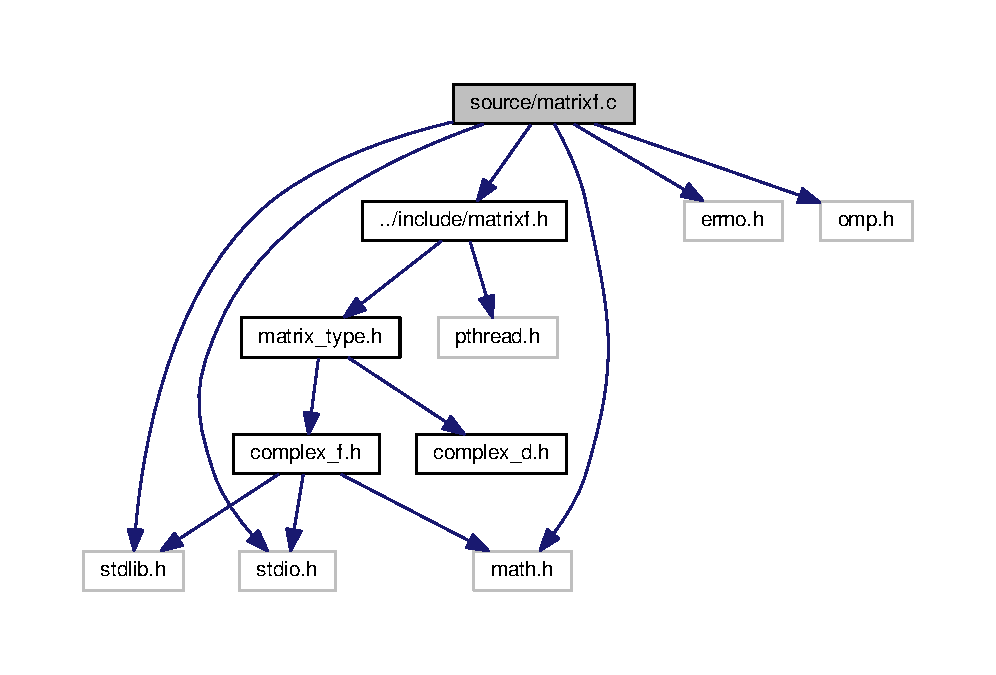
\includegraphics[width=350pt]{matrixf_8c__incl}
\end{center}
\end{figure}
\subsection*{Functions}
\begin{DoxyCompactItemize}
\item 
\hyperlink{structMatrix__f}{Matrix\+\_\+f} $\ast$ \hyperlink{matrixf_8c_a0765510a29128648da66826dea1f7c4f}{read\+Matrix\+\_\+f\+\_\+\+File} (char $\ast$filename)
\begin{DoxyCompactList}\small\item\em reads a matrix from a binary file \end{DoxyCompactList}\item 
int \hyperlink{matrixf_8c_ad4b504bfe17f177776b461ef1c789c23}{write\+Matrix\+\_\+f\+\_\+\+File} (char $\ast$filename, \hyperlink{structMatrix__f}{Matrix\+\_\+f} $\ast$ptr)
\begin{DoxyCompactList}\small\item\em writes a matrix in a binary file \end{DoxyCompactList}\item 
void \hyperlink{matrixf_8c_a65db426ed594e233c1cf08b1d764959c}{print\+MatrixF} (\hyperlink{structMatrix__f}{Matrix\+\_\+f} $\ast$a)
\begin{DoxyCompactList}\small\item\em print\+MatrixF display a matrix of floats (usefull for testing) \end{DoxyCompactList}\item 
\hyperlink{structMatrix__f}{Matrix\+\_\+f} $\ast$ \hyperlink{matrixf_8c_a1f51ad263d26309b1bafb936711b16a4}{matrix\+AllocF} (unsigned int rows, unsigned int column)
\begin{DoxyCompactList}\small\item\em matrix\+AllocF allocate memory for a matrix and initialize it to zero \end{DoxyCompactList}\item 
\hyperlink{structMatrix__f}{Matrix\+\_\+f} $\ast$ \hyperlink{matrixf_8c_a01f8ab8924800d7a7b3b5ba4c05a3df7}{create\+Random\+MatrixF} (unsigned int rows, unsigned int column)
\begin{DoxyCompactList}\small\item\em create\+Random\+Matrix initialize a random Matrix \end{DoxyCompactList}\item 
void \hyperlink{matrixf_8c_a36a5e23d99c41a4d90fadfefde1e8d89}{create\+Zero\+MatrixF} (\hyperlink{structMatrix__f}{Matrix\+\_\+f} $\ast$J)
\begin{DoxyCompactList}\small\item\em create\+Random\+Matrix initialize a random Matrix \end{DoxyCompactList}\item 
\hyperlink{structMatrix__f}{Matrix\+\_\+f} $\ast$ \hyperlink{matrixf_8c_a6f921af99507db80e4f0edd83b6b9d74}{create\+Test\+VectorF} (unsigned int type)
\begin{DoxyCompactList}\small\item\em create\+Test\+Vector initialize a known vector of size 3\+:1 \end{DoxyCompactList}\item 
void \hyperlink{matrixf_8c_ae21e92877568f8f9d467f4e8ed7b2287}{create\+IdentityF} (\hyperlink{structMatrix__f}{Matrix\+\_\+f} $\ast$I)
\begin{DoxyCompactList}\small\item\em create\+IdentityF compute the identoty matrix \end{DoxyCompactList}\item 
void \hyperlink{matrixf_8c_a3fce8551cf9e3287f1ce6f69441d08de}{free\+MatrixF} (\hyperlink{structMatrix__f}{Matrix\+\_\+f} $\ast$A)
\begin{DoxyCompactList}\small\item\em free\+MatrixF free a float matrix \end{DoxyCompactList}\item 
float \hyperlink{matrixf_8c_abbbe59dd5fda26fb31b2d151f503f070}{matrix\+GetF} (\hyperlink{structMatrix__f}{Matrix\+\_\+f} $\ast$A, unsigned int i, unsigned int j)
\begin{DoxyCompactList}\small\item\em matrix\+GetF access a specified data of a matrix \end{DoxyCompactList}\item 
void \hyperlink{matrixf_8c_a7de342d52dcab8d64a65979ebf5796a3}{matrix\+SetF} (\hyperlink{structMatrix__f}{Matrix\+\_\+f} $\ast$A, unsigned int i, unsigned int j, const float c)
\begin{DoxyCompactList}\small\item\em matrix\+SetF set the value of a specified data \end{DoxyCompactList}\item 
void \hyperlink{matrixf_8c_a21f7154c7ca6e677418970cc0f7580b2}{scale\+MatrixF} (\hyperlink{structMatrix__f}{Matrix\+\_\+f} $\ast$a, const float c)
\begin{DoxyCompactList}\small\item\em scale\+MatrixF multiply each data by a constant () \end{DoxyCompactList}\item 
void \hyperlink{matrixf_8c_a3429b21ef1a46341663ce8e3671c6d10}{add\+MatrixF} (\hyperlink{structMatrix__f}{Matrix\+\_\+f} $\ast$a, \hyperlink{structMatrix__f}{Matrix\+\_\+f} $\ast$b)
\begin{DoxyCompactList}\small\item\em add\+MatrixF compute A = A+B \end{DoxyCompactList}\item 
void \hyperlink{matrixf_8c_a41b29f1f48abd5b646772a036d89c8ca}{add\+Matrix\+TF} (\hyperlink{structMatrix__f}{Matrix\+\_\+f} $\ast$a, \hyperlink{structMatrix__f}{Matrix\+\_\+f} $\ast$b)
\begin{DoxyCompactList}\small\item\em add\+Matrix\+TF compute A = A+\+BT BT being the transposed matrix of B \end{DoxyCompactList}\item 
void \hyperlink{matrixf_8c_aaaa2090c3e8c3f482be2d41c219528ed}{sub\+MatrixF} (\hyperlink{structMatrix__f}{Matrix\+\_\+f} $\ast$a, \hyperlink{structMatrix__f}{Matrix\+\_\+f} $\ast$b)
\begin{DoxyCompactList}\small\item\em sub\+MatrixF compute A = A-\/B \end{DoxyCompactList}\item 
void \hyperlink{matrixf_8c_a813950c5218dab2898ef1a5bea4aaa9f}{scale\+Sub\+MatrixF} (\hyperlink{structMatrix__f}{Matrix\+\_\+f} $\ast$res, \hyperlink{structMatrix__f}{Matrix\+\_\+f} $\ast$mask, float l)
\begin{DoxyCompactList}\small\item\em sub\+MatrixF compute res = res -\/ l$\ast$mask used for deconvolution \end{DoxyCompactList}\item 
void \hyperlink{matrixf_8c_a2da9c79ac2fc5df2801284c79c379b36}{mul\+MatrixF} (\hyperlink{structMatrix__f}{Matrix\+\_\+f} $\ast$a, \hyperlink{structMatrix__f}{Matrix\+\_\+f} $\ast$b, \hyperlink{structMatrix__f}{Matrix\+\_\+f} $\ast$c)
\begin{DoxyCompactList}\small\item\em compute C = A$\ast$B \end{DoxyCompactList}\item 
void \hyperlink{matrixf_8c_a64c4c676a46aebc9298c55e66ea90b7c}{mat\+RefF} (\hyperlink{structMatrix__f}{Matrix\+\_\+f} $\ast$A)
\begin{DoxyCompactList}\small\item\em mat\+NormF take the first matrix A value as a reference (ie\+: 1) and scale the other value accoarding to that \end{DoxyCompactList}\item 
void \hyperlink{matrixf_8c_a0c492863193fa933287a4a688facadac}{scale\+LineF} (\hyperlink{structMatrix__f}{Matrix\+\_\+f} $\ast$a, unsigned int i, float f)
\begin{DoxyCompactList}\small\item\em scale\+LineF multiply a line with a \end{DoxyCompactList}\item 
int \hyperlink{matrixf_8c_af9c347f3eaea5e436daf1b6e6b7adbf9}{sub\+X\+LinesF} (\hyperlink{structMatrix__f}{Matrix\+\_\+f} $\ast$a, unsigned int i, unsigned int i2, float f)
\begin{DoxyCompactList}\small\item\em sub\+X\+LinesF computes line i -\/ f$\ast$line i2 and store it into line i \end{DoxyCompactList}\item 
void \hyperlink{matrixf_8c_a889a050642d4698c0ab4a31a2158280c}{mul\+Add\+Scale\+MatrixF} (\hyperlink{structMatrix__f}{Matrix\+\_\+f} $\ast$result, \hyperlink{structMatrix__f}{Matrix\+\_\+f} $\ast$mul1, \hyperlink{structMatrix__f}{Matrix\+\_\+f} $\ast$mul2, \hyperlink{structMatrix__f}{Matrix\+\_\+f} $\ast$add, float l, float s)
\begin{DoxyCompactList}\small\item\em compute result = s$\ast$(mul1$\ast$mul2 + l$\ast$add) \end{DoxyCompactList}\item 
int \hyperlink{matrixf_8c_a4cc1d6b5f0241941680182bbaa7edef0}{is\+DiagF} (\hyperlink{structMatrix__f}{Matrix\+\_\+f} $\ast$a)
\begin{DoxyCompactList}\small\item\em checks if the matrix is diagonal and sets its flag if necessary \end{DoxyCompactList}\item 
int \hyperlink{matrixf_8c_a3ab008736bb3775cc8fee85a8f7376af}{is\+Tri\+UF} (\hyperlink{structMatrix__f}{Matrix\+\_\+f} $\ast$a)
\begin{DoxyCompactList}\small\item\em checks if the matrix is triangular UP and sets its flag if necessary \end{DoxyCompactList}\item 
int \hyperlink{matrixf_8c_a952b658f317dbb9122051bb2df0c749a}{is\+Tri\+LF} (\hyperlink{structMatrix__f}{Matrix\+\_\+f} $\ast$a)
\begin{DoxyCompactList}\small\item\em checks if the matrix is triangular Low and sets its flag if necessary \end{DoxyCompactList}\item 
int \hyperlink{matrixf_8c_a9369107ea221c2347b0e3d039b20d18c}{is\+SparseF} (\hyperlink{structMatrix__f}{Matrix\+\_\+f} $\ast$a)
\begin{DoxyCompactList}\small\item\em checks if the sparcity of the matrix is superior to 2/3 (allows compression) \end{DoxyCompactList}\end{DoxyCompactItemize}


\subsection{Detailed Description}
to handle matrix operations for floats \begin{DoxyAuthor}{Author}
Nicolas Sourbier 
\end{DoxyAuthor}
\begin{DoxyDate}{Date}
10/09/2018 
\end{DoxyDate}


\subsection{Function Documentation}
\index{matrixf.\+c@{matrixf.\+c}!add\+MatrixF@{add\+MatrixF}}
\index{add\+MatrixF@{add\+MatrixF}!matrixf.\+c@{matrixf.\+c}}
\subsubsection[{\texorpdfstring{add\+Matrix\+F(\+Matrix\+\_\+f $\ast$a, Matrix\+\_\+f $\ast$b)}{addMatrixF(Matrix_f *a, Matrix_f *b)}}]{\setlength{\rightskip}{0pt plus 5cm}void add\+MatrixF (
\begin{DoxyParamCaption}
\item[{{\bf Matrix\+\_\+f} $\ast$}]{a, }
\item[{{\bf Matrix\+\_\+f} $\ast$}]{b}
\end{DoxyParamCaption}
)}\hypertarget{matrixf_8c_a3429b21ef1a46341663ce8e3671c6d10}{}\label{matrixf_8c_a3429b21ef1a46341663ce8e3671c6d10}


add\+MatrixF compute A = A+B 


\begin{DoxyParams}{Parameters}
{\em a} & matrix \\
\hline
{\em b} & matrix \\
\hline
\end{DoxyParams}
\index{matrixf.\+c@{matrixf.\+c}!add\+Matrix\+TF@{add\+Matrix\+TF}}
\index{add\+Matrix\+TF@{add\+Matrix\+TF}!matrixf.\+c@{matrixf.\+c}}
\subsubsection[{\texorpdfstring{add\+Matrix\+T\+F(\+Matrix\+\_\+f $\ast$a, Matrix\+\_\+f $\ast$b)}{addMatrixTF(Matrix_f *a, Matrix_f *b)}}]{\setlength{\rightskip}{0pt plus 5cm}void add\+Matrix\+TF (
\begin{DoxyParamCaption}
\item[{{\bf Matrix\+\_\+f} $\ast$}]{a, }
\item[{{\bf Matrix\+\_\+f} $\ast$}]{b}
\end{DoxyParamCaption}
)}\hypertarget{matrixf_8c_a41b29f1f48abd5b646772a036d89c8ca}{}\label{matrixf_8c_a41b29f1f48abd5b646772a036d89c8ca}


add\+Matrix\+TF compute A = A+\+BT BT being the transposed matrix of B 


\begin{DoxyParams}{Parameters}
{\em a} & matrix \\
\hline
{\em b} & matrix \\
\hline
\end{DoxyParams}
\index{matrixf.\+c@{matrixf.\+c}!create\+IdentityF@{create\+IdentityF}}
\index{create\+IdentityF@{create\+IdentityF}!matrixf.\+c@{matrixf.\+c}}
\subsubsection[{\texorpdfstring{create\+Identity\+F(\+Matrix\+\_\+f $\ast$\+I)}{createIdentityF(Matrix_f *I)}}]{\setlength{\rightskip}{0pt plus 5cm}void create\+IdentityF (
\begin{DoxyParamCaption}
\item[{{\bf Matrix\+\_\+f} $\ast$}]{}
\end{DoxyParamCaption}
)}\hypertarget{matrixf_8c_ae21e92877568f8f9d467f4e8ed7b2287}{}\label{matrixf_8c_ae21e92877568f8f9d467f4e8ed7b2287}


create\+IdentityF compute the identoty matrix 


\begin{DoxyParams}{Parameters}
{\em I} & A pointer to store the result \\
\hline
\end{DoxyParams}
\index{matrixf.\+c@{matrixf.\+c}!create\+Random\+MatrixF@{create\+Random\+MatrixF}}
\index{create\+Random\+MatrixF@{create\+Random\+MatrixF}!matrixf.\+c@{matrixf.\+c}}
\subsubsection[{\texorpdfstring{create\+Random\+Matrix\+F(unsigned int rows, unsigned int column)}{createRandomMatrixF(unsigned int rows, unsigned int column)}}]{\setlength{\rightskip}{0pt plus 5cm}{\bf Matrix\+\_\+f}$\ast$ create\+Random\+MatrixF (
\begin{DoxyParamCaption}
\item[{unsigned int}]{rows, }
\item[{unsigned int}]{column}
\end{DoxyParamCaption}
)}\hypertarget{matrixf_8c_a01f8ab8924800d7a7b3b5ba4c05a3df7}{}\label{matrixf_8c_a01f8ab8924800d7a7b3b5ba4c05a3df7}


create\+Random\+Matrix initialize a random Matrix 


\begin{DoxyParams}{Parameters}
{\em rows} & number of rows \\
\hline
{\em column} & number of columns \\
\hline
\end{DoxyParams}
\begin{DoxyReturn}{Returns}
the random matrix 
\end{DoxyReturn}
\index{matrixf.\+c@{matrixf.\+c}!create\+Test\+VectorF@{create\+Test\+VectorF}}
\index{create\+Test\+VectorF@{create\+Test\+VectorF}!matrixf.\+c@{matrixf.\+c}}
\subsubsection[{\texorpdfstring{create\+Test\+Vector\+F(unsigned int type)}{createTestVectorF(unsigned int type)}}]{\setlength{\rightskip}{0pt plus 5cm}{\bf Matrix\+\_\+f}$\ast$ create\+Test\+VectorF (
\begin{DoxyParamCaption}
\item[{unsigned int}]{type}
\end{DoxyParamCaption}
)}\hypertarget{matrixf_8c_a6f921af99507db80e4f0edd83b6b9d74}{}\label{matrixf_8c_a6f921af99507db80e4f0edd83b6b9d74}


create\+Test\+Vector initialize a known vector of size 3\+:1 


\begin{DoxyParams}{Parameters}
{\em rows} & number of rows \\
\hline
{\em column} & number of columns \\
\hline
\end{DoxyParams}
\begin{DoxyReturn}{Returns}
the random matrix 
\end{DoxyReturn}
\index{matrixf.\+c@{matrixf.\+c}!create\+Zero\+MatrixF@{create\+Zero\+MatrixF}}
\index{create\+Zero\+MatrixF@{create\+Zero\+MatrixF}!matrixf.\+c@{matrixf.\+c}}
\subsubsection[{\texorpdfstring{create\+Zero\+Matrix\+F(\+Matrix\+\_\+f $\ast$\+J)}{createZeroMatrixF(Matrix_f *J)}}]{\setlength{\rightskip}{0pt plus 5cm}void create\+Zero\+MatrixF (
\begin{DoxyParamCaption}
\item[{{\bf Matrix\+\_\+f} $\ast$}]{J}
\end{DoxyParamCaption}
)}\hypertarget{matrixf_8c_a36a5e23d99c41a4d90fadfefde1e8d89}{}\label{matrixf_8c_a36a5e23d99c41a4d90fadfefde1e8d89}


create\+Random\+Matrix initialize a random Matrix 


\begin{DoxyParams}{Parameters}
{\em rows} & number of rows \\
\hline
{\em column} & number of columns \\
\hline
\end{DoxyParams}
\begin{DoxyReturn}{Returns}
the random matrix 
\end{DoxyReturn}
\index{matrixf.\+c@{matrixf.\+c}!free\+MatrixF@{free\+MatrixF}}
\index{free\+MatrixF@{free\+MatrixF}!matrixf.\+c@{matrixf.\+c}}
\subsubsection[{\texorpdfstring{free\+Matrix\+F(\+Matrix\+\_\+f $\ast$\+A)}{freeMatrixF(Matrix_f *A)}}]{\setlength{\rightskip}{0pt plus 5cm}void free\+MatrixF (
\begin{DoxyParamCaption}
\item[{{\bf Matrix\+\_\+f} $\ast$}]{A}
\end{DoxyParamCaption}
)}\hypertarget{matrixf_8c_a3fce8551cf9e3287f1ce6f69441d08de}{}\label{matrixf_8c_a3fce8551cf9e3287f1ce6f69441d08de}


free\+MatrixF free a float matrix 


\begin{DoxyParams}{Parameters}
{\em A} & the matrix to free \\
\hline
\end{DoxyParams}
\index{matrixf.\+c@{matrixf.\+c}!is\+DiagF@{is\+DiagF}}
\index{is\+DiagF@{is\+DiagF}!matrixf.\+c@{matrixf.\+c}}
\subsubsection[{\texorpdfstring{is\+Diag\+F(\+Matrix\+\_\+f $\ast$a)}{isDiagF(Matrix_f *a)}}]{\setlength{\rightskip}{0pt plus 5cm}int is\+DiagF (
\begin{DoxyParamCaption}
\item[{{\bf Matrix\+\_\+f} $\ast$}]{a}
\end{DoxyParamCaption}
)}\hypertarget{matrixf_8c_a4cc1d6b5f0241941680182bbaa7edef0}{}\label{matrixf_8c_a4cc1d6b5f0241941680182bbaa7edef0}


checks if the matrix is diagonal and sets its flag if necessary 


\begin{DoxyParams}{Parameters}
{\em a} & the matrix to test returns 1 if diag, 0 otherwise \\
\hline
\end{DoxyParams}
\index{matrixf.\+c@{matrixf.\+c}!is\+SparseF@{is\+SparseF}}
\index{is\+SparseF@{is\+SparseF}!matrixf.\+c@{matrixf.\+c}}
\subsubsection[{\texorpdfstring{is\+Sparse\+F(\+Matrix\+\_\+f $\ast$a)}{isSparseF(Matrix_f *a)}}]{\setlength{\rightskip}{0pt plus 5cm}int is\+SparseF (
\begin{DoxyParamCaption}
\item[{{\bf Matrix\+\_\+f} $\ast$}]{a}
\end{DoxyParamCaption}
)}\hypertarget{matrixf_8c_a9369107ea221c2347b0e3d039b20d18c}{}\label{matrixf_8c_a9369107ea221c2347b0e3d039b20d18c}


checks if the sparcity of the matrix is superior to 2/3 (allows compression) 


\begin{DoxyParams}{Parameters}
{\em a} & the matrix to test returns 1 if diag, 0 otherwise \\
\hline
\end{DoxyParams}
\index{matrixf.\+c@{matrixf.\+c}!is\+Tri\+LF@{is\+Tri\+LF}}
\index{is\+Tri\+LF@{is\+Tri\+LF}!matrixf.\+c@{matrixf.\+c}}
\subsubsection[{\texorpdfstring{is\+Tri\+L\+F(\+Matrix\+\_\+f $\ast$a)}{isTriLF(Matrix_f *a)}}]{\setlength{\rightskip}{0pt plus 5cm}int is\+Tri\+LF (
\begin{DoxyParamCaption}
\item[{{\bf Matrix\+\_\+f} $\ast$}]{a}
\end{DoxyParamCaption}
)}\hypertarget{matrixf_8c_a952b658f317dbb9122051bb2df0c749a}{}\label{matrixf_8c_a952b658f317dbb9122051bb2df0c749a}


checks if the matrix is triangular Low and sets its flag if necessary 


\begin{DoxyParams}{Parameters}
{\em a} & the matrix to test returns 1 if diag, 0 otherwise \\
\hline
\end{DoxyParams}
\index{matrixf.\+c@{matrixf.\+c}!is\+Tri\+UF@{is\+Tri\+UF}}
\index{is\+Tri\+UF@{is\+Tri\+UF}!matrixf.\+c@{matrixf.\+c}}
\subsubsection[{\texorpdfstring{is\+Tri\+U\+F(\+Matrix\+\_\+f $\ast$a)}{isTriUF(Matrix_f *a)}}]{\setlength{\rightskip}{0pt plus 5cm}int is\+Tri\+UF (
\begin{DoxyParamCaption}
\item[{{\bf Matrix\+\_\+f} $\ast$}]{a}
\end{DoxyParamCaption}
)}\hypertarget{matrixf_8c_a3ab008736bb3775cc8fee85a8f7376af}{}\label{matrixf_8c_a3ab008736bb3775cc8fee85a8f7376af}


checks if the matrix is triangular UP and sets its flag if necessary 


\begin{DoxyParams}{Parameters}
{\em a} & the matrix to test returns 1 if diag, 0 otherwise \\
\hline
\end{DoxyParams}
\index{matrixf.\+c@{matrixf.\+c}!mat\+RefF@{mat\+RefF}}
\index{mat\+RefF@{mat\+RefF}!matrixf.\+c@{matrixf.\+c}}
\subsubsection[{\texorpdfstring{mat\+Ref\+F(\+Matrix\+\_\+f $\ast$\+A)}{matRefF(Matrix_f *A)}}]{\setlength{\rightskip}{0pt plus 5cm}void mat\+RefF (
\begin{DoxyParamCaption}
\item[{{\bf Matrix\+\_\+f} $\ast$}]{A}
\end{DoxyParamCaption}
)}\hypertarget{matrixf_8c_a64c4c676a46aebc9298c55e66ea90b7c}{}\label{matrixf_8c_a64c4c676a46aebc9298c55e66ea90b7c}


mat\+NormF take the first matrix A value as a reference (ie\+: 1) and scale the other value accoarding to that 


\begin{DoxyParams}{Parameters}
{\em A} & the matrix that we want to \char`\"{}norm\char`\"{} \\
\hline
\end{DoxyParams}
\index{matrixf.\+c@{matrixf.\+c}!matrix\+AllocF@{matrix\+AllocF}}
\index{matrix\+AllocF@{matrix\+AllocF}!matrixf.\+c@{matrixf.\+c}}
\subsubsection[{\texorpdfstring{matrix\+Alloc\+F(unsigned int rows, unsigned int column)}{matrixAllocF(unsigned int rows, unsigned int column)}}]{\setlength{\rightskip}{0pt plus 5cm}{\bf Matrix\+\_\+f}$\ast$ matrix\+AllocF (
\begin{DoxyParamCaption}
\item[{unsigned int}]{rows, }
\item[{unsigned int}]{column}
\end{DoxyParamCaption}
)}\hypertarget{matrixf_8c_a1f51ad263d26309b1bafb936711b16a4}{}\label{matrixf_8c_a1f51ad263d26309b1bafb936711b16a4}


matrix\+AllocF allocate memory for a matrix and initialize it to zero 


\begin{DoxyParams}{Parameters}
{\em rows} & number of rows \\
\hline
{\em column} & number of columns \\
\hline
\end{DoxyParams}
\begin{DoxyReturn}{Returns}
the allocated matrix if no errors occured, N\+U\+LL if not 
\end{DoxyReturn}
\index{matrixf.\+c@{matrixf.\+c}!matrix\+GetF@{matrix\+GetF}}
\index{matrix\+GetF@{matrix\+GetF}!matrixf.\+c@{matrixf.\+c}}
\subsubsection[{\texorpdfstring{matrix\+Get\+F(\+Matrix\+\_\+f $\ast$\+A, unsigned int i, unsigned int j)}{matrixGetF(Matrix_f *A, unsigned int i, unsigned int j)}}]{\setlength{\rightskip}{0pt plus 5cm}float matrix\+GetF (
\begin{DoxyParamCaption}
\item[{{\bf Matrix\+\_\+f} $\ast$}]{A, }
\item[{unsigned int}]{i, }
\item[{unsigned int}]{j}
\end{DoxyParamCaption}
)}\hypertarget{matrixf_8c_abbbe59dd5fda26fb31b2d151f503f070}{}\label{matrixf_8c_abbbe59dd5fda26fb31b2d151f503f070}


matrix\+GetF access a specified data of a matrix 


\begin{DoxyParams}{Parameters}
{\em A} & the matrix \\
\hline
{\em i} & the index of rows \\
\hline
{\em j} & the index on columns \\
\hline
\end{DoxyParams}
\begin{DoxyReturn}{Returns}
the data A(i,j) 
\end{DoxyReturn}
\begin{DoxyWarning}{Warning}
if the matrix in parameter is N\+U\+LL, returns 0 
\end{DoxyWarning}
\index{matrixf.\+c@{matrixf.\+c}!matrix\+SetF@{matrix\+SetF}}
\index{matrix\+SetF@{matrix\+SetF}!matrixf.\+c@{matrixf.\+c}}
\subsubsection[{\texorpdfstring{matrix\+Set\+F(\+Matrix\+\_\+f $\ast$\+A, unsigned int i, unsigned int j, const float c)}{matrixSetF(Matrix_f *A, unsigned int i, unsigned int j, const float c)}}]{\setlength{\rightskip}{0pt plus 5cm}void matrix\+SetF (
\begin{DoxyParamCaption}
\item[{{\bf Matrix\+\_\+f} $\ast$}]{A, }
\item[{unsigned int}]{i, }
\item[{unsigned int}]{j, }
\item[{const float}]{c}
\end{DoxyParamCaption}
)}\hypertarget{matrixf_8c_a7de342d52dcab8d64a65979ebf5796a3}{}\label{matrixf_8c_a7de342d52dcab8d64a65979ebf5796a3}


matrix\+SetF set the value of a specified data 


\begin{DoxyParams}{Parameters}
{\em A} & the matrix \\
\hline
{\em i} & the index on rows \\
\hline
{\em j} & the index on columns \\
\hline
{\em c} & the to set at A(i,j) \\
\hline
\end{DoxyParams}
\index{matrixf.\+c@{matrixf.\+c}!mul\+Add\+Scale\+MatrixF@{mul\+Add\+Scale\+MatrixF}}
\index{mul\+Add\+Scale\+MatrixF@{mul\+Add\+Scale\+MatrixF}!matrixf.\+c@{matrixf.\+c}}
\subsubsection[{\texorpdfstring{mul\+Add\+Scale\+Matrix\+F(\+Matrix\+\_\+f $\ast$result, Matrix\+\_\+f $\ast$mul1, Matrix\+\_\+f $\ast$mul2, Matrix\+\_\+f $\ast$add, float l, float s)}{mulAddScaleMatrixF(Matrix_f *result, Matrix_f *mul1, Matrix_f *mul2, Matrix_f *add, float l, float s)}}]{\setlength{\rightskip}{0pt plus 5cm}void mul\+Add\+Scale\+MatrixF (
\begin{DoxyParamCaption}
\item[{{\bf Matrix\+\_\+f} $\ast$}]{result, }
\item[{{\bf Matrix\+\_\+f} $\ast$}]{mul1, }
\item[{{\bf Matrix\+\_\+f} $\ast$}]{mul2, }
\item[{{\bf Matrix\+\_\+f} $\ast$}]{add, }
\item[{float}]{l, }
\item[{float}]{s}
\end{DoxyParamCaption}
)}\hypertarget{matrixf_8c_a889a050642d4698c0ab4a31a2158280c}{}\label{matrixf_8c_a889a050642d4698c0ab4a31a2158280c}


compute result = s$\ast$(mul1$\ast$mul2 + l$\ast$add) 


\begin{DoxyParams}{Parameters}
{\em result} & a matrix to store the result \\
\hline
{\em mul1} & \& mul2 matrices to multiply \\
\hline
{\em add} & a matrix to add to the previous product \\
\hline
{\em l} & a float to scale the add matrix \\
\hline
{\em s} & a float to scale the result doesn\textquotesingle{}t use optimisations related to the matrix properties \\
\hline
\end{DoxyParams}
\index{matrixf.\+c@{matrixf.\+c}!mul\+MatrixF@{mul\+MatrixF}}
\index{mul\+MatrixF@{mul\+MatrixF}!matrixf.\+c@{matrixf.\+c}}
\subsubsection[{\texorpdfstring{mul\+Matrix\+F(\+Matrix\+\_\+f $\ast$a, Matrix\+\_\+f $\ast$b, Matrix\+\_\+f $\ast$c)}{mulMatrixF(Matrix_f *a, Matrix_f *b, Matrix_f *c)}}]{\setlength{\rightskip}{0pt plus 5cm}void mul\+MatrixF (
\begin{DoxyParamCaption}
\item[{{\bf Matrix\+\_\+f} $\ast$}]{a, }
\item[{{\bf Matrix\+\_\+f} $\ast$}]{b, }
\item[{{\bf Matrix\+\_\+f} $\ast$}]{c}
\end{DoxyParamCaption}
)}\hypertarget{matrixf_8c_a2da9c79ac2fc5df2801284c79c379b36}{}\label{matrixf_8c_a2da9c79ac2fc5df2801284c79c379b36}


compute C = A$\ast$B 


\begin{DoxyParams}{Parameters}
{\em a} & matrix \\
\hline
{\em b} & matrix \\
\hline
{\em c} & a matrix to store the result \\
\hline
\end{DoxyParams}
\index{matrixf.\+c@{matrixf.\+c}!print\+MatrixF@{print\+MatrixF}}
\index{print\+MatrixF@{print\+MatrixF}!matrixf.\+c@{matrixf.\+c}}
\subsubsection[{\texorpdfstring{print\+Matrix\+F(\+Matrix\+\_\+f $\ast$a)}{printMatrixF(Matrix_f *a)}}]{\setlength{\rightskip}{0pt plus 5cm}void print\+MatrixF (
\begin{DoxyParamCaption}
\item[{{\bf Matrix\+\_\+f} $\ast$}]{a}
\end{DoxyParamCaption}
)}\hypertarget{matrixf_8c_a65db426ed594e233c1cf08b1d764959c}{}\label{matrixf_8c_a65db426ed594e233c1cf08b1d764959c}


print\+MatrixF display a matrix of floats (usefull for testing) 


\begin{DoxyParams}{Parameters}
{\em a} & the matrix to display \\
\hline
\end{DoxyParams}
\index{matrixf.\+c@{matrixf.\+c}!read\+Matrix\+\_\+f\+\_\+\+File@{read\+Matrix\+\_\+f\+\_\+\+File}}
\index{read\+Matrix\+\_\+f\+\_\+\+File@{read\+Matrix\+\_\+f\+\_\+\+File}!matrixf.\+c@{matrixf.\+c}}
\subsubsection[{\texorpdfstring{read\+Matrix\+\_\+f\+\_\+\+File(char $\ast$filename)}{readMatrix_f_File(char *filename)}}]{\setlength{\rightskip}{0pt plus 5cm}{\bf Matrix\+\_\+f}$\ast$ read\+Matrix\+\_\+f\+\_\+\+File (
\begin{DoxyParamCaption}
\item[{char $\ast$}]{filename}
\end{DoxyParamCaption}
)}\hypertarget{matrixf_8c_a0765510a29128648da66826dea1f7c4f}{}\label{matrixf_8c_a0765510a29128648da66826dea1f7c4f}


reads a matrix from a binary file 

Previously defined property matrix enum (view \hyperlink{matrix__type_8h_source}{matrix\+\_\+type.\+h})

typedef enum M\+\_\+\+Property \{ M\+\_\+\+D\+I\+AG, M\+\_\+\+T\+R\+I\+\_\+U, M\+\_\+\+T\+R\+I\+\_\+L, M\+\_\+\+S\+P\+A\+R\+SE, M\+\_\+\+D\+E\+N\+SE \}M\+\_\+\+Property; 
\begin{DoxyParams}{Parameters}
{\em filename} & the name of the file where the matrix is writen \\
\hline
\end{DoxyParams}
\begin{DoxyReturn}{Returns}
the writen matrix N\+U\+LL if there was an error 
\end{DoxyReturn}
\index{matrixf.\+c@{matrixf.\+c}!scale\+LineF@{scale\+LineF}}
\index{scale\+LineF@{scale\+LineF}!matrixf.\+c@{matrixf.\+c}}
\subsubsection[{\texorpdfstring{scale\+Line\+F(\+Matrix\+\_\+f $\ast$a, unsigned int i, float f)}{scaleLineF(Matrix_f *a, unsigned int i, float f)}}]{\setlength{\rightskip}{0pt plus 5cm}void scale\+LineF (
\begin{DoxyParamCaption}
\item[{{\bf Matrix\+\_\+f} $\ast$}]{a, }
\item[{unsigned int}]{i, }
\item[{float}]{f}
\end{DoxyParamCaption}
)}\hypertarget{matrixf_8c_a0c492863193fa933287a4a688facadac}{}\label{matrixf_8c_a0c492863193fa933287a4a688facadac}


scale\+LineF multiply a line with a 


\begin{DoxyParams}{Parameters}
{\em a} & the matrix \\
\hline
{\em i} & the index of the line we want to scale \\
\hline
{\em f} & the that will scale the line \\
\hline
\end{DoxyParams}
\index{matrixf.\+c@{matrixf.\+c}!scale\+MatrixF@{scale\+MatrixF}}
\index{scale\+MatrixF@{scale\+MatrixF}!matrixf.\+c@{matrixf.\+c}}
\subsubsection[{\texorpdfstring{scale\+Matrix\+F(\+Matrix\+\_\+f $\ast$a, const float c)}{scaleMatrixF(Matrix_f *a, const float c)}}]{\setlength{\rightskip}{0pt plus 5cm}void scale\+MatrixF (
\begin{DoxyParamCaption}
\item[{{\bf Matrix\+\_\+f} $\ast$}]{a, }
\item[{const float}]{c}
\end{DoxyParamCaption}
)}\hypertarget{matrixf_8c_a21f7154c7ca6e677418970cc0f7580b2}{}\label{matrixf_8c_a21f7154c7ca6e677418970cc0f7580b2}


scale\+MatrixF multiply each data by a constant () 


\begin{DoxyParams}{Parameters}
{\em a} & the matrix to scale \\
\hline
{\em c} & the \\
\hline
\end{DoxyParams}
\index{matrixf.\+c@{matrixf.\+c}!scale\+Sub\+MatrixF@{scale\+Sub\+MatrixF}}
\index{scale\+Sub\+MatrixF@{scale\+Sub\+MatrixF}!matrixf.\+c@{matrixf.\+c}}
\subsubsection[{\texorpdfstring{scale\+Sub\+Matrix\+F(\+Matrix\+\_\+f $\ast$res, Matrix\+\_\+f $\ast$mask, float l)}{scaleSubMatrixF(Matrix_f *res, Matrix_f *mask, float l)}}]{\setlength{\rightskip}{0pt plus 5cm}void scale\+Sub\+MatrixF (
\begin{DoxyParamCaption}
\item[{{\bf Matrix\+\_\+f} $\ast$}]{res, }
\item[{{\bf Matrix\+\_\+f} $\ast$}]{mask, }
\item[{float}]{l}
\end{DoxyParamCaption}
)}\hypertarget{matrixf_8c_a813950c5218dab2898ef1a5bea4aaa9f}{}\label{matrixf_8c_a813950c5218dab2898ef1a5bea4aaa9f}


sub\+MatrixF compute res = res -\/ l$\ast$mask used for deconvolution 


\begin{DoxyParams}{Parameters}
{\em res} & where to store the result \\
\hline
{\em mask} & the matrix to substract from Res \\
\hline
{\em l} & a coefficient to scale the mask \\
\hline
\end{DoxyParams}
\index{matrixf.\+c@{matrixf.\+c}!sub\+MatrixF@{sub\+MatrixF}}
\index{sub\+MatrixF@{sub\+MatrixF}!matrixf.\+c@{matrixf.\+c}}
\subsubsection[{\texorpdfstring{sub\+Matrix\+F(\+Matrix\+\_\+f $\ast$a, Matrix\+\_\+f $\ast$b)}{subMatrixF(Matrix_f *a, Matrix_f *b)}}]{\setlength{\rightskip}{0pt plus 5cm}void sub\+MatrixF (
\begin{DoxyParamCaption}
\item[{{\bf Matrix\+\_\+f} $\ast$}]{a, }
\item[{{\bf Matrix\+\_\+f} $\ast$}]{b}
\end{DoxyParamCaption}
)}\hypertarget{matrixf_8c_aaaa2090c3e8c3f482be2d41c219528ed}{}\label{matrixf_8c_aaaa2090c3e8c3f482be2d41c219528ed}


sub\+MatrixF compute A = A-\/B 


\begin{DoxyParams}{Parameters}
{\em a} & matrix \\
\hline
{\em b} & matrix \\
\hline
\end{DoxyParams}
\index{matrixf.\+c@{matrixf.\+c}!sub\+X\+LinesF@{sub\+X\+LinesF}}
\index{sub\+X\+LinesF@{sub\+X\+LinesF}!matrixf.\+c@{matrixf.\+c}}
\subsubsection[{\texorpdfstring{sub\+X\+Lines\+F(\+Matrix\+\_\+f $\ast$a, unsigned int i, unsigned int i2, float f)}{subXLinesF(Matrix_f *a, unsigned int i, unsigned int i2, float f)}}]{\setlength{\rightskip}{0pt plus 5cm}int sub\+X\+LinesF (
\begin{DoxyParamCaption}
\item[{{\bf Matrix\+\_\+f} $\ast$}]{a, }
\item[{unsigned int}]{i, }
\item[{unsigned int}]{i2, }
\item[{float}]{f}
\end{DoxyParamCaption}
)}\hypertarget{matrixf_8c_af9c347f3eaea5e436daf1b6e6b7adbf9}{}\label{matrixf_8c_af9c347f3eaea5e436daf1b6e6b7adbf9}


sub\+X\+LinesF computes line i -\/ f$\ast$line i2 and store it into line i 


\begin{DoxyParams}{Parameters}
{\em a} & the matrix \\
\hline
{\em i} & the index of the line to update \\
\hline
{\em i2} & the index of the \char`\"{}reference\char`\"{} line \\
\hline
{\em f} & a to scale the matrix \\
\hline
\end{DoxyParams}
\index{matrixf.\+c@{matrixf.\+c}!write\+Matrix\+\_\+f\+\_\+\+File@{write\+Matrix\+\_\+f\+\_\+\+File}}
\index{write\+Matrix\+\_\+f\+\_\+\+File@{write\+Matrix\+\_\+f\+\_\+\+File}!matrixf.\+c@{matrixf.\+c}}
\subsubsection[{\texorpdfstring{write\+Matrix\+\_\+f\+\_\+\+File(char $\ast$filename, Matrix\+\_\+f $\ast$ptr)}{writeMatrix_f_File(char *filename, Matrix_f *ptr)}}]{\setlength{\rightskip}{0pt plus 5cm}int write\+Matrix\+\_\+f\+\_\+\+File (
\begin{DoxyParamCaption}
\item[{char $\ast$}]{filename, }
\item[{{\bf Matrix\+\_\+f} $\ast$}]{ptr}
\end{DoxyParamCaption}
)}\hypertarget{matrixf_8c_ad4b504bfe17f177776b461ef1c789c23}{}\label{matrixf_8c_ad4b504bfe17f177776b461ef1c789c23}


writes a matrix in a binary file 


\begin{DoxyParams}{Parameters}
{\em filename} & the name of the file where the matrix is writen \\
\hline
{\em ptr} & the matrix to write \\
\hline
\end{DoxyParams}
\begin{DoxyReturn}{Returns}
1 on success 0 otherwise 
\end{DoxyReturn}

\hypertarget{matrixi_8c}{}\section{source/matrixi.c File Reference}
\label{matrixi_8c}\index{source/matrixi.\+c@{source/matrixi.\+c}}
{\ttfamily \#include $<$stdlib.\+h$>$}\\*
{\ttfamily \#include $<$stdio.\+h$>$}\\*
{\ttfamily \#include $<$math.\+h$>$}\\*
{\ttfamily \#include \char`\"{}../include/matrixi.\+h\char`\"{}}\\*
{\ttfamily \#include \char`\"{}errno.\+h\char`\"{}}\\*
{\ttfamily \#include $<$omp.\+h$>$}\\*
Include dependency graph for matrixi.\+c\+:
\nopagebreak
\begin{figure}[H]
\begin{center}
\leavevmode
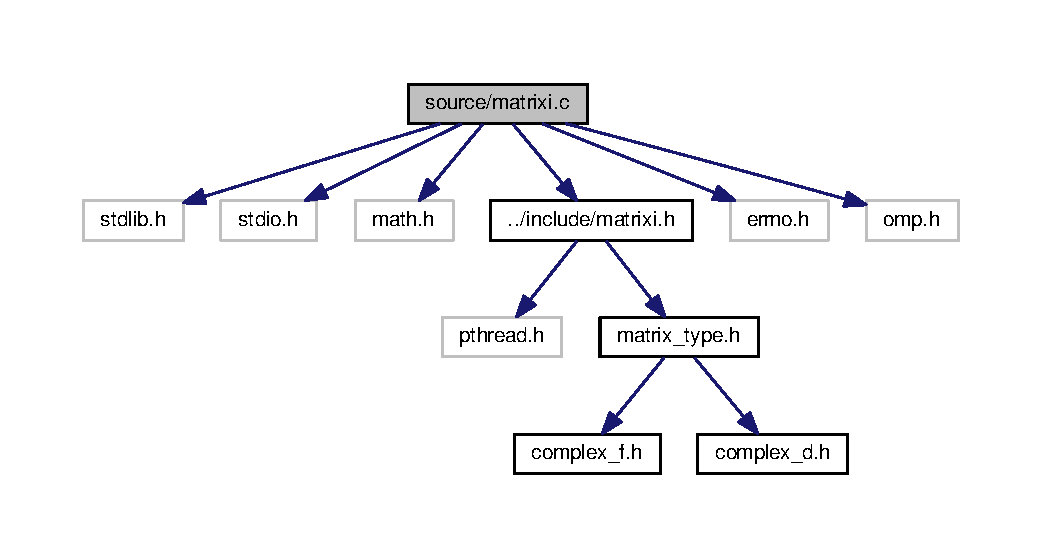
\includegraphics[width=350pt]{matrixi_8c__incl}
\end{center}
\end{figure}
\subsection*{Functions}
\begin{DoxyCompactItemize}
\item 
\hyperlink{structMatrix__i}{Matrix\+\_\+i} $\ast$ \hyperlink{matrixi_8c_a6365f70707f3847b14d55585db05079c}{read\+Matrix\+\_\+i\+\_\+\+File} (char $\ast$filename)
\begin{DoxyCompactList}\small\item\em reads a matrix from a binary file \end{DoxyCompactList}\item 
int \hyperlink{matrixi_8c_a86f0cf175b5a3d31f5678c39c1bf29c5}{write\+Matrix\+\_\+i\+\_\+\+File} (char $\ast$filename, \hyperlink{structMatrix__i}{Matrix\+\_\+i} $\ast$ptr)
\begin{DoxyCompactList}\small\item\em writes a matrix in a binary file \end{DoxyCompactList}\item 
void \hyperlink{matrixi_8c_a3fbc6603dffbe76a797d2cd62fb10ef5}{print\+MatrixI} (\hyperlink{structMatrix__i}{Matrix\+\_\+i} $\ast$a)
\begin{DoxyCompactList}\small\item\em print\+MatrixI display a matrix of ints (usefull for testing) \end{DoxyCompactList}\item 
\hyperlink{structMatrix__i}{Matrix\+\_\+i} $\ast$ \hyperlink{matrixi_8c_a568f89f9c49ca0932c1dc144b93412af}{matrix\+AllocI} (unsigned int rows, unsigned int column)
\begin{DoxyCompactList}\small\item\em matrix\+AllocI allocate memory for a matrix and initialize it to zero \end{DoxyCompactList}\item 
\hyperlink{structMatrix__i}{Matrix\+\_\+i} $\ast$ \hyperlink{matrixi_8c_a231c24a108ef28588fd51d9fc6d695a9}{create\+Random\+MatrixI} (unsigned int rows, unsigned int column)
\begin{DoxyCompactList}\small\item\em create\+Random\+Matrix initialize a random Matrix \end{DoxyCompactList}\item 
void \hyperlink{matrixi_8c_a833ef315c79911810bb846f214076fa2}{create\+Zero\+MatrixI} (\hyperlink{structMatrix__i}{Matrix\+\_\+i} $\ast$J)
\begin{DoxyCompactList}\small\item\em create\+Random\+Matrix initialize a random Matrix \end{DoxyCompactList}\item 
\hyperlink{structMatrix__i}{Matrix\+\_\+i} $\ast$ \hyperlink{matrixi_8c_a8a8eb272471e70bf5ac029f557e47a75}{create\+Test\+VectorI} (unsigned int type)
\begin{DoxyCompactList}\small\item\em create\+Test\+Vector initialize a known vector of size 3\+:1 \end{DoxyCompactList}\item 
void \hyperlink{matrixi_8c_a03cf221e884b960b85ab1d2ba6feef64}{create\+IdentityI} (\hyperlink{structMatrix__i}{Matrix\+\_\+i} $\ast$I)
\begin{DoxyCompactList}\small\item\em create\+IdentityI compute the identoty matrix \end{DoxyCompactList}\item 
void \hyperlink{matrixi_8c_adeb4204ab59b79821519df5387d8a14f}{free\+MatrixI} (\hyperlink{structMatrix__i}{Matrix\+\_\+i} $\ast$A)
\begin{DoxyCompactList}\small\item\em free\+MatrixI free a int matrix \end{DoxyCompactList}\item 
int \hyperlink{matrixi_8c_a1abcdbd4db2d1f6a9b62b54204f1d260}{matrix\+GetI} (\hyperlink{structMatrix__i}{Matrix\+\_\+i} $\ast$A, unsigned int i, unsigned int j)
\begin{DoxyCompactList}\small\item\em matrix\+GetI access a specified data of a matrix \end{DoxyCompactList}\item 
void \hyperlink{matrixi_8c_a43e8ccbdb8c1b5bd7d1a880662fb8f1b}{matrix\+SetI} (\hyperlink{structMatrix__i}{Matrix\+\_\+i} $\ast$A, unsigned int i, unsigned int j, const int c)
\begin{DoxyCompactList}\small\item\em matrix\+SetI set the value of a specified data \end{DoxyCompactList}\item 
void \hyperlink{matrixi_8c_affed5a1f5b929f9100007f6f81b8d803}{scale\+MatrixI} (\hyperlink{structMatrix__i}{Matrix\+\_\+i} $\ast$a, const int c)
\begin{DoxyCompactList}\small\item\em scale\+MatrixI multiply each data by a constant () \end{DoxyCompactList}\item 
void \hyperlink{matrixi_8c_abfab3aa11a314e5e834e8434f74cc71b}{add\+MatrixI} (\hyperlink{structMatrix__i}{Matrix\+\_\+i} $\ast$a, \hyperlink{structMatrix__i}{Matrix\+\_\+i} $\ast$b)
\begin{DoxyCompactList}\small\item\em add\+MatrixI compute A = A+B \end{DoxyCompactList}\item 
void \hyperlink{matrixi_8c_a1b171fa67cd23b75573aec219557daff}{add\+Matrix\+TI} (\hyperlink{structMatrix__i}{Matrix\+\_\+i} $\ast$a, \hyperlink{structMatrix__i}{Matrix\+\_\+i} $\ast$b)
\begin{DoxyCompactList}\small\item\em add\+Matrix\+TI compute A = A+\+BT BT being the transposed matrix of B \end{DoxyCompactList}\item 
void \hyperlink{matrixi_8c_afdd474d6f463ca59cc602c0cfdaa2abc}{sub\+MatrixI} (\hyperlink{structMatrix__i}{Matrix\+\_\+i} $\ast$a, \hyperlink{structMatrix__i}{Matrix\+\_\+i} $\ast$b)
\begin{DoxyCompactList}\small\item\em sub\+MatrixI compute A = A-\/B \end{DoxyCompactList}\item 
void \hyperlink{matrixi_8c_a7d426eaee61f753f65c7322b9880c9e4}{mul\+MatrixI} (\hyperlink{structMatrix__i}{Matrix\+\_\+i} $\ast$a, \hyperlink{structMatrix__i}{Matrix\+\_\+i} $\ast$b, \hyperlink{structMatrix__i}{Matrix\+\_\+i} $\ast$c)
\begin{DoxyCompactList}\small\item\em compute C = A$\ast$B \end{DoxyCompactList}\item 
void \hyperlink{matrixi_8c_a76384782aae46dc752fd395fb06c9218}{mat\+RefI} (\hyperlink{structMatrix__i}{Matrix\+\_\+i} $\ast$A)
\begin{DoxyCompactList}\small\item\em mat\+NormI take the first matrix A value as a reference (ie\+: 1) and scale the other value accoarding to that \end{DoxyCompactList}\item 
void \hyperlink{matrixi_8c_ab2e82c1f99fc800dc3e1e99cf24461cc}{scale\+LineI} (\hyperlink{structMatrix__i}{Matrix\+\_\+i} $\ast$a, unsigned int i, int f)
\begin{DoxyCompactList}\small\item\em scale\+LineI multiply a line with a \end{DoxyCompactList}\item 
int \hyperlink{matrixi_8c_a3d13c42bad8b98628d4b640c47b8ea1e}{sub\+X\+LinesI} (\hyperlink{structMatrix__i}{Matrix\+\_\+i} $\ast$a, unsigned int i, unsigned int i2, int f)
\begin{DoxyCompactList}\small\item\em sub\+X\+LinesI computes line i -\/ f$\ast$line i2 and store it into line i \end{DoxyCompactList}\item 
void \hyperlink{matrixi_8c_a5e938926ea3b0d47f616d5c38dc40a6c}{mul\+Add\+Scale\+MatrixI} (\hyperlink{structMatrix__i}{Matrix\+\_\+i} $\ast$result, \hyperlink{structMatrix__i}{Matrix\+\_\+i} $\ast$mul1, \hyperlink{structMatrix__i}{Matrix\+\_\+i} $\ast$mul2, \hyperlink{structMatrix__i}{Matrix\+\_\+i} $\ast$add, int l, int s)
\begin{DoxyCompactList}\small\item\em compute result = s$\ast$(mul1$\ast$mul2 + l$\ast$add) \end{DoxyCompactList}\item 
int \hyperlink{matrixi_8c_a3786a01891f5bf203a730e99140c848b}{is\+DiagI} (\hyperlink{structMatrix__i}{Matrix\+\_\+i} $\ast$a)
\begin{DoxyCompactList}\small\item\em checks if the matrix is diagonal and sets its flag if necessary \end{DoxyCompactList}\item 
int \hyperlink{matrixi_8c_ae0b435187baf326bdf4d262bc6157d31}{is\+Tri\+UI} (\hyperlink{structMatrix__i}{Matrix\+\_\+i} $\ast$a)
\begin{DoxyCompactList}\small\item\em checks if the matrix is triangular UP and sets its flag if necessary \end{DoxyCompactList}\item 
int \hyperlink{matrixi_8c_ac27fd76e1d91d7029e863dfe78d8e18a}{is\+Tri\+LI} (\hyperlink{structMatrix__i}{Matrix\+\_\+i} $\ast$a)
\begin{DoxyCompactList}\small\item\em checks if the matrix is triangular Low and sets its flag if necessary \end{DoxyCompactList}\item 
int \hyperlink{matrixi_8c_a0b6dcca2d7552e4f6d8dfb6b7b73d24d}{is\+SparseI} (\hyperlink{structMatrix__i}{Matrix\+\_\+i} $\ast$a)
\begin{DoxyCompactList}\small\item\em checks if the sparcity of the matrix is superior to 2/3 (allows compression) \end{DoxyCompactList}\end{DoxyCompactItemize}


\subsection{Detailed Description}
to handle matrix operations for integers \begin{DoxyAuthor}{Author}
Nicolas Sourbier 
\end{DoxyAuthor}
\begin{DoxyDate}{Date}
10/09/2018 
\end{DoxyDate}


\subsection{Function Documentation}
\index{matrixi.\+c@{matrixi.\+c}!add\+MatrixI@{add\+MatrixI}}
\index{add\+MatrixI@{add\+MatrixI}!matrixi.\+c@{matrixi.\+c}}
\subsubsection[{\texorpdfstring{add\+Matrix\+I(\+Matrix\+\_\+i $\ast$a, Matrix\+\_\+i $\ast$b)}{addMatrixI(Matrix_i *a, Matrix_i *b)}}]{\setlength{\rightskip}{0pt plus 5cm}void add\+MatrixI (
\begin{DoxyParamCaption}
\item[{{\bf Matrix\+\_\+i} $\ast$}]{a, }
\item[{{\bf Matrix\+\_\+i} $\ast$}]{b}
\end{DoxyParamCaption}
)}\hypertarget{matrixi_8c_abfab3aa11a314e5e834e8434f74cc71b}{}\label{matrixi_8c_abfab3aa11a314e5e834e8434f74cc71b}


add\+MatrixI compute A = A+B 


\begin{DoxyParams}{Parameters}
{\em a} & matrix \\
\hline
{\em b} & matrix \\
\hline
\end{DoxyParams}
\begin{DoxyRefDesc}{Todo}
\item[\hyperlink{todo__todo000002}{Todo}]Parallel programming \end{DoxyRefDesc}
\index{matrixi.\+c@{matrixi.\+c}!add\+Matrix\+TI@{add\+Matrix\+TI}}
\index{add\+Matrix\+TI@{add\+Matrix\+TI}!matrixi.\+c@{matrixi.\+c}}
\subsubsection[{\texorpdfstring{add\+Matrix\+T\+I(\+Matrix\+\_\+i $\ast$a, Matrix\+\_\+i $\ast$b)}{addMatrixTI(Matrix_i *a, Matrix_i *b)}}]{\setlength{\rightskip}{0pt plus 5cm}void add\+Matrix\+TI (
\begin{DoxyParamCaption}
\item[{{\bf Matrix\+\_\+i} $\ast$}]{a, }
\item[{{\bf Matrix\+\_\+i} $\ast$}]{b}
\end{DoxyParamCaption}
)}\hypertarget{matrixi_8c_a1b171fa67cd23b75573aec219557daff}{}\label{matrixi_8c_a1b171fa67cd23b75573aec219557daff}


add\+Matrix\+TI compute A = A+\+BT BT being the transposed matrix of B 


\begin{DoxyParams}{Parameters}
{\em a} & matrix \\
\hline
{\em b} & matrix \\
\hline
\end{DoxyParams}
\begin{DoxyRefDesc}{Todo}
\item[\hyperlink{todo__todo000003}{Todo}]Parallel programming \end{DoxyRefDesc}
\index{matrixi.\+c@{matrixi.\+c}!create\+IdentityI@{create\+IdentityI}}
\index{create\+IdentityI@{create\+IdentityI}!matrixi.\+c@{matrixi.\+c}}
\subsubsection[{\texorpdfstring{create\+Identity\+I(\+Matrix\+\_\+i $\ast$\+I)}{createIdentityI(Matrix_i *I)}}]{\setlength{\rightskip}{0pt plus 5cm}void create\+IdentityI (
\begin{DoxyParamCaption}
\item[{{\bf Matrix\+\_\+i} $\ast$}]{}
\end{DoxyParamCaption}
)}\hypertarget{matrixi_8c_a03cf221e884b960b85ab1d2ba6feef64}{}\label{matrixi_8c_a03cf221e884b960b85ab1d2ba6feef64}


create\+IdentityI compute the identoty matrix 


\begin{DoxyParams}{Parameters}
{\em I} & A pointer to store the result \\
\hline
\end{DoxyParams}
\index{matrixi.\+c@{matrixi.\+c}!create\+Random\+MatrixI@{create\+Random\+MatrixI}}
\index{create\+Random\+MatrixI@{create\+Random\+MatrixI}!matrixi.\+c@{matrixi.\+c}}
\subsubsection[{\texorpdfstring{create\+Random\+Matrix\+I(unsigned int rows, unsigned int column)}{createRandomMatrixI(unsigned int rows, unsigned int column)}}]{\setlength{\rightskip}{0pt plus 5cm}{\bf Matrix\+\_\+i}$\ast$ create\+Random\+MatrixI (
\begin{DoxyParamCaption}
\item[{unsigned int}]{rows, }
\item[{unsigned int}]{column}
\end{DoxyParamCaption}
)}\hypertarget{matrixi_8c_a231c24a108ef28588fd51d9fc6d695a9}{}\label{matrixi_8c_a231c24a108ef28588fd51d9fc6d695a9}


create\+Random\+Matrix initialize a random Matrix 


\begin{DoxyParams}{Parameters}
{\em rows} & number of rows \\
\hline
{\em column} & number of columns \\
\hline
\end{DoxyParams}
\begin{DoxyReturn}{Returns}
the random matrix 
\end{DoxyReturn}
\index{matrixi.\+c@{matrixi.\+c}!create\+Test\+VectorI@{create\+Test\+VectorI}}
\index{create\+Test\+VectorI@{create\+Test\+VectorI}!matrixi.\+c@{matrixi.\+c}}
\subsubsection[{\texorpdfstring{create\+Test\+Vector\+I(unsigned int type)}{createTestVectorI(unsigned int type)}}]{\setlength{\rightskip}{0pt plus 5cm}{\bf Matrix\+\_\+i}$\ast$ create\+Test\+VectorI (
\begin{DoxyParamCaption}
\item[{unsigned int}]{type}
\end{DoxyParamCaption}
)}\hypertarget{matrixi_8c_a8a8eb272471e70bf5ac029f557e47a75}{}\label{matrixi_8c_a8a8eb272471e70bf5ac029f557e47a75}


create\+Test\+Vector initialize a known vector of size 3\+:1 


\begin{DoxyParams}{Parameters}
{\em rows} & number of rows \\
\hline
{\em column} & number of columns \\
\hline
\end{DoxyParams}
\begin{DoxyReturn}{Returns}
the random matrix 
\end{DoxyReturn}
\index{matrixi.\+c@{matrixi.\+c}!create\+Zero\+MatrixI@{create\+Zero\+MatrixI}}
\index{create\+Zero\+MatrixI@{create\+Zero\+MatrixI}!matrixi.\+c@{matrixi.\+c}}
\subsubsection[{\texorpdfstring{create\+Zero\+Matrix\+I(\+Matrix\+\_\+i $\ast$\+J)}{createZeroMatrixI(Matrix_i *J)}}]{\setlength{\rightskip}{0pt plus 5cm}void create\+Zero\+MatrixI (
\begin{DoxyParamCaption}
\item[{{\bf Matrix\+\_\+i} $\ast$}]{J}
\end{DoxyParamCaption}
)}\hypertarget{matrixi_8c_a833ef315c79911810bb846f214076fa2}{}\label{matrixi_8c_a833ef315c79911810bb846f214076fa2}


create\+Random\+Matrix initialize a random Matrix 


\begin{DoxyParams}{Parameters}
{\em rows} & number of rows \\
\hline
{\em column} & number of columns \\
\hline
\end{DoxyParams}
\begin{DoxyReturn}{Returns}
the random matrix 
\end{DoxyReturn}
\index{matrixi.\+c@{matrixi.\+c}!free\+MatrixI@{free\+MatrixI}}
\index{free\+MatrixI@{free\+MatrixI}!matrixi.\+c@{matrixi.\+c}}
\subsubsection[{\texorpdfstring{free\+Matrix\+I(\+Matrix\+\_\+i $\ast$\+A)}{freeMatrixI(Matrix_i *A)}}]{\setlength{\rightskip}{0pt plus 5cm}void free\+MatrixI (
\begin{DoxyParamCaption}
\item[{{\bf Matrix\+\_\+i} $\ast$}]{A}
\end{DoxyParamCaption}
)}\hypertarget{matrixi_8c_adeb4204ab59b79821519df5387d8a14f}{}\label{matrixi_8c_adeb4204ab59b79821519df5387d8a14f}


free\+MatrixI free a int matrix 


\begin{DoxyParams}{Parameters}
{\em A} & the matrix to free \\
\hline
\end{DoxyParams}
\index{matrixi.\+c@{matrixi.\+c}!is\+DiagI@{is\+DiagI}}
\index{is\+DiagI@{is\+DiagI}!matrixi.\+c@{matrixi.\+c}}
\subsubsection[{\texorpdfstring{is\+Diag\+I(\+Matrix\+\_\+i $\ast$a)}{isDiagI(Matrix_i *a)}}]{\setlength{\rightskip}{0pt plus 5cm}int is\+DiagI (
\begin{DoxyParamCaption}
\item[{{\bf Matrix\+\_\+i} $\ast$}]{a}
\end{DoxyParamCaption}
)}\hypertarget{matrixi_8c_a3786a01891f5bf203a730e99140c848b}{}\label{matrixi_8c_a3786a01891f5bf203a730e99140c848b}


checks if the matrix is diagonal and sets its flag if necessary 


\begin{DoxyParams}{Parameters}
{\em a} & the matrix to test returns 1 if diag, 0 otherwise \\
\hline
\end{DoxyParams}
\index{matrixi.\+c@{matrixi.\+c}!is\+SparseI@{is\+SparseI}}
\index{is\+SparseI@{is\+SparseI}!matrixi.\+c@{matrixi.\+c}}
\subsubsection[{\texorpdfstring{is\+Sparse\+I(\+Matrix\+\_\+i $\ast$a)}{isSparseI(Matrix_i *a)}}]{\setlength{\rightskip}{0pt plus 5cm}int is\+SparseI (
\begin{DoxyParamCaption}
\item[{{\bf Matrix\+\_\+i} $\ast$}]{a}
\end{DoxyParamCaption}
)}\hypertarget{matrixi_8c_a0b6dcca2d7552e4f6d8dfb6b7b73d24d}{}\label{matrixi_8c_a0b6dcca2d7552e4f6d8dfb6b7b73d24d}


checks if the sparcity of the matrix is superior to 2/3 (allows compression) 


\begin{DoxyParams}{Parameters}
{\em a} & the matrix to test returns 1 if diag, 0 otherwise \\
\hline
\end{DoxyParams}
\index{matrixi.\+c@{matrixi.\+c}!is\+Tri\+LI@{is\+Tri\+LI}}
\index{is\+Tri\+LI@{is\+Tri\+LI}!matrixi.\+c@{matrixi.\+c}}
\subsubsection[{\texorpdfstring{is\+Tri\+L\+I(\+Matrix\+\_\+i $\ast$a)}{isTriLI(Matrix_i *a)}}]{\setlength{\rightskip}{0pt plus 5cm}int is\+Tri\+LI (
\begin{DoxyParamCaption}
\item[{{\bf Matrix\+\_\+i} $\ast$}]{a}
\end{DoxyParamCaption}
)}\hypertarget{matrixi_8c_ac27fd76e1d91d7029e863dfe78d8e18a}{}\label{matrixi_8c_ac27fd76e1d91d7029e863dfe78d8e18a}


checks if the matrix is triangular Low and sets its flag if necessary 


\begin{DoxyParams}{Parameters}
{\em a} & the matrix to test returns 1 if diag, 0 otherwise \\
\hline
\end{DoxyParams}
\index{matrixi.\+c@{matrixi.\+c}!is\+Tri\+UI@{is\+Tri\+UI}}
\index{is\+Tri\+UI@{is\+Tri\+UI}!matrixi.\+c@{matrixi.\+c}}
\subsubsection[{\texorpdfstring{is\+Tri\+U\+I(\+Matrix\+\_\+i $\ast$a)}{isTriUI(Matrix_i *a)}}]{\setlength{\rightskip}{0pt plus 5cm}int is\+Tri\+UI (
\begin{DoxyParamCaption}
\item[{{\bf Matrix\+\_\+i} $\ast$}]{a}
\end{DoxyParamCaption}
)}\hypertarget{matrixi_8c_ae0b435187baf326bdf4d262bc6157d31}{}\label{matrixi_8c_ae0b435187baf326bdf4d262bc6157d31}


checks if the matrix is triangular UP and sets its flag if necessary 


\begin{DoxyParams}{Parameters}
{\em a} & the matrix to test returns 1 if diag, 0 otherwise \\
\hline
\end{DoxyParams}
\index{matrixi.\+c@{matrixi.\+c}!mat\+RefI@{mat\+RefI}}
\index{mat\+RefI@{mat\+RefI}!matrixi.\+c@{matrixi.\+c}}
\subsubsection[{\texorpdfstring{mat\+Ref\+I(\+Matrix\+\_\+i $\ast$\+A)}{matRefI(Matrix_i *A)}}]{\setlength{\rightskip}{0pt plus 5cm}void mat\+RefI (
\begin{DoxyParamCaption}
\item[{{\bf Matrix\+\_\+i} $\ast$}]{A}
\end{DoxyParamCaption}
)}\hypertarget{matrixi_8c_a76384782aae46dc752fd395fb06c9218}{}\label{matrixi_8c_a76384782aae46dc752fd395fb06c9218}


mat\+NormI take the first matrix A value as a reference (ie\+: 1) and scale the other value accoarding to that 


\begin{DoxyParams}{Parameters}
{\em A} & the matrix that we want to \char`\"{}norm\char`\"{} \\
\hline
\end{DoxyParams}
\index{matrixi.\+c@{matrixi.\+c}!matrix\+AllocI@{matrix\+AllocI}}
\index{matrix\+AllocI@{matrix\+AllocI}!matrixi.\+c@{matrixi.\+c}}
\subsubsection[{\texorpdfstring{matrix\+Alloc\+I(unsigned int rows, unsigned int column)}{matrixAllocI(unsigned int rows, unsigned int column)}}]{\setlength{\rightskip}{0pt plus 5cm}{\bf Matrix\+\_\+i}$\ast$ matrix\+AllocI (
\begin{DoxyParamCaption}
\item[{unsigned int}]{rows, }
\item[{unsigned int}]{column}
\end{DoxyParamCaption}
)}\hypertarget{matrixi_8c_a568f89f9c49ca0932c1dc144b93412af}{}\label{matrixi_8c_a568f89f9c49ca0932c1dc144b93412af}


matrix\+AllocI allocate memory for a matrix and initialize it to zero 


\begin{DoxyParams}{Parameters}
{\em rows} & number of rows \\
\hline
{\em column} & number of columns \\
\hline
\end{DoxyParams}
\begin{DoxyReturn}{Returns}
the allocated matrix if no errors occured, N\+U\+LL if not 
\end{DoxyReturn}
\index{matrixi.\+c@{matrixi.\+c}!matrix\+GetI@{matrix\+GetI}}
\index{matrix\+GetI@{matrix\+GetI}!matrixi.\+c@{matrixi.\+c}}
\subsubsection[{\texorpdfstring{matrix\+Get\+I(\+Matrix\+\_\+i $\ast$\+A, unsigned int i, unsigned int j)}{matrixGetI(Matrix_i *A, unsigned int i, unsigned int j)}}]{\setlength{\rightskip}{0pt plus 5cm}int matrix\+GetI (
\begin{DoxyParamCaption}
\item[{{\bf Matrix\+\_\+i} $\ast$}]{A, }
\item[{unsigned int}]{i, }
\item[{unsigned int}]{j}
\end{DoxyParamCaption}
)}\hypertarget{matrixi_8c_a1abcdbd4db2d1f6a9b62b54204f1d260}{}\label{matrixi_8c_a1abcdbd4db2d1f6a9b62b54204f1d260}


matrix\+GetI access a specified data of a matrix 


\begin{DoxyParams}{Parameters}
{\em A} & the matrix \\
\hline
{\em i} & the index of rows \\
\hline
{\em j} & the index on columns \\
\hline
\end{DoxyParams}
\begin{DoxyReturn}{Returns}
the data A(i,j) 
\end{DoxyReturn}
\begin{DoxyWarning}{Warning}
if the matrix in parameter is N\+U\+LL, returns 0 
\end{DoxyWarning}
\index{matrixi.\+c@{matrixi.\+c}!matrix\+SetI@{matrix\+SetI}}
\index{matrix\+SetI@{matrix\+SetI}!matrixi.\+c@{matrixi.\+c}}
\subsubsection[{\texorpdfstring{matrix\+Set\+I(\+Matrix\+\_\+i $\ast$\+A, unsigned int i, unsigned int j, const int c)}{matrixSetI(Matrix_i *A, unsigned int i, unsigned int j, const int c)}}]{\setlength{\rightskip}{0pt plus 5cm}void matrix\+SetI (
\begin{DoxyParamCaption}
\item[{{\bf Matrix\+\_\+i} $\ast$}]{A, }
\item[{unsigned int}]{i, }
\item[{unsigned int}]{j, }
\item[{const int}]{c}
\end{DoxyParamCaption}
)}\hypertarget{matrixi_8c_a43e8ccbdb8c1b5bd7d1a880662fb8f1b}{}\label{matrixi_8c_a43e8ccbdb8c1b5bd7d1a880662fb8f1b}


matrix\+SetI set the value of a specified data 


\begin{DoxyParams}{Parameters}
{\em A} & the matrix \\
\hline
{\em i} & the index on rows \\
\hline
{\em j} & the index on columns \\
\hline
{\em c} & the to set at A(i,j) \\
\hline
\end{DoxyParams}
\index{matrixi.\+c@{matrixi.\+c}!mul\+Add\+Scale\+MatrixI@{mul\+Add\+Scale\+MatrixI}}
\index{mul\+Add\+Scale\+MatrixI@{mul\+Add\+Scale\+MatrixI}!matrixi.\+c@{matrixi.\+c}}
\subsubsection[{\texorpdfstring{mul\+Add\+Scale\+Matrix\+I(\+Matrix\+\_\+i $\ast$result, Matrix\+\_\+i $\ast$mul1, Matrix\+\_\+i $\ast$mul2, Matrix\+\_\+i $\ast$add, int l, int s)}{mulAddScaleMatrixI(Matrix_i *result, Matrix_i *mul1, Matrix_i *mul2, Matrix_i *add, int l, int s)}}]{\setlength{\rightskip}{0pt plus 5cm}void mul\+Add\+Scale\+MatrixI (
\begin{DoxyParamCaption}
\item[{{\bf Matrix\+\_\+i} $\ast$}]{result, }
\item[{{\bf Matrix\+\_\+i} $\ast$}]{mul1, }
\item[{{\bf Matrix\+\_\+i} $\ast$}]{mul2, }
\item[{{\bf Matrix\+\_\+i} $\ast$}]{add, }
\item[{int}]{l, }
\item[{int}]{s}
\end{DoxyParamCaption}
)}\hypertarget{matrixi_8c_a5e938926ea3b0d47f616d5c38dc40a6c}{}\label{matrixi_8c_a5e938926ea3b0d47f616d5c38dc40a6c}


compute result = s$\ast$(mul1$\ast$mul2 + l$\ast$add) 


\begin{DoxyParams}{Parameters}
{\em result} & a matrix to store the result \\
\hline
{\em mul1} & \& mul2 matrices to multiply \\
\hline
{\em add} & a matrix to add to the previous product \\
\hline
{\em l} & a int to scale the add matrix \\
\hline
{\em s} & a int to scale the result doesn\textquotesingle{}t use optimisations related to the matrix properties \\
\hline
\end{DoxyParams}
\index{matrixi.\+c@{matrixi.\+c}!mul\+MatrixI@{mul\+MatrixI}}
\index{mul\+MatrixI@{mul\+MatrixI}!matrixi.\+c@{matrixi.\+c}}
\subsubsection[{\texorpdfstring{mul\+Matrix\+I(\+Matrix\+\_\+i $\ast$a, Matrix\+\_\+i $\ast$b, Matrix\+\_\+i $\ast$c)}{mulMatrixI(Matrix_i *a, Matrix_i *b, Matrix_i *c)}}]{\setlength{\rightskip}{0pt plus 5cm}void mul\+MatrixI (
\begin{DoxyParamCaption}
\item[{{\bf Matrix\+\_\+i} $\ast$}]{a, }
\item[{{\bf Matrix\+\_\+i} $\ast$}]{b, }
\item[{{\bf Matrix\+\_\+i} $\ast$}]{c}
\end{DoxyParamCaption}
)}\hypertarget{matrixi_8c_a7d426eaee61f753f65c7322b9880c9e4}{}\label{matrixi_8c_a7d426eaee61f753f65c7322b9880c9e4}


compute C = A$\ast$B 


\begin{DoxyParams}{Parameters}
{\em a} & matrix \\
\hline
{\em b} & matrix \\
\hline
{\em c} & a matrix to store the result \\
\hline
\end{DoxyParams}
\index{matrixi.\+c@{matrixi.\+c}!print\+MatrixI@{print\+MatrixI}}
\index{print\+MatrixI@{print\+MatrixI}!matrixi.\+c@{matrixi.\+c}}
\subsubsection[{\texorpdfstring{print\+Matrix\+I(\+Matrix\+\_\+i $\ast$a)}{printMatrixI(Matrix_i *a)}}]{\setlength{\rightskip}{0pt plus 5cm}void print\+MatrixI (
\begin{DoxyParamCaption}
\item[{{\bf Matrix\+\_\+i} $\ast$}]{a}
\end{DoxyParamCaption}
)}\hypertarget{matrixi_8c_a3fbc6603dffbe76a797d2cd62fb10ef5}{}\label{matrixi_8c_a3fbc6603dffbe76a797d2cd62fb10ef5}


print\+MatrixI display a matrix of ints (usefull for testing) 


\begin{DoxyParams}{Parameters}
{\em a} & the matrix to display \\
\hline
\end{DoxyParams}
\index{matrixi.\+c@{matrixi.\+c}!read\+Matrix\+\_\+i\+\_\+\+File@{read\+Matrix\+\_\+i\+\_\+\+File}}
\index{read\+Matrix\+\_\+i\+\_\+\+File@{read\+Matrix\+\_\+i\+\_\+\+File}!matrixi.\+c@{matrixi.\+c}}
\subsubsection[{\texorpdfstring{read\+Matrix\+\_\+i\+\_\+\+File(char $\ast$filename)}{readMatrix_i_File(char *filename)}}]{\setlength{\rightskip}{0pt plus 5cm}{\bf Matrix\+\_\+i}$\ast$ read\+Matrix\+\_\+i\+\_\+\+File (
\begin{DoxyParamCaption}
\item[{char $\ast$}]{filename}
\end{DoxyParamCaption}
)}\hypertarget{matrixi_8c_a6365f70707f3847b14d55585db05079c}{}\label{matrixi_8c_a6365f70707f3847b14d55585db05079c}


reads a matrix from a binary file 


\begin{DoxyParams}{Parameters}
{\em filename} & the name of the file where the matrix is writen \\
\hline
\end{DoxyParams}
\begin{DoxyReturn}{Returns}
the writen matrix N\+U\+LL if there was an error 
\end{DoxyReturn}
\index{matrixi.\+c@{matrixi.\+c}!scale\+LineI@{scale\+LineI}}
\index{scale\+LineI@{scale\+LineI}!matrixi.\+c@{matrixi.\+c}}
\subsubsection[{\texorpdfstring{scale\+Line\+I(\+Matrix\+\_\+i $\ast$a, unsigned int i, int f)}{scaleLineI(Matrix_i *a, unsigned int i, int f)}}]{\setlength{\rightskip}{0pt plus 5cm}void scale\+LineI (
\begin{DoxyParamCaption}
\item[{{\bf Matrix\+\_\+i} $\ast$}]{a, }
\item[{unsigned int}]{i, }
\item[{int}]{f}
\end{DoxyParamCaption}
)}\hypertarget{matrixi_8c_ab2e82c1f99fc800dc3e1e99cf24461cc}{}\label{matrixi_8c_ab2e82c1f99fc800dc3e1e99cf24461cc}


scale\+LineI multiply a line with a 


\begin{DoxyParams}{Parameters}
{\em a} & the matrix \\
\hline
{\em i} & the index of the line we want to scale \\
\hline
{\em f} & the that will scale the line \\
\hline
\end{DoxyParams}
\index{matrixi.\+c@{matrixi.\+c}!scale\+MatrixI@{scale\+MatrixI}}
\index{scale\+MatrixI@{scale\+MatrixI}!matrixi.\+c@{matrixi.\+c}}
\subsubsection[{\texorpdfstring{scale\+Matrix\+I(\+Matrix\+\_\+i $\ast$a, const int c)}{scaleMatrixI(Matrix_i *a, const int c)}}]{\setlength{\rightskip}{0pt plus 5cm}void scale\+MatrixI (
\begin{DoxyParamCaption}
\item[{{\bf Matrix\+\_\+i} $\ast$}]{a, }
\item[{const int}]{c}
\end{DoxyParamCaption}
)}\hypertarget{matrixi_8c_affed5a1f5b929f9100007f6f81b8d803}{}\label{matrixi_8c_affed5a1f5b929f9100007f6f81b8d803}


scale\+MatrixI multiply each data by a constant () 


\begin{DoxyParams}{Parameters}
{\em a} & the matrix to scale \\
\hline
{\em c} & the \\
\hline
\end{DoxyParams}
\begin{DoxyRefDesc}{Todo}
\item[\hyperlink{todo__todo000001}{Todo}]Parallel programming \end{DoxyRefDesc}
\index{matrixi.\+c@{matrixi.\+c}!sub\+MatrixI@{sub\+MatrixI}}
\index{sub\+MatrixI@{sub\+MatrixI}!matrixi.\+c@{matrixi.\+c}}
\subsubsection[{\texorpdfstring{sub\+Matrix\+I(\+Matrix\+\_\+i $\ast$a, Matrix\+\_\+i $\ast$b)}{subMatrixI(Matrix_i *a, Matrix_i *b)}}]{\setlength{\rightskip}{0pt plus 5cm}void sub\+MatrixI (
\begin{DoxyParamCaption}
\item[{{\bf Matrix\+\_\+i} $\ast$}]{a, }
\item[{{\bf Matrix\+\_\+i} $\ast$}]{b}
\end{DoxyParamCaption}
)}\hypertarget{matrixi_8c_afdd474d6f463ca59cc602c0cfdaa2abc}{}\label{matrixi_8c_afdd474d6f463ca59cc602c0cfdaa2abc}


sub\+MatrixI compute A = A-\/B 


\begin{DoxyParams}{Parameters}
{\em a} & matrix \\
\hline
{\em b} & matrix \\
\hline
\end{DoxyParams}
\begin{DoxyRefDesc}{Todo}
\item[\hyperlink{todo__todo000004}{Todo}]Parallel programming \end{DoxyRefDesc}
\index{matrixi.\+c@{matrixi.\+c}!sub\+X\+LinesI@{sub\+X\+LinesI}}
\index{sub\+X\+LinesI@{sub\+X\+LinesI}!matrixi.\+c@{matrixi.\+c}}
\subsubsection[{\texorpdfstring{sub\+X\+Lines\+I(\+Matrix\+\_\+i $\ast$a, unsigned int i, unsigned int i2, int f)}{subXLinesI(Matrix_i *a, unsigned int i, unsigned int i2, int f)}}]{\setlength{\rightskip}{0pt plus 5cm}int sub\+X\+LinesI (
\begin{DoxyParamCaption}
\item[{{\bf Matrix\+\_\+i} $\ast$}]{a, }
\item[{unsigned int}]{i, }
\item[{unsigned int}]{i2, }
\item[{int}]{f}
\end{DoxyParamCaption}
)}\hypertarget{matrixi_8c_a3d13c42bad8b98628d4b640c47b8ea1e}{}\label{matrixi_8c_a3d13c42bad8b98628d4b640c47b8ea1e}


sub\+X\+LinesI computes line i -\/ f$\ast$line i2 and store it into line i 


\begin{DoxyParams}{Parameters}
{\em a} & the matrix \\
\hline
{\em i} & the index of the line to update \\
\hline
{\em i2} & the index of the \char`\"{}reference\char`\"{} line \\
\hline
{\em f} & a to scale the matrix \\
\hline
\end{DoxyParams}
\index{matrixi.\+c@{matrixi.\+c}!write\+Matrix\+\_\+i\+\_\+\+File@{write\+Matrix\+\_\+i\+\_\+\+File}}
\index{write\+Matrix\+\_\+i\+\_\+\+File@{write\+Matrix\+\_\+i\+\_\+\+File}!matrixi.\+c@{matrixi.\+c}}
\subsubsection[{\texorpdfstring{write\+Matrix\+\_\+i\+\_\+\+File(char $\ast$filename, Matrix\+\_\+i $\ast$ptr)}{writeMatrix_i_File(char *filename, Matrix_i *ptr)}}]{\setlength{\rightskip}{0pt plus 5cm}int write\+Matrix\+\_\+i\+\_\+\+File (
\begin{DoxyParamCaption}
\item[{char $\ast$}]{filename, }
\item[{{\bf Matrix\+\_\+i} $\ast$}]{ptr}
\end{DoxyParamCaption}
)}\hypertarget{matrixi_8c_a86f0cf175b5a3d31f5678c39c1bf29c5}{}\label{matrixi_8c_a86f0cf175b5a3d31f5678c39c1bf29c5}


writes a matrix in a binary file 


\begin{DoxyParams}{Parameters}
{\em filename} & the name of the file where the matrix is writen \\
\hline
{\em ptr} & the matrix to write \\
\hline
\end{DoxyParams}
\begin{DoxyReturn}{Returns}
1 on success 0 otherwise 
\end{DoxyReturn}

%--- End generated contents ---

% Index
\backmatter
\newpage
\phantomsection
\clearemptydoublepage
\addcontentsline{toc}{chapter}{Index}
\printindex

\end{document}
